\documentclass[a4paper]{book}
\usepackage{makeidx}
\usepackage{graphicx}
\usepackage{multicol}
\usepackage{float}
\usepackage{listings}
\usepackage{color}
\usepackage{ifthen}
\usepackage[table]{xcolor}
\usepackage{textcomp}
\usepackage{alltt}
\usepackage{ifpdf}
\ifpdf
\usepackage[pdftex,
            pagebackref=true,
            colorlinks=true,
            linkcolor=blue,
            unicode
           ]{hyperref}
\else
\usepackage[ps2pdf,
            pagebackref=true,
            colorlinks=true,
            linkcolor=blue,
            unicode
           ]{hyperref}
\usepackage{pspicture}
\fi
\usepackage[utf8]{inputenc}
\usepackage{mathptmx}
\usepackage[scaled=.90]{helvet}
\usepackage{courier}
\usepackage{doxygen}
\lstset{language=C++,inputencoding=utf8,basicstyle=\footnotesize,breaklines=true,breakatwhitespace=true,tabsize=4,numbers=left }
\makeindex
\setcounter{tocdepth}{3}
\renewcommand{\footrulewidth}{0.4pt}
\begin{document}
\hypersetup{pageanchor=false}
\begin{titlepage}
\vspace*{7cm}
\begin{center}
{\Large Universal Scheduler \\[1ex]\large 0.0.0 }\\
\vspace*{1cm}
{\large Generated by Doxygen 1.7.3}\\
\vspace*{0.5cm}
{\small Mon Mar 5 2012 17:31:39}\\
\end{center}
\end{titlepage}
\clearemptydoublepage
\pagenumbering{roman}
\tableofcontents
\clearemptydoublepage
\pagenumbering{arabic}
\hypersetup{pageanchor=true}
\chapter{Namespace Index}
\section{Namespace List}
Here is a list of all namespaces with brief descriptions:\begin{DoxyCompactList}
\item\contentsline{section}{\hyperlink{namespaceCore}{Core} }{\pageref{d3/d7a/namespaceCore}}{}
\item\contentsline{section}{\hyperlink{namespacecore}{core} (\hyperlink{namespaceCore}{Core} model classes )}{\pageref{d9/d0f/namespacecore}}{}
\item\contentsline{section}{\hyperlink{namespacestorage}{storage} }{\pageref{d0/daa/namespacestorage}}{}
\item\contentsline{section}{\hyperlink{namespaceStorage}{Storage} }{\pageref{de/d4e/namespaceStorage}}{}
\item\contentsline{section}{\hyperlink{namespaceUI}{UI} }{\pageref{d6/d56/namespaceUI}}{}
\item\contentsline{section}{\hyperlink{namespaceuiconsole}{uiconsole} }{\pageref{da/de1/namespaceuiconsole}}{}
\end{DoxyCompactList}

\chapter{Class Index}
\section{Class Hierarchy}
This inheritance list is sorted roughly, but not completely, alphabetically:\begin{DoxyCompactList}
\item \contentsline{section}{Calendar}{\pageref{dd/dac/classCalendar}}{}
\item \contentsline{section}{storage::CalendarBunch\_\-}{\pageref{d9/de4/structstorage_1_1CalendarBunch__}}{}
\item \contentsline{section}{uiconsole::Command}{\pageref{dc/df0/classuiconsole_1_1Command}}{}
\begin{DoxyCompactList}
\item \contentsline{section}{uiconsole::Command\_\-Add}{\pageref{dd/d31/classuiconsole_1_1Command__Add}}{}
\item \contentsline{section}{uiconsole::Command\_\-All}{\pageref{de/dfe/classuiconsole_1_1Command__All}}{}
\item \contentsline{section}{uiconsole::Command\_\-Clone}{\pageref{df/d75/classuiconsole_1_1Command__Clone}}{}
\item \contentsline{section}{uiconsole::Command\_\-Exclude}{\pageref{d8/d1d/classuiconsole_1_1Command__Exclude}}{}
\item \contentsline{section}{uiconsole::Command\_\-Exit}{\pageref{d5/dd7/classuiconsole_1_1Command__Exit}}{}
\item \contentsline{section}{uiconsole::Command\_\-Help}{\pageref{d0/d3d/classuiconsole_1_1Command__Help}}{}
\item \contentsline{section}{uiconsole::Command\_\-Include}{\pageref{dc/d64/classuiconsole_1_1Command__Include}}{}
\item \contentsline{section}{uiconsole::Command\_\-Link}{\pageref{d3/d25/classuiconsole_1_1Command__Link}}{}
\item \contentsline{section}{uiconsole::Command\_\-Merge}{\pageref{d8/dc5/classuiconsole_1_1Command__Merge}}{}
\item \contentsline{section}{uiconsole::Command\_\-Print}{\pageref{df/d75/classuiconsole_1_1Command__Print}}{}
\end{DoxyCompactList}
\item \contentsline{section}{storage::DataStorage}{\pageref{da/db4/classstorage_1_1DataStorage}}{}
\begin{DoxyCompactList}
\item \contentsline{section}{storage::FileStorage}{\pageref{d8/da7/classstorage_1_1FileStorage}}{}
\end{DoxyCompactList}
\item \contentsline{section}{storage::dsrow\_\-}{\pageref{de/d6b/structstorage_1_1dsrow__}}{}
\item \contentsline{section}{Event}{\pageref{d5/da5/classEvent}}{}
\item \contentsline{section}{Event\_\-Template}{\pageref{df/d6e/classEvent__Template}}{}
\item \contentsline{section}{Group}{\pageref{d0/db7/classGroup}}{}
\item \contentsline{section}{Group\_\-Content}{\pageref{d2/d04/structGroup__Content}}{}
\item \contentsline{section}{Group\_\-Content\_\-}{\pageref{d9/d96/structGroup__Content__}}{}
\item \contentsline{section}{storage::GroupBunch\_\-}{\pageref{d3/db8/structstorage_1_1GroupBunch__}}{}
\item \contentsline{section}{Person}{\pageref{d1/d63/classPerson}}{}
\item \contentsline{section}{Queue}{\pageref{d7/d56/classQueue}}{}
\item \contentsline{section}{storage::QueueBunch\_\-}{\pageref{db/d0b/structstorage_1_1QueueBunch__}}{}
\item \contentsline{section}{storage::TableDataStorage}{\pageref{df/d87/classstorage_1_1TableDataStorage}}{}
\item \contentsline{section}{UserInterface}{\pageref{df/de1/classUserInterface}}{}
\end{DoxyCompactList}

\chapter{Class Index}
\section{Class List}
Here are the classes, structs, unions and interfaces with brief descriptions:\begin{DoxyCompactList}
\item\contentsline{section}{\hyperlink{classCalendar}{Calendar} (Class keeps information about calendar )}{\pageref{dd/dac/classCalendar}}{}
\item\contentsline{section}{\hyperlink{classEvent}{Event} (Class keeps information about event )}{\pageref{d5/da5/classEvent}}{}
\item\contentsline{section}{\hyperlink{classGroup}{Group} (Class keeps information about group of people )}{\pageref{d0/db7/classGroup}}{}
\item\contentsline{section}{\hyperlink{structGroup__Content__}{Group\_\-Content\_\-} }{\pageref{d9/d96/structGroup__Content__}}{}
\item\contentsline{section}{\hyperlink{classPerson}{Person} (Class keeps person unique data )}{\pageref{d1/d63/classPerson}}{}
\item\contentsline{section}{\hyperlink{classUserInterface}{UserInterface} (Class provides user interface )}{\pageref{df/de1/classUserInterface}}{}
\end{DoxyCompactList}

\chapter{File Index}
\section{File List}
Here is a list of all files with brief descriptions:\begin{DoxyCompactList}
\item\contentsline{section}{src/\hyperlink{calendar_8cpp}{calendar.cpp} }{\pageref{db/d2e/calendar_8cpp}}{}
\item\contentsline{section}{src/\hyperlink{calendar_8h}{calendar.h} }{\pageref{da/d4a/calendar_8h}}{}
\item\contentsline{section}{src/\hyperlink{command__add_8cpp}{command\_\-add.cpp} }{\pageref{d8/df6/command__add_8cpp}}{}
\item\contentsline{section}{src/\hyperlink{command__all_8cpp}{command\_\-all.cpp} }{\pageref{d7/d45/command__all_8cpp}}{}
\item\contentsline{section}{src/\hyperlink{command__clone_8cpp}{command\_\-clone.cpp} }{\pageref{d8/deb/command__clone_8cpp}}{}
\item\contentsline{section}{src/\hyperlink{command__exclude_8cpp}{command\_\-exclude.cpp} }{\pageref{d6/d72/command__exclude_8cpp}}{}
\item\contentsline{section}{src/\hyperlink{command__exit_8cpp}{command\_\-exit.cpp} }{\pageref{d6/db1/command__exit_8cpp}}{}
\item\contentsline{section}{src/\hyperlink{command__help_8cpp}{command\_\-help.cpp} }{\pageref{d8/d4a/command__help_8cpp}}{}
\item\contentsline{section}{src/\hyperlink{command__include_8cpp}{command\_\-include.cpp} }{\pageref{df/da9/command__include_8cpp}}{}
\item\contentsline{section}{src/\hyperlink{command__link_8cpp}{command\_\-link.cpp} }{\pageref{dc/d5f/command__link_8cpp}}{}
\item\contentsline{section}{src/\hyperlink{command__merge_8cpp}{command\_\-merge.cpp} }{\pageref{de/d05/command__merge_8cpp}}{}
\item\contentsline{section}{src/\hyperlink{command__print_8cpp}{command\_\-print.cpp} }{\pageref{df/d67/command__print_8cpp}}{}
\item\contentsline{section}{src/\hyperlink{commands_8cpp}{commands.cpp} }{\pageref{d5/d77/commands_8cpp}}{}
\item\contentsline{section}{src/\hyperlink{commands_8h}{commands.h} }{\pageref{d5/d90/commands_8h}}{}
\item\contentsline{section}{src/\hyperlink{data__storage_8cpp}{data\_\-storage.cpp} }{\pageref{d6/d9a/data__storage_8cpp}}{}
\item\contentsline{section}{src/\hyperlink{data__storage_8h}{data\_\-storage.h} }{\pageref{d5/d2b/data__storage_8h}}{}
\item\contentsline{section}{src/\hyperlink{event_8cpp}{event.cpp} }{\pageref{df/d1b/event_8cpp}}{}
\item\contentsline{section}{src/\hyperlink{event_8h}{event.h} }{\pageref{dd/d20/event_8h}}{}
\item\contentsline{section}{src/\hyperlink{event__template_8cpp}{event\_\-template.cpp} }{\pageref{d1/d6f/event__template_8cpp}}{}
\item\contentsline{section}{src/\hyperlink{event__template_8h}{event\_\-template.h} }{\pageref{d1/d38/event__template_8h}}{}
\item\contentsline{section}{src/\hyperlink{file__storage_8cpp}{file\_\-storage.cpp} }{\pageref{de/d3e/file__storage_8cpp}}{}
\item\contentsline{section}{src/\hyperlink{file__storage_8h}{file\_\-storage.h} }{\pageref{d9/d60/file__storage_8h}}{}
\item\contentsline{section}{src/\hyperlink{group_8cpp}{group.cpp} }{\pageref{d3/d97/group_8cpp}}{}
\item\contentsline{section}{src/\hyperlink{group_8h}{group.h} }{\pageref{d9/dd1/group_8h}}{}
\item\contentsline{section}{src/\hyperlink{group__content_8h}{group\_\-content.h} }{\pageref{dc/db3/group__content_8h}}{}
\item\contentsline{section}{src/\hyperlink{main_8cpp}{main.cpp} }{\pageref{df/d0a/main_8cpp}}{}
\item\contentsline{section}{src/\hyperlink{person_8cpp}{person.cpp} }{\pageref{d8/de5/person_8cpp}}{}
\item\contentsline{section}{src/\hyperlink{person_8h}{person.h} }{\pageref{d4/d98/person_8h}}{}
\item\contentsline{section}{src/\hyperlink{queue_8cpp}{queue.cpp} }{\pageref{dc/d31/queue_8cpp}}{}
\item\contentsline{section}{src/\hyperlink{queue_8h}{queue.h} }{\pageref{d8/d38/queue_8h}}{}
\item\contentsline{section}{src/\hyperlink{table__data__storage_8cpp}{table\_\-data\_\-storage.cpp} }{\pageref{d6/dcc/table__data__storage_8cpp}}{}
\item\contentsline{section}{src/\hyperlink{table__data__storage_8h}{table\_\-data\_\-storage.h} }{\pageref{df/da3/table__data__storage_8h}}{}
\item\contentsline{section}{src/\hyperlink{types_8h}{types.h} }{\pageref{d9/d49/types_8h}}{}
\item\contentsline{section}{src/\hyperlink{userinterface_8cpp}{userinterface.cpp} }{\pageref{d4/dcb/userinterface_8cpp}}{}
\item\contentsline{section}{src/\hyperlink{userinterface_8h}{userinterface.h} }{\pageref{df/d52/userinterface_8h}}{}
\end{DoxyCompactList}

\chapter{Namespace Documentation}
\hypertarget{namespaceCore}{
\section{Core Namespace Reference}
\label{d3/d7a/namespaceCore}\index{Core@{Core}}
}


\hyperlink{namespaceCore}{Core} model classes.  


\subsection*{Classes}
\begin{DoxyCompactItemize}
\item 
class \hyperlink{classCore_1_1AbstractGroup}{AbstractGroup}
\begin{DoxyCompactList}\small\item\em Base group functionality. You need to use it instead of \hyperlink{classCore_1_1Group}{Group} or \hyperlink{classCore_1_1Event}{Event} in most cases. \item\end{DoxyCompactList}\item 
class \hyperlink{classCore_1_1Event}{Event}
\item 
class \hyperlink{classCore_1_1Group}{Group}
\begin{DoxyCompactList}\small\item\em Class keeps information about group of people. \item\end{DoxyCompactList}\item 
class \hyperlink{classCore_1_1Person}{Person}
\begin{DoxyCompactList}\small\item\em Class keeps person unique data. \item\end{DoxyCompactList}\end{DoxyCompactItemize}


\subsection{Detailed Description}
\hyperlink{namespaceCore}{Core} model classes. 
\chapter{Class Documentation}
\hypertarget{classCore_1_1AbstractGroup}{
\section{Core::AbstractGroup Class Reference}
\label{dd/d68/classCore_1_1AbstractGroup}\index{Core::AbstractGroup@{Core::AbstractGroup}}
}


Base group functionality. You need to use it instead of \hyperlink{classCore_1_1Group}{Group} or \hyperlink{classCore_1_1Event}{Event} in most cases.  




{\ttfamily \#include $<$abstractgroup.h$>$}



Inheritance diagram for Core::AbstractGroup:
\nopagebreak
\begin{figure}[H]
\begin{center}
\leavevmode
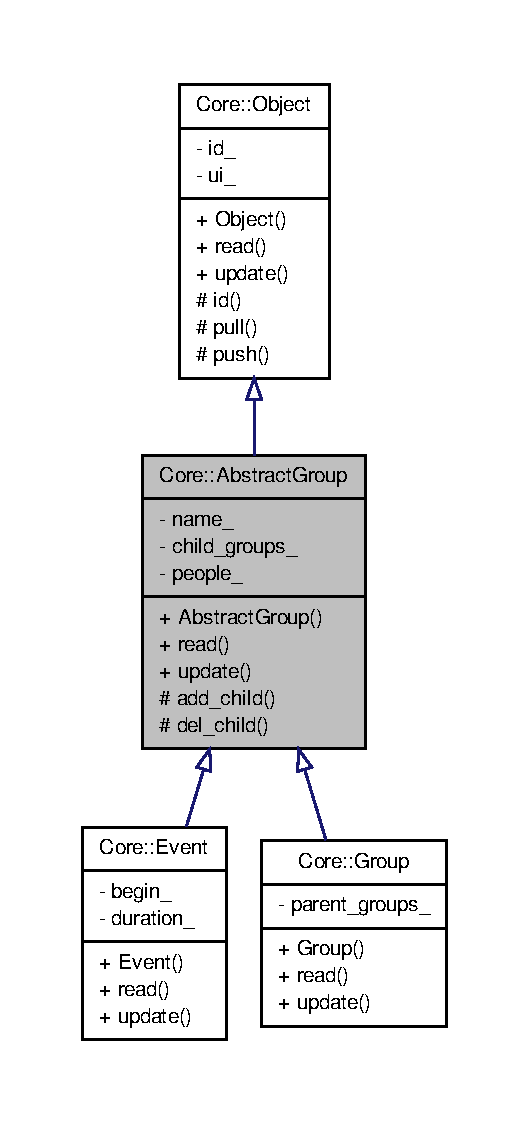
\includegraphics[width=254pt]{d2/d03/classCore_1_1AbstractGroup__inherit__graph}
\end{center}
\end{figure}


Collaboration diagram for Core::AbstractGroup:
\nopagebreak
\begin{figure}[H]
\begin{center}
\leavevmode
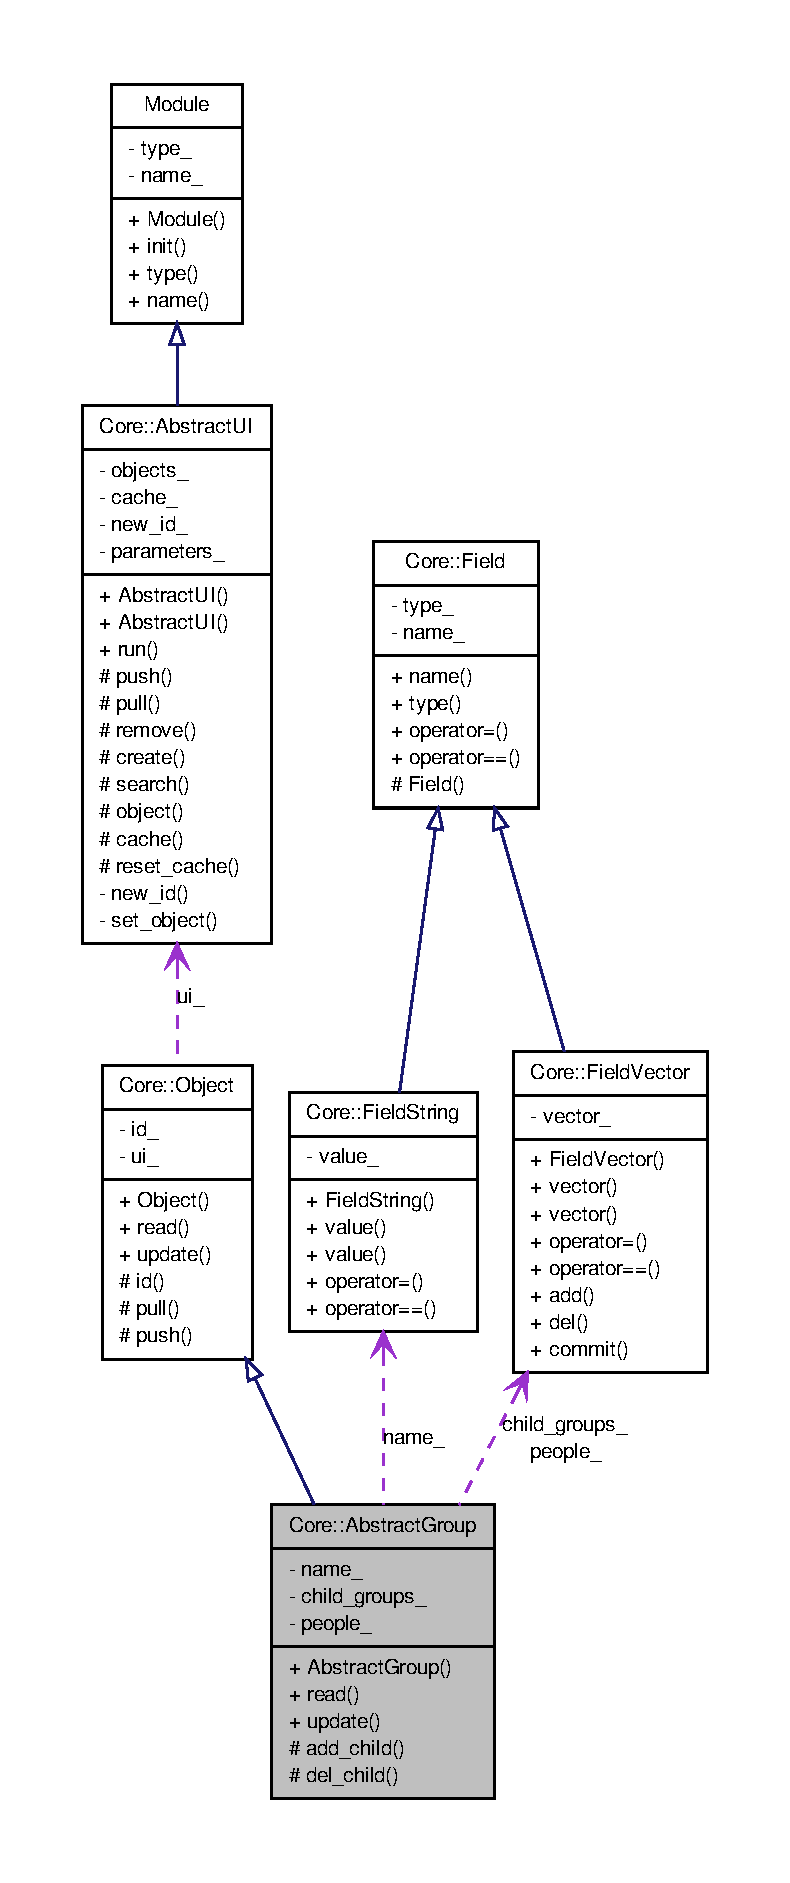
\includegraphics[height=600pt]{dd/dad/classCore_1_1AbstractGroup__coll__graph}
\end{center}
\end{figure}
\subsection*{Public Member Functions}
\begin{DoxyCompactItemize}
\item 
\hyperlink{classCore_1_1AbstractGroup_a413d72742d0f92f44615dba99e3430fd}{AbstractGroup} (const int id, \hyperlink{classCore_1_1AbstractUI}{AbstractUI} \&ui)  throw (std::bad\_\-cast)
\begin{DoxyCompactList}\small\item\em Constructor. \item\end{DoxyCompactList}\item 
virtual const \hyperlink{classCore_1_1Field}{Field} \& \hyperlink{classCore_1_1AbstractGroup_afd7a53d0bc49a5dbdc15505a686fca3d}{read} (const std::string \&name) const   throw (std::bad\_\-cast)
\item 
virtual void \hyperlink{classCore_1_1AbstractGroup_a397f639a0ee32efbc5a3ead8002745d5}{update} (const \hyperlink{classCore_1_1Field}{Field} \&field)  throw (std::bad\_\-cast)
\end{DoxyCompactItemize}
\subsection*{Protected Member Functions}
\begin{DoxyCompactItemize}
\item 
void \hyperlink{classCore_1_1AbstractGroup_aef90e91087aa5fcf4a94f0f2677f8f56}{add\_\-child} (\hyperlink{classCore_1_1AbstractGroup}{AbstractGroup} $\ast$group)
\begin{DoxyCompactList}\small\item\em Add child group to this one. \item\end{DoxyCompactList}\item 
void \hyperlink{classCore_1_1AbstractGroup_aa81866b9c414c24d25ca26311b4b4330}{del\_\-child} (\hyperlink{classCore_1_1AbstractGroup}{AbstractGroup} $\ast$group)
\begin{DoxyCompactList}\small\item\em Delete child group from this one. \item\end{DoxyCompactList}\end{DoxyCompactItemize}
\subsection*{Friends}
\begin{DoxyCompactItemize}
\item 
class \hyperlink{classCore_1_1AbstractGroup_a2697825715974a353728f0d4d5658112}{Group}
\end{DoxyCompactItemize}


\subsection{Detailed Description}
Base group functionality. You need to use it instead of \hyperlink{classCore_1_1Group}{Group} or \hyperlink{classCore_1_1Event}{Event} in most cases. This is a generalization of groups and events. It allows to work easy with them. It have not parent group as an \hyperlink{classCore_1_1Event}{Event}, but \hyperlink{classCore_1_1Group}{Group} have. 

\subsection{Constructor \& Destructor Documentation}
\hypertarget{classCore_1_1AbstractGroup_a413d72742d0f92f44615dba99e3430fd}{
\index{Core::AbstractGroup@{Core::AbstractGroup}!AbstractGroup@{AbstractGroup}}
\index{AbstractGroup@{AbstractGroup}!Core::AbstractGroup@{Core::AbstractGroup}}
\subsubsection[{AbstractGroup}]{\setlength{\rightskip}{0pt plus 5cm}AbstractGroup::AbstractGroup (
\begin{DoxyParamCaption}
\item[{const int}]{id, }
\item[{{\bf AbstractUI} \&}]{ui}
\end{DoxyParamCaption}
)  throw (std::bad\_\-cast)}}
\label{dd/d68/classCore_1_1AbstractGroup_a413d72742d0f92f44615dba99e3430fd}


Constructor. 


\begin{DoxyParams}[1]{Parameters}
\mbox{\tt in}  & {\em id} & AbstractUIs object`s identificator. \\
\hline
\mbox{\tt in}  & {\em ui} & Storage. \\
\hline
\end{DoxyParams}


\subsection{Member Function Documentation}
\hypertarget{classCore_1_1AbstractGroup_aef90e91087aa5fcf4a94f0f2677f8f56}{
\index{Core::AbstractGroup@{Core::AbstractGroup}!add\_\-child@{add\_\-child}}
\index{add\_\-child@{add\_\-child}!Core::AbstractGroup@{Core::AbstractGroup}}
\subsubsection[{add\_\-child}]{\setlength{\rightskip}{0pt plus 5cm}void AbstractGroup::add\_\-child (
\begin{DoxyParamCaption}
\item[{{\bf AbstractGroup} $\ast$}]{group}
\end{DoxyParamCaption}
)\hspace{0.3cm}{\ttfamily  \mbox{[}protected\mbox{]}}}}
\label{dd/d68/classCore_1_1AbstractGroup_aef90e91087aa5fcf4a94f0f2677f8f56}


Add child group to this one. 


\begin{DoxyParams}[1]{Parameters}
\mbox{\tt in}  & {\em group} & \hyperlink{classCore_1_1Group}{Group} to add. \\
\hline
\end{DoxyParams}


Here is the call graph for this function:
\nopagebreak
\begin{figure}[H]
\begin{center}
\leavevmode
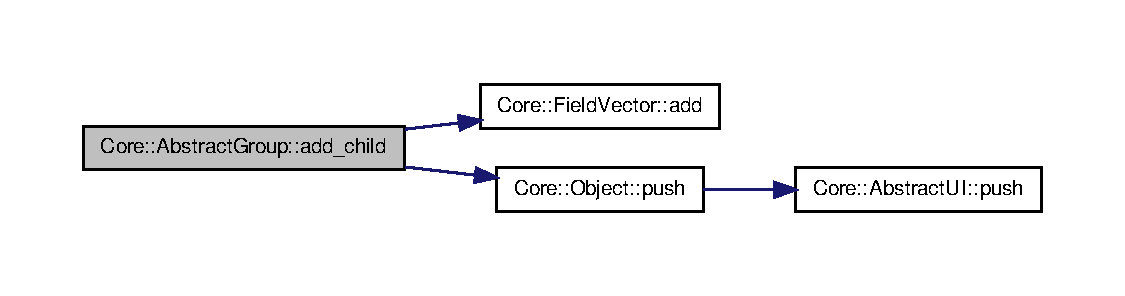
\includegraphics[width=400pt]{dd/d68/classCore_1_1AbstractGroup_aef90e91087aa5fcf4a94f0f2677f8f56_cgraph}
\end{center}
\end{figure}


\hypertarget{classCore_1_1AbstractGroup_aa81866b9c414c24d25ca26311b4b4330}{
\index{Core::AbstractGroup@{Core::AbstractGroup}!del\_\-child@{del\_\-child}}
\index{del\_\-child@{del\_\-child}!Core::AbstractGroup@{Core::AbstractGroup}}
\subsubsection[{del\_\-child}]{\setlength{\rightskip}{0pt plus 5cm}void AbstractGroup::del\_\-child (
\begin{DoxyParamCaption}
\item[{{\bf AbstractGroup} $\ast$}]{group}
\end{DoxyParamCaption}
)\hspace{0.3cm}{\ttfamily  \mbox{[}protected\mbox{]}}}}
\label{dd/d68/classCore_1_1AbstractGroup_aa81866b9c414c24d25ca26311b4b4330}


Delete child group from this one. 


\begin{DoxyParams}[1]{Parameters}
\mbox{\tt in}  & {\em group} & \hyperlink{classCore_1_1Group}{Group} to delete.  For use in \hyperlink{classCore_1_1Group_a9878d4ec0b02890502c6cff69da1e332}{Core::Group::update} method only.\\
\hline
\end{DoxyParams}
You must not use this method directly Use update methods instead. 

Here is the call graph for this function:
\nopagebreak
\begin{figure}[H]
\begin{center}
\leavevmode
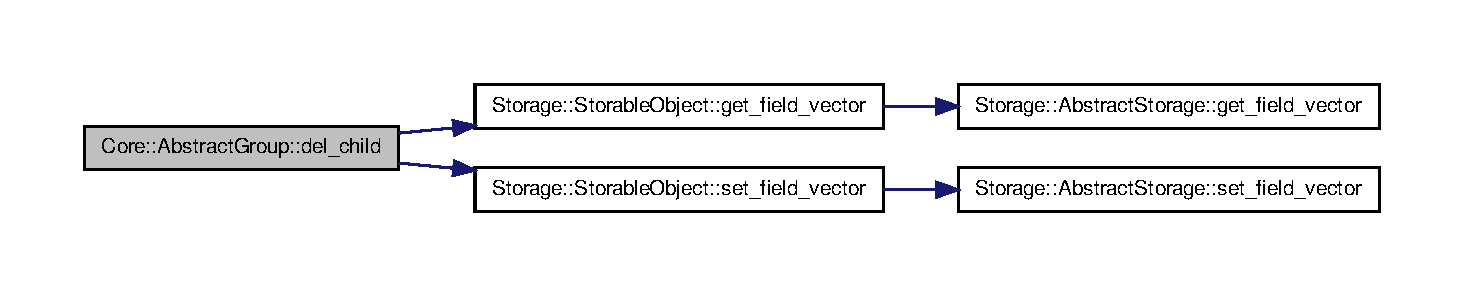
\includegraphics[width=400pt]{dd/d68/classCore_1_1AbstractGroup_aa81866b9c414c24d25ca26311b4b4330_cgraph}
\end{center}
\end{figure}


\hypertarget{classCore_1_1AbstractGroup_afd7a53d0bc49a5dbdc15505a686fca3d}{
\index{Core::AbstractGroup@{Core::AbstractGroup}!read@{read}}
\index{read@{read}!Core::AbstractGroup@{Core::AbstractGroup}}
\subsubsection[{read}]{\setlength{\rightskip}{0pt plus 5cm}const {\bf Field} \& AbstractGroup::read (
\begin{DoxyParamCaption}
\item[{const std::string \&}]{name}
\end{DoxyParamCaption}
) const  throw (std::bad\_\-cast)\hspace{0.3cm}{\ttfamily  \mbox{[}virtual\mbox{]}}}}
\label{dd/d68/classCore_1_1AbstractGroup_afd7a53d0bc49a5dbdc15505a686fca3d}
Get field of the object. 


\begin{DoxyParams}[1]{Parameters}
\mbox{\tt in}  & {\em name} & Name of the field to get. \\
\hline
\end{DoxyParams}
\begin{DoxyReturn}{Returns}
Corresponding field. 
\end{DoxyReturn}
 Get values of fields with those names: \char`\"{}name\char`\"{}, \char`\"{}people\char`\"{}, \char`\"{}child\_\-groups\char`\"{}.

Method returns object of \hyperlink{classCore_1_1FieldString}{Core::FieldString} or \hyperlink{classCore_1_1FieldVector}{Core::FieldVector} types. 

Implements \hyperlink{classCore_1_1Object_a90137d9981bd680bd395460e643c6560}{Core::Object}.



Reimplemented in \hyperlink{classCore_1_1Event_ac78ff90453b84d3342971772bba5c265}{Core::Event}, and \hyperlink{classCore_1_1Group_a0f4f5f00e11faeaaf09600d5b4943012}{Core::Group}.



Here is the caller graph for this function:
\nopagebreak
\begin{figure}[H]
\begin{center}
\leavevmode
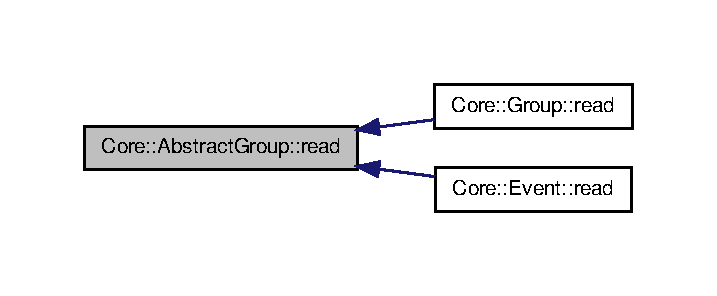
\includegraphics[width=344pt]{dd/d68/classCore_1_1AbstractGroup_afd7a53d0bc49a5dbdc15505a686fca3d_icgraph}
\end{center}
\end{figure}


\hypertarget{classCore_1_1AbstractGroup_a397f639a0ee32efbc5a3ead8002745d5}{
\index{Core::AbstractGroup@{Core::AbstractGroup}!update@{update}}
\index{update@{update}!Core::AbstractGroup@{Core::AbstractGroup}}
\subsubsection[{update}]{\setlength{\rightskip}{0pt plus 5cm}void AbstractGroup::update (
\begin{DoxyParamCaption}
\item[{const {\bf Field} \&}]{field}
\end{DoxyParamCaption}
)  throw (std::bad\_\-cast)\hspace{0.3cm}{\ttfamily  \mbox{[}virtual\mbox{]}}}}
\label{dd/d68/classCore_1_1AbstractGroup_a397f639a0ee32efbc5a3ead8002745d5}
Change field of the object. 


\begin{DoxyParams}[1]{Parameters}
\mbox{\tt in}  & {\em field} & \hyperlink{classCore_1_1Field}{Field} to change. \\
\hline
\end{DoxyParams}
 Change values of fields with those names: \char`\"{}name\char`\"{}, \char`\"{}people\char`\"{}, \char`\"{}child\_\-groups\char`\"{}.

Methods accepts object of \hyperlink{classCore_1_1FieldString}{Core::FieldString}, \hyperlink{classCore_1_1FieldLink}{Core::FieldLink} or \hyperlink{classCore_1_1FieldVector}{Core::FieldVector} types. 

Implements \hyperlink{classCore_1_1Object_a53328d659235e29f418ff4890cc3bdb3}{Core::Object}.



Reimplemented in \hyperlink{classCore_1_1Event_a8e147f35e8ee4fd0891a290424b098d3}{Core::Event}, and \hyperlink{classCore_1_1Group_a9878d4ec0b02890502c6cff69da1e332}{Core::Group}.



Here is the caller graph for this function:
\nopagebreak
\begin{figure}[H]
\begin{center}
\leavevmode
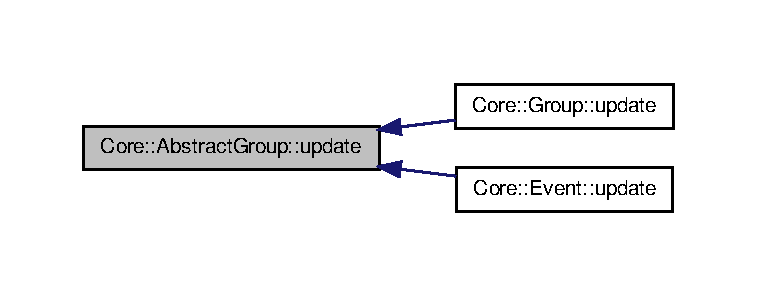
\includegraphics[width=364pt]{dd/d68/classCore_1_1AbstractGroup_a397f639a0ee32efbc5a3ead8002745d5_icgraph}
\end{center}
\end{figure}




\subsection{Friends And Related Function Documentation}
\hypertarget{classCore_1_1AbstractGroup_a2697825715974a353728f0d4d5658112}{
\index{Core::AbstractGroup@{Core::AbstractGroup}!Group@{Group}}
\index{Group@{Group}!Core::AbstractGroup@{Core::AbstractGroup}}
\subsubsection[{Group}]{\setlength{\rightskip}{0pt plus 5cm}friend class {\bf Group}\hspace{0.3cm}{\ttfamily  \mbox{[}friend\mbox{]}}}}
\label{dd/d68/classCore_1_1AbstractGroup_a2697825715974a353728f0d4d5658112}


The documentation for this class was generated from the following files:\begin{DoxyCompactItemize}
\item 
src/include/\hyperlink{abstractgroup_8h}{abstractgroup.h}\item 
src/core/\hyperlink{abstractgroup_8cpp}{abstractgroup.cpp}\end{DoxyCompactItemize}

\hypertarget{classCore_1_1AbstractUI}{
\section{Core::AbstractUI Class Reference}
\label{d1/d45/classCore_1_1AbstractUI}\index{Core::AbstractUI@{Core::AbstractUI}}
}


Interface for frontend modules.  




{\ttfamily \#include $<$abstractui.h$>$}



Inheritance diagram for Core::AbstractUI:
\nopagebreak
\begin{figure}[H]
\begin{center}
\leavevmode
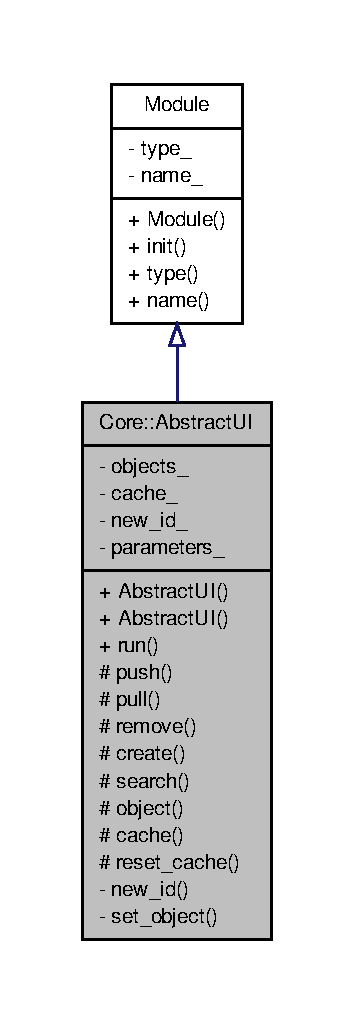
\includegraphics[width=170pt]{d4/d85/classCore_1_1AbstractUI__inherit__graph}
\end{center}
\end{figure}


Collaboration diagram for Core::AbstractUI:
\nopagebreak
\begin{figure}[H]
\begin{center}
\leavevmode
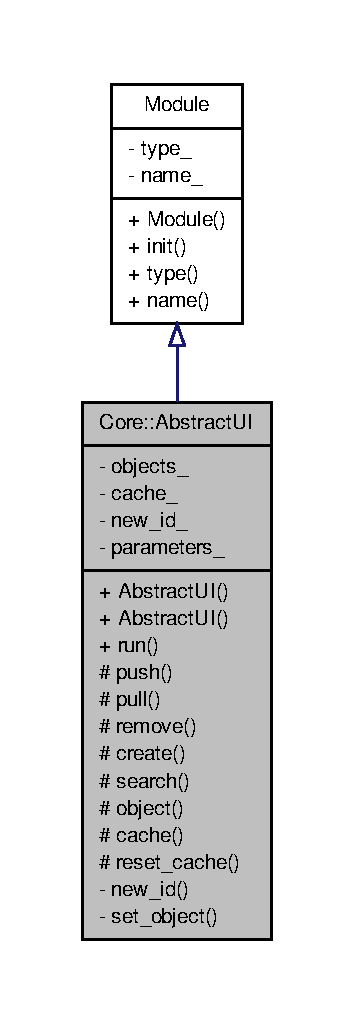
\includegraphics[width=170pt]{d0/d9b/classCore_1_1AbstractUI__coll__graph}
\end{center}
\end{figure}
\subsection*{Public Member Functions}
\begin{DoxyCompactItemize}
\item 
\hyperlink{classCore_1_1AbstractUI_a498c009d8806964b22d13ac2cf27479f}{AbstractUI} (const std::string \&name)
\begin{DoxyCompactList}\small\item\em constructor. \item\end{DoxyCompactList}\item 
\hyperlink{classCore_1_1AbstractUI_a92f84695ae72af96d9e5e3f024d2bafe}{AbstractUI} (std::fstream input\_\-storage, const std::string \&name)
\item 
virtual int \hyperlink{classCore_1_1AbstractUI_ac832b32700b97b1e0a6651efe7a1ce06}{run} ()=0
\begin{DoxyCompactList}\small\item\em Main method of frontend class. It is called from main. \item\end{DoxyCompactList}\end{DoxyCompactItemize}
\subsection*{Protected Member Functions}
\begin{DoxyCompactItemize}
\item 
void \hyperlink{classCore_1_1AbstractUI_a2744c5f015639a849c3f76dd7cc2656a}{push} (const int id, const \hyperlink{classCore_1_1Field}{Field} \&field)
\item 
const \hyperlink{classCore_1_1Field}{Field} \& \hyperlink{classCore_1_1AbstractUI_a2f70b789e482b7cf8a8b8574d29dc07b}{pull} (const std::string \&name) const   throw (std::bad\_\-cast)
\begin{DoxyCompactList}\small\item\em Load field with {\itshape name\/} of created object. \item\end{DoxyCompactList}\item 
void \hyperlink{classCore_1_1AbstractUI_abfdd0df1f1b2eeeab68536fa45d06c79}{remove} (\hyperlink{classCore_1_1Object}{Object} $\ast$object)
\item 
{\footnotesize template$<$class T $>$ }\\void \hyperlink{classCore_1_1AbstractUI_ac49885c7a9e25368e15172057f05d6a9}{create} (std::vector$<$ const \hyperlink{classCore_1_1Field}{Field} $>$ \&parameters)
\item 
void \hyperlink{classCore_1_1AbstractUI_aeffc2f4b846f5df74016a5bbed4f5549}{search} (const std::vector$<$ const \hyperlink{classCore_1_1Field}{Field} $\ast$ $>$ \&parameters)
\begin{DoxyCompactList}\small\item\em Search objects by some parameters. \item\end{DoxyCompactList}\item 
\hyperlink{classCore_1_1Object}{Object} $\ast$ \hyperlink{classCore_1_1AbstractUI_aa362757c2e56131d494986f34d31a5ad}{object} (const int id) const   throw (std::bad\_\-cast)
\begin{DoxyCompactList}\small\item\em Return object by id. \item\end{DoxyCompactList}\item 
std::vector$<$ \hyperlink{classCore_1_1Object}{Object} $\ast$ $>$ \& \hyperlink{classCore_1_1AbstractUI_afb9ec6d8636888b77cfcdc37713d5abc}{cache} ()
\item 
void \hyperlink{classCore_1_1AbstractUI_ade9be0dbb4b274ed6ef4d0d427152916}{reset\_\-cache} ()  throw ()
\begin{DoxyCompactList}\small\item\em Clears search cache. \item\end{DoxyCompactList}\end{DoxyCompactItemize}
\subsection*{Friends}
\begin{DoxyCompactItemize}
\item 
class \hyperlink{classCore_1_1AbstractUI_a0720b5f434e636e22a3ed34f847eec57}{Object}
\end{DoxyCompactItemize}


\subsection{Detailed Description}
Interface for frontend modules. 

\subsection{Constructor \& Destructor Documentation}
\hypertarget{classCore_1_1AbstractUI_a498c009d8806964b22d13ac2cf27479f}{
\index{Core::AbstractUI@{Core::AbstractUI}!AbstractUI@{AbstractUI}}
\index{AbstractUI@{AbstractUI}!Core::AbstractUI@{Core::AbstractUI}}
\subsubsection[{AbstractUI}]{\setlength{\rightskip}{0pt plus 5cm}Core::AbstractUI::AbstractUI (
\begin{DoxyParamCaption}
\item[{const std::string \&}]{name}
\end{DoxyParamCaption}
)\hspace{0.3cm}{\ttfamily  \mbox{[}inline\mbox{]}}}}
\label{d1/d45/classCore_1_1AbstractUI_a498c009d8806964b22d13ac2cf27479f}


constructor. 

$<$ 
\begin{DoxyParams}{Parameters}
{\em name} & Name of the frontend. \\
\hline
\end{DoxyParams}
\hypertarget{classCore_1_1AbstractUI_a92f84695ae72af96d9e5e3f024d2bafe}{
\index{Core::AbstractUI@{Core::AbstractUI}!AbstractUI@{AbstractUI}}
\index{AbstractUI@{AbstractUI}!Core::AbstractUI@{Core::AbstractUI}}
\subsubsection[{AbstractUI}]{\setlength{\rightskip}{0pt plus 5cm}AbstractUI::AbstractUI (
\begin{DoxyParamCaption}
\item[{std::fstream}]{input\_\-storage, }
\item[{const std::string \&}]{name}
\end{DoxyParamCaption}
)}}
\label{d1/d45/classCore_1_1AbstractUI_a92f84695ae72af96d9e5e3f024d2bafe}


\subsection{Member Function Documentation}
\hypertarget{classCore_1_1AbstractUI_afb9ec6d8636888b77cfcdc37713d5abc}{
\index{Core::AbstractUI@{Core::AbstractUI}!cache@{cache}}
\index{cache@{cache}!Core::AbstractUI@{Core::AbstractUI}}
\subsubsection[{cache}]{\setlength{\rightskip}{0pt plus 5cm}std::vector$<${\bf Object} $\ast$$>$\& Core::AbstractUI::cache (
\begin{DoxyParamCaption}
{}
\end{DoxyParamCaption}
)\hspace{0.3cm}{\ttfamily  \mbox{[}inline, protected\mbox{]}}}}
\label{d1/d45/classCore_1_1AbstractUI_afb9ec6d8636888b77cfcdc37713d5abc}
\hypertarget{classCore_1_1AbstractUI_ac49885c7a9e25368e15172057f05d6a9}{
\index{Core::AbstractUI@{Core::AbstractUI}!create@{create}}
\index{create@{create}!Core::AbstractUI@{Core::AbstractUI}}
\subsubsection[{create}]{\setlength{\rightskip}{0pt plus 5cm}template$<$class T $>$ void Core::AbstractUI::create (
\begin{DoxyParamCaption}
\item[{std::vector$<$ const {\bf Field} $>$ \&}]{parameters}
\end{DoxyParamCaption}
)\hspace{0.3cm}{\ttfamily  \mbox{[}inline, protected\mbox{]}}}}
\label{d1/d45/classCore_1_1AbstractUI_ac49885c7a9e25368e15172057f05d6a9}

\begin{DoxyParams}[1]{Parameters}
 & {\em parameters} & Create an object of the T type \\
\hline
\mbox{\tt in}  & {\em parameters} & new object`s data. \\
\hline
\end{DoxyParams}
\hypertarget{classCore_1_1AbstractUI_aa362757c2e56131d494986f34d31a5ad}{
\index{Core::AbstractUI@{Core::AbstractUI}!object@{object}}
\index{object@{object}!Core::AbstractUI@{Core::AbstractUI}}
\subsubsection[{object}]{\setlength{\rightskip}{0pt plus 5cm}{\bf Object}$\ast$ Core::AbstractUI::object (
\begin{DoxyParamCaption}
\item[{const int}]{id}
\end{DoxyParamCaption}
) const  throw (std::bad\_\-cast)\hspace{0.3cm}{\ttfamily  \mbox{[}inline, protected\mbox{]}}}}
\label{d1/d45/classCore_1_1AbstractUI_aa362757c2e56131d494986f34d31a5ad}


Return object by id. 

$<$ 
\begin{DoxyParams}[1]{Parameters}
\mbox{\tt in}  & {\em id} & \hyperlink{classCore_1_1Object}{Object} identificator. \\
\hline
\end{DoxyParams}
\begin{DoxyReturn}{Returns}
Requested object.
\end{DoxyReturn}
Use this method carefully. It can be moved to the protected or private on future. 

Here is the caller graph for this function:
\nopagebreak
\begin{figure}[H]
\begin{center}
\leavevmode
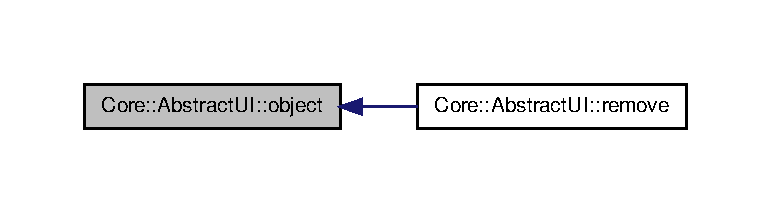
\includegraphics[width=370pt]{d1/d45/classCore_1_1AbstractUI_aa362757c2e56131d494986f34d31a5ad_icgraph}
\end{center}
\end{figure}


\hypertarget{classCore_1_1AbstractUI_a2f70b789e482b7cf8a8b8574d29dc07b}{
\index{Core::AbstractUI@{Core::AbstractUI}!pull@{pull}}
\index{pull@{pull}!Core::AbstractUI@{Core::AbstractUI}}
\subsubsection[{pull}]{\setlength{\rightskip}{0pt plus 5cm}const {\bf Field} \& AbstractUI::pull (
\begin{DoxyParamCaption}
\item[{const std::string \&}]{name}
\end{DoxyParamCaption}
) const  throw (std::bad\_\-cast)\hspace{0.3cm}{\ttfamily  \mbox{[}protected\mbox{]}}}}
\label{d1/d45/classCore_1_1AbstractUI_a2f70b789e482b7cf8a8b8574d29dc07b}


Load field with {\itshape name\/} of created object. 


\begin{DoxyParams}[1]{Parameters}
\mbox{\tt in}  & {\em name} & Name of the field. \\
\hline
\end{DoxyParams}
\begin{DoxyReturn}{Returns}
Corresponding field. 
\end{DoxyReturn}


Here is the caller graph for this function:
\nopagebreak
\begin{figure}[H]
\begin{center}
\leavevmode
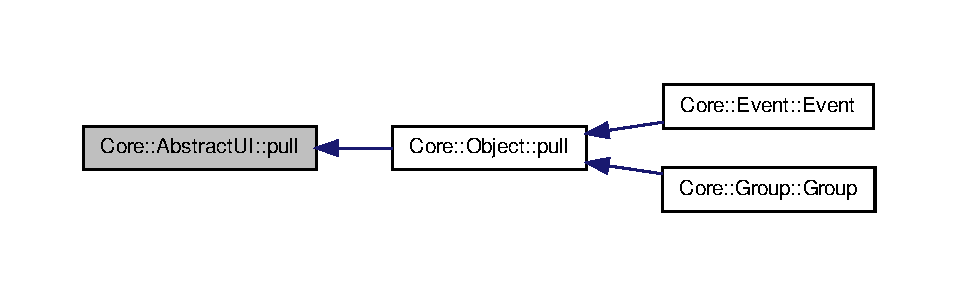
\includegraphics[width=400pt]{d1/d45/classCore_1_1AbstractUI_a2f70b789e482b7cf8a8b8574d29dc07b_icgraph}
\end{center}
\end{figure}


\hypertarget{classCore_1_1AbstractUI_a2744c5f015639a849c3f76dd7cc2656a}{
\index{Core::AbstractUI@{Core::AbstractUI}!push@{push}}
\index{push@{push}!Core::AbstractUI@{Core::AbstractUI}}
\subsubsection[{push}]{\setlength{\rightskip}{0pt plus 5cm}void Core::AbstractUI::push (
\begin{DoxyParamCaption}
\item[{const int}]{id, }
\item[{const {\bf Field} \&}]{field}
\end{DoxyParamCaption}
)\hspace{0.3cm}{\ttfamily  \mbox{[}inline, protected\mbox{]}}}}
\label{d1/d45/classCore_1_1AbstractUI_a2744c5f015639a849c3f76dd7cc2656a}

\begin{DoxyParams}[1]{Parameters}
 & {\em field} & Save {\itshape field\/} of object with {\itshape id\/} it hte database \\
\hline
\mbox{\tt in}  & {\em id} & Identificator of object. \\
\hline
\mbox{\tt in}  & {\em field} & \hyperlink{classCore_1_1Field}{Field} to save.\\
\hline
\end{DoxyParams}
TODO: Empty method. Write it, when create database class. 

Here is the caller graph for this function:
\nopagebreak
\begin{figure}[H]
\begin{center}
\leavevmode
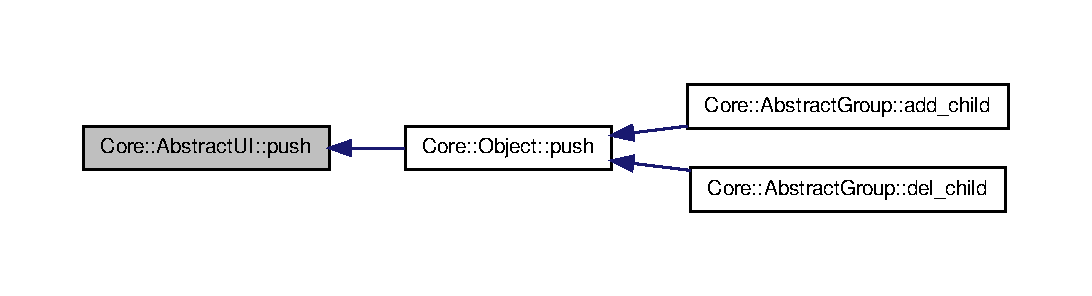
\includegraphics[width=400pt]{d1/d45/classCore_1_1AbstractUI_a2744c5f015639a849c3f76dd7cc2656a_icgraph}
\end{center}
\end{figure}


\hypertarget{classCore_1_1AbstractUI_abfdd0df1f1b2eeeab68536fa45d06c79}{
\index{Core::AbstractUI@{Core::AbstractUI}!remove@{remove}}
\index{remove@{remove}!Core::AbstractUI@{Core::AbstractUI}}
\subsubsection[{remove}]{\setlength{\rightskip}{0pt plus 5cm}void Core::AbstractUI::remove (
\begin{DoxyParamCaption}
\item[{{\bf Object} $\ast$}]{object}
\end{DoxyParamCaption}
)\hspace{0.3cm}{\ttfamily  \mbox{[}inline, protected\mbox{]}}}}
\label{d1/d45/classCore_1_1AbstractUI_abfdd0df1f1b2eeeab68536fa45d06c79}

\begin{DoxyParams}[1]{Parameters}
 & {\em object} & Remove object from the storage. \\
\hline
\mbox{\tt in}  & {\em object} & \hyperlink{classCore_1_1Object}{Object} to delete. \\
\hline
\end{DoxyParams}


Here is the call graph for this function:
\nopagebreak
\begin{figure}[H]
\begin{center}
\leavevmode
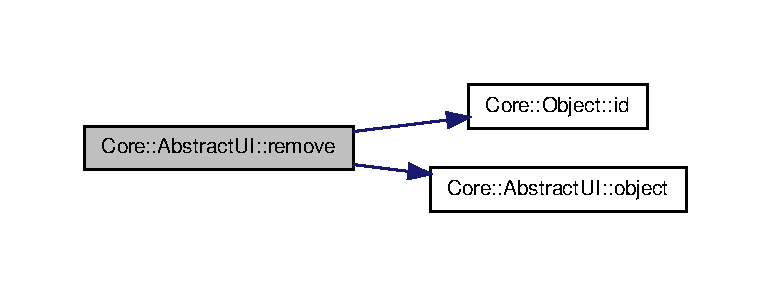
\includegraphics[width=370pt]{d1/d45/classCore_1_1AbstractUI_abfdd0df1f1b2eeeab68536fa45d06c79_cgraph}
\end{center}
\end{figure}


\hypertarget{classCore_1_1AbstractUI_ade9be0dbb4b274ed6ef4d0d427152916}{
\index{Core::AbstractUI@{Core::AbstractUI}!reset\_\-cache@{reset\_\-cache}}
\index{reset\_\-cache@{reset\_\-cache}!Core::AbstractUI@{Core::AbstractUI}}
\subsubsection[{reset\_\-cache}]{\setlength{\rightskip}{0pt plus 5cm}void Core::AbstractUI::reset\_\-cache (
\begin{DoxyParamCaption}
{}
\end{DoxyParamCaption}
)  throw ()\hspace{0.3cm}{\ttfamily  \mbox{[}inline, protected\mbox{]}}}}
\label{d1/d45/classCore_1_1AbstractUI_ade9be0dbb4b274ed6ef4d0d427152916}


Clears search cache. 

$<$ \hypertarget{classCore_1_1AbstractUI_ac832b32700b97b1e0a6651efe7a1ce06}{
\index{Core::AbstractUI@{Core::AbstractUI}!run@{run}}
\index{run@{run}!Core::AbstractUI@{Core::AbstractUI}}
\subsubsection[{run}]{\setlength{\rightskip}{0pt plus 5cm}virtual int Core::AbstractUI::run (
\begin{DoxyParamCaption}
{}
\end{DoxyParamCaption}
)\hspace{0.3cm}{\ttfamily  \mbox{[}pure virtual\mbox{]}}}}
\label{d1/d45/classCore_1_1AbstractUI_ac832b32700b97b1e0a6651efe7a1ce06}


Main method of frontend class. It is called from main. 

\begin{DoxyReturn}{Returns}
Program return code. 
\end{DoxyReturn}


Here is the caller graph for this function:
\nopagebreak
\begin{figure}[H]
\begin{center}
\leavevmode
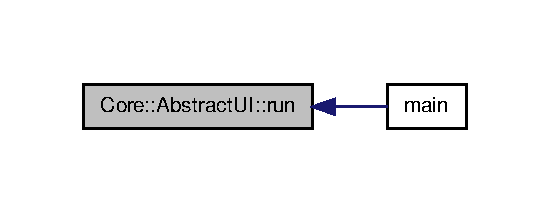
\includegraphics[width=264pt]{d1/d45/classCore_1_1AbstractUI_ac832b32700b97b1e0a6651efe7a1ce06_icgraph}
\end{center}
\end{figure}


\hypertarget{classCore_1_1AbstractUI_aeffc2f4b846f5df74016a5bbed4f5549}{
\index{Core::AbstractUI@{Core::AbstractUI}!search@{search}}
\index{search@{search}!Core::AbstractUI@{Core::AbstractUI}}
\subsubsection[{search}]{\setlength{\rightskip}{0pt plus 5cm}void AbstractUI::search (
\begin{DoxyParamCaption}
\item[{const std::vector$<$ const {\bf Field} $\ast$ $>$ \&}]{parameters}
\end{DoxyParamCaption}
)\hspace{0.3cm}{\ttfamily  \mbox{[}protected\mbox{]}}}}
\label{d1/d45/classCore_1_1AbstractUI_aeffc2f4b846f5df74016a5bbed4f5549}


Search objects by some parameters. 


\begin{DoxyParams}[1]{Parameters}
\mbox{\tt in}  & {\em parameters} & Search parameters.\\
\hline
\end{DoxyParams}
Parameters are connected by logical AND. If parameter have not got a name, search value by the any field of specified type. If value is empty that all objects will satisfied. 

\subsection{Friends And Related Function Documentation}
\hypertarget{classCore_1_1AbstractUI_a0720b5f434e636e22a3ed34f847eec57}{
\index{Core::AbstractUI@{Core::AbstractUI}!Object@{Object}}
\index{Object@{Object}!Core::AbstractUI@{Core::AbstractUI}}
\subsubsection[{Object}]{\setlength{\rightskip}{0pt plus 5cm}friend class {\bf Object}\hspace{0.3cm}{\ttfamily  \mbox{[}friend\mbox{]}}}}
\label{d1/d45/classCore_1_1AbstractUI_a0720b5f434e636e22a3ed34f847eec57}


The documentation for this class was generated from the following files:\begin{DoxyCompactItemize}
\item 
src/include/\hyperlink{abstractui_8h}{abstractui.h}\item 
src/core/\hyperlink{abstractui_8cpp}{abstractui.cpp}\end{DoxyCompactItemize}

\hypertarget{classDummyStorage}{
\section{DummyStorage Class Reference}
\label{d0/df2/classDummyStorage}\index{DummyStorage@{DummyStorage}}
}
Inheritance diagram for DummyStorage:\begin{figure}[H]
\begin{center}
\leavevmode
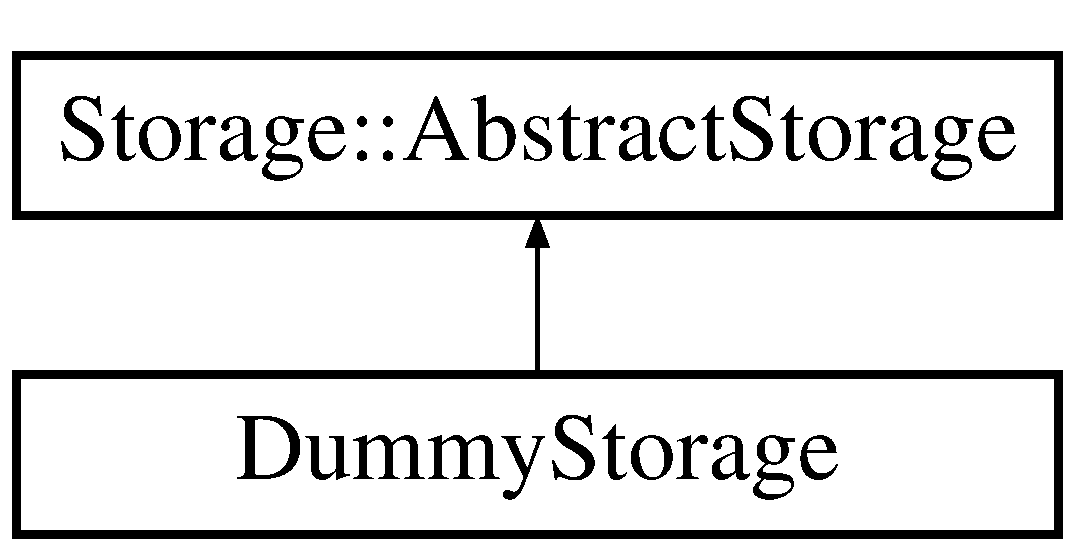
\includegraphics[height=2.000000cm]{d0/df2/classDummyStorage}
\end{center}
\end{figure}
\subsection*{Public Member Functions}
\begin{DoxyCompactItemize}
\item 
virtual std::vector$<$ \hyperlink{classStorage_1_1StorableObject}{Storage::StorableObject} $\ast$ $>$ $\ast$ \hyperlink{classDummyStorage_adea6bbcbaacaea1a728f09602d7c8d1d}{search} (std::vector$<$ \hyperlink{structStorage_1_1AbstractStorage_1_1Argument}{Argument} $\ast$ $>$ \&)
\begin{DoxyCompactList}\small\item\em Search objects by some parameters. \item\end{DoxyCompactList}\end{DoxyCompactItemize}
\subsection*{Protected Member Functions}
\begin{DoxyCompactItemize}
\item 
virtual const int \hyperlink{classDummyStorage_a275263eba82a652005292f01a120af8e}{get\_\-field\_\-int} (const int id, const std::string name) const   throw (std::bad\_\-cast)
\begin{DoxyCompactList}\small\item\em Return integer value of requested field. \item\end{DoxyCompactList}\item 
virtual const std::string \hyperlink{classDummyStorage_a410ef9d239193e25f830c49140e18293}{get\_\-field\_\-string} (const int id, const std::string name) const   throw (std::bad\_\-cast)
\begin{DoxyCompactList}\small\item\em Return string value of requested field. \item\end{DoxyCompactList}\item 
virtual const time\_\-t \hyperlink{classDummyStorage_a978ef9d688175e3739bb478f4c9b5313}{get\_\-field\_\-time} (const int id, const std::string name) const   throw (std::bad\_\-cast)
\begin{DoxyCompactList}\small\item\em Return time value of requested field. \item\end{DoxyCompactList}\item 
virtual const std::string \hyperlink{classDummyStorage_a1101739c23fbf79b009558553180ef1a}{get\_\-field\_\-enum} (const int id, const std::string name) const   throw (std::bad\_\-cast)
\begin{DoxyCompactList}\small\item\em Return enum value of requested field. \item\end{DoxyCompactList}\item 
virtual \hyperlink{classStorage_1_1StorableObject}{Storage::StorableObject} $\ast$ \hyperlink{classDummyStorage_a7135d171d9b83c2fbf72851fa9ea852a}{get\_\-field\_\-object} (const int id, const std::string name) const   throw (std::bad\_\-cast)
\begin{DoxyCompactList}\small\item\em Return object value of requested field. \item\end{DoxyCompactList}\item 
virtual const std::vector$<$ \hyperlink{classStorage_1_1StorableObject}{Storage::StorableObject} $\ast$ $>$ \hyperlink{classDummyStorage_afe36af3f3147027ebb6447192201c790}{get\_\-field\_\-vector} (const int id, const std::string name) const   throw (std::bad\_\-cast)
\begin{DoxyCompactList}\small\item\em Return vector value of requested field. \item\end{DoxyCompactList}\item 
virtual void \hyperlink{classDummyStorage_ab22488d00b8969af5356bc344672bd18}{set\_\-field} (const int id, const std::string name, const int value)  throw (std::bad\_\-cast)
\begin{DoxyCompactList}\small\item\em Set integer value of requested field. \item\end{DoxyCompactList}\item 
virtual void \hyperlink{classDummyStorage_aaa0d3249ea3207fae78253b191b80854}{set\_\-field} (const int id, const std::string name, const std::string value)  throw (std::bad\_\-cast)
\begin{DoxyCompactList}\small\item\em Set string value of requested field. \item\end{DoxyCompactList}\item 
virtual void \hyperlink{classDummyStorage_a51662a853e821fda1828e8756d58f1df}{set\_\-field} (const int id, const std::string name, const time\_\-t value)  throw (std::bad\_\-cast)
\begin{DoxyCompactList}\small\item\em Set time value of requested field. \item\end{DoxyCompactList}\item 
virtual void \hyperlink{classDummyStorage_a0655a6f7c822adbe174d1c7fe7c9ea34}{set\_\-field\_\-enum} (const int id, const std::string name, const std::string value)  throw (std::bad\_\-cast)
\begin{DoxyCompactList}\small\item\em Set enum value of requested field. \item\end{DoxyCompactList}\item 
virtual void \hyperlink{classDummyStorage_ae2e39a3cee22fd90790a7528f0c7ad59}{set\_\-field} (const int id, const std::string name, \hyperlink{classStorage_1_1StorableObject}{Storage::StorableObject} $\ast$value)  throw (std::bad\_\-cast)
\begin{DoxyCompactList}\small\item\em Set object value of requested field. \item\end{DoxyCompactList}\item 
virtual void \hyperlink{classDummyStorage_a6102ef89119b0ee1525439b3fd7043ce}{set\_\-field\_\-vector} (const int id, const std::string name, const std::vector$<$ \hyperlink{classStorage_1_1StorableObject}{Storage::StorableObject} $\ast$ $>$ value)  throw (std::bad\_\-cast)
\begin{DoxyCompactList}\small\item\em Set vector value of requested field. \item\end{DoxyCompactList}\end{DoxyCompactItemize}


\subsection{Member Function Documentation}
\hypertarget{classDummyStorage_a1101739c23fbf79b009558553180ef1a}{
\index{DummyStorage@{DummyStorage}!get\_\-field\_\-enum@{get\_\-field\_\-enum}}
\index{get\_\-field\_\-enum@{get\_\-field\_\-enum}!DummyStorage@{DummyStorage}}
\subsubsection[{get\_\-field\_\-enum}]{\setlength{\rightskip}{0pt plus 5cm}virtual const std::string DummyStorage::get\_\-field\_\-enum (
\begin{DoxyParamCaption}
\item[{const int}]{id, }
\item[{const std::string}]{field}
\end{DoxyParamCaption}
) const  throw (std::bad\_\-cast)\hspace{0.3cm}{\ttfamily  \mbox{[}inline, protected, virtual\mbox{]}}}}
\label{d0/df2/classDummyStorage_a1101739c23fbf79b009558553180ef1a}


Return enum value of requested field. 


\begin{DoxyParams}[1]{Parameters}
\mbox{\tt in}  & {\em id} & Object identificator. \\
\hline
\mbox{\tt in}  & {\em field} & Field name. \\
\hline
\end{DoxyParams}
\begin{DoxyReturn}{Returns}
requested value.
\end{DoxyReturn}
This method must be realized in inherited classes. Throw an std::bad\_\-cast exception if requested field does not exists or keeped in another type. 

Implements \hyperlink{classStorage_1_1AbstractStorage_acd7e88a005b6873632c7f20245e5f3f7}{Storage::AbstractStorage}.

\hypertarget{classDummyStorage_a275263eba82a652005292f01a120af8e}{
\index{DummyStorage@{DummyStorage}!get\_\-field\_\-int@{get\_\-field\_\-int}}
\index{get\_\-field\_\-int@{get\_\-field\_\-int}!DummyStorage@{DummyStorage}}
\subsubsection[{get\_\-field\_\-int}]{\setlength{\rightskip}{0pt plus 5cm}virtual const int DummyStorage::get\_\-field\_\-int (
\begin{DoxyParamCaption}
\item[{const int}]{id, }
\item[{const std::string}]{field}
\end{DoxyParamCaption}
) const  throw (std::bad\_\-cast)\hspace{0.3cm}{\ttfamily  \mbox{[}inline, protected, virtual\mbox{]}}}}
\label{d0/df2/classDummyStorage_a275263eba82a652005292f01a120af8e}


Return integer value of requested field. 


\begin{DoxyParams}[1]{Parameters}
\mbox{\tt in}  & {\em id} & Object identificator. \\
\hline
\mbox{\tt in}  & {\em field} & Field name. \\
\hline
\end{DoxyParams}
\begin{DoxyReturn}{Returns}
requested value.
\end{DoxyReturn}
This method must be realized in inherited classes. Throw an std::bad\_\-cast exception if requested field does not exists or keeped in another type. 

Implements \hyperlink{classStorage_1_1AbstractStorage_a80a7e4ab87a0326aa8b5571b09d55eaa}{Storage::AbstractStorage}.

\hypertarget{classDummyStorage_a7135d171d9b83c2fbf72851fa9ea852a}{
\index{DummyStorage@{DummyStorage}!get\_\-field\_\-object@{get\_\-field\_\-object}}
\index{get\_\-field\_\-object@{get\_\-field\_\-object}!DummyStorage@{DummyStorage}}
\subsubsection[{get\_\-field\_\-object}]{\setlength{\rightskip}{0pt plus 5cm}virtual {\bf Storage::StorableObject}$\ast$ DummyStorage::get\_\-field\_\-object (
\begin{DoxyParamCaption}
\item[{const int}]{id, }
\item[{const std::string}]{field}
\end{DoxyParamCaption}
) const  throw (std::bad\_\-cast)\hspace{0.3cm}{\ttfamily  \mbox{[}inline, protected, virtual\mbox{]}}}}
\label{d0/df2/classDummyStorage_a7135d171d9b83c2fbf72851fa9ea852a}


Return object value of requested field. 


\begin{DoxyParams}[1]{Parameters}
\mbox{\tt in}  & {\em id} & Object identificator. \\
\hline
\mbox{\tt in}  & {\em field} & Field name. \\
\hline
\end{DoxyParams}
\begin{DoxyReturn}{Returns}
requested value.
\end{DoxyReturn}
This method must be realized in inherited classes. Throw an std::bad\_\-cast exception if requested field does not exists or keeped in another type. 

Implements \hyperlink{classStorage_1_1AbstractStorage_aaff107d1f51e456f26c03861beb0fff7}{Storage::AbstractStorage}.

\hypertarget{classDummyStorage_a410ef9d239193e25f830c49140e18293}{
\index{DummyStorage@{DummyStorage}!get\_\-field\_\-string@{get\_\-field\_\-string}}
\index{get\_\-field\_\-string@{get\_\-field\_\-string}!DummyStorage@{DummyStorage}}
\subsubsection[{get\_\-field\_\-string}]{\setlength{\rightskip}{0pt plus 5cm}virtual const std::string DummyStorage::get\_\-field\_\-string (
\begin{DoxyParamCaption}
\item[{const int}]{id, }
\item[{const std::string}]{field}
\end{DoxyParamCaption}
) const  throw (std::bad\_\-cast)\hspace{0.3cm}{\ttfamily  \mbox{[}inline, protected, virtual\mbox{]}}}}
\label{d0/df2/classDummyStorage_a410ef9d239193e25f830c49140e18293}


Return string value of requested field. 


\begin{DoxyParams}[1]{Parameters}
\mbox{\tt in}  & {\em id} & Object identificator. \\
\hline
\mbox{\tt in}  & {\em field} & Field name. \\
\hline
\end{DoxyParams}
\begin{DoxyReturn}{Returns}
requested value.
\end{DoxyReturn}
This method must be realized in inherited classes. Throw an std::bad\_\-cast exception if requested field does not exists or keeped in another type. 

Implements \hyperlink{classStorage_1_1AbstractStorage_ad12a3abb791ef5a696196c28e643ec22}{Storage::AbstractStorage}.

\hypertarget{classDummyStorage_a978ef9d688175e3739bb478f4c9b5313}{
\index{DummyStorage@{DummyStorage}!get\_\-field\_\-time@{get\_\-field\_\-time}}
\index{get\_\-field\_\-time@{get\_\-field\_\-time}!DummyStorage@{DummyStorage}}
\subsubsection[{get\_\-field\_\-time}]{\setlength{\rightskip}{0pt plus 5cm}virtual const time\_\-t DummyStorage::get\_\-field\_\-time (
\begin{DoxyParamCaption}
\item[{const int}]{id, }
\item[{const std::string}]{field}
\end{DoxyParamCaption}
) const  throw (std::bad\_\-cast)\hspace{0.3cm}{\ttfamily  \mbox{[}inline, protected, virtual\mbox{]}}}}
\label{d0/df2/classDummyStorage_a978ef9d688175e3739bb478f4c9b5313}


Return time value of requested field. 


\begin{DoxyParams}[1]{Parameters}
\mbox{\tt in}  & {\em id} & Object identificator. \\
\hline
\mbox{\tt in}  & {\em field} & Field name. \\
\hline
\end{DoxyParams}
\begin{DoxyReturn}{Returns}
requested value.
\end{DoxyReturn}
This method must be realized in inherited classes. Throw an std::bad\_\-cast exception if requested field does not exists or keeped in another type. 

Implements \hyperlink{classStorage_1_1AbstractStorage_a87fe8d51934ab2403758d905ef313272}{Storage::AbstractStorage}.

\hypertarget{classDummyStorage_afe36af3f3147027ebb6447192201c790}{
\index{DummyStorage@{DummyStorage}!get\_\-field\_\-vector@{get\_\-field\_\-vector}}
\index{get\_\-field\_\-vector@{get\_\-field\_\-vector}!DummyStorage@{DummyStorage}}
\subsubsection[{get\_\-field\_\-vector}]{\setlength{\rightskip}{0pt plus 5cm}virtual const std::vector$<${\bf Storage::StorableObject} $\ast$$>$ DummyStorage::get\_\-field\_\-vector (
\begin{DoxyParamCaption}
\item[{const int}]{id, }
\item[{const std::string}]{field}
\end{DoxyParamCaption}
) const  throw (std::bad\_\-cast)\hspace{0.3cm}{\ttfamily  \mbox{[}inline, protected, virtual\mbox{]}}}}
\label{d0/df2/classDummyStorage_afe36af3f3147027ebb6447192201c790}


Return vector value of requested field. 


\begin{DoxyParams}[1]{Parameters}
\mbox{\tt in}  & {\em id} & Object identificator. \\
\hline
\mbox{\tt in}  & {\em field} & Field name. \\
\hline
\end{DoxyParams}
\begin{DoxyReturn}{Returns}
requested value.
\end{DoxyReturn}
This method must be realized in inherited classes. Throw an std::bad\_\-cast exception if requested field does not exists or keeped in another type. 

Implements \hyperlink{classStorage_1_1AbstractStorage_ae7c30697d68dc9d7de595388030d8e10}{Storage::AbstractStorage}.

\hypertarget{classDummyStorage_adea6bbcbaacaea1a728f09602d7c8d1d}{
\index{DummyStorage@{DummyStorage}!search@{search}}
\index{search@{search}!DummyStorage@{DummyStorage}}
\subsubsection[{search}]{\setlength{\rightskip}{0pt plus 5cm}virtual std::vector$<${\bf Storage::StorableObject} $\ast$$>$$\ast$ DummyStorage::search (
\begin{DoxyParamCaption}
\item[{std::vector$<$ {\bf Argument} $\ast$ $>$ \&}]{parameters}
\end{DoxyParamCaption}
)\hspace{0.3cm}{\ttfamily  \mbox{[}inline, virtual\mbox{]}}}}
\label{d0/df2/classDummyStorage_adea6bbcbaacaea1a728f09602d7c8d1d}


Search objects by some parameters. 


\begin{DoxyParams}[1]{Parameters}
\mbox{\tt in}  & {\em parameters} & Search parameters. \\
\hline
\end{DoxyParams}
\begin{DoxyReturn}{Returns}
Vector of found objects.
\end{DoxyReturn}
Parameters are connected by logical AND. If parameter have not got a name, search value by the any field of specified type. If value is empty that all objects will satisfied. 

Implements \hyperlink{classStorage_1_1AbstractStorage_a9304eea8cd6fffd77b1ccd26f85a061c}{Storage::AbstractStorage}.

\hypertarget{classDummyStorage_ab22488d00b8969af5356bc344672bd18}{
\index{DummyStorage@{DummyStorage}!set\_\-field@{set\_\-field}}
\index{set\_\-field@{set\_\-field}!DummyStorage@{DummyStorage}}
\subsubsection[{set\_\-field}]{\setlength{\rightskip}{0pt plus 5cm}virtual void DummyStorage::set\_\-field (
\begin{DoxyParamCaption}
\item[{const int}]{id, }
\item[{const std::string}]{field, }
\item[{const int}]{value}
\end{DoxyParamCaption}
)  throw (std::bad\_\-cast)\hspace{0.3cm}{\ttfamily  \mbox{[}inline, protected, virtual\mbox{]}}}}
\label{d0/df2/classDummyStorage_ab22488d00b8969af5356bc344672bd18}


Set integer value of requested field. 


\begin{DoxyParams}[1]{Parameters}
\mbox{\tt in}  & {\em id} & Object identificator. \\
\hline
\mbox{\tt in}  & {\em field} & Field name. \\
\hline
\mbox{\tt in}  & {\em value} & New value.\\
\hline
\end{DoxyParams}
This method must be realized in inherited classes. Throw an std::bad\_\-cast exception if requested field keeped in another type. 

Implements \hyperlink{classStorage_1_1AbstractStorage_acdd090d0beb6a8241914e7d78a7f2c0c}{Storage::AbstractStorage}.

\hypertarget{classDummyStorage_aaa0d3249ea3207fae78253b191b80854}{
\index{DummyStorage@{DummyStorage}!set\_\-field@{set\_\-field}}
\index{set\_\-field@{set\_\-field}!DummyStorage@{DummyStorage}}
\subsubsection[{set\_\-field}]{\setlength{\rightskip}{0pt plus 5cm}virtual void DummyStorage::set\_\-field (
\begin{DoxyParamCaption}
\item[{const int}]{id, }
\item[{const std::string}]{field, }
\item[{const std::string}]{value}
\end{DoxyParamCaption}
)  throw (std::bad\_\-cast)\hspace{0.3cm}{\ttfamily  \mbox{[}inline, protected, virtual\mbox{]}}}}
\label{d0/df2/classDummyStorage_aaa0d3249ea3207fae78253b191b80854}


Set string value of requested field. 


\begin{DoxyParams}[1]{Parameters}
\mbox{\tt in}  & {\em id} & Object identificator. \\
\hline
\mbox{\tt in}  & {\em field} & Field name. \\
\hline
\mbox{\tt in}  & {\em value} & New value.\\
\hline
\end{DoxyParams}
This method must be realized in inherited classes. Throw an std::bad\_\-cast exception if requested field keeped in another type. 

Implements \hyperlink{classStorage_1_1AbstractStorage_ae5ee00e647f121b68ebada0f094058bc}{Storage::AbstractStorage}.

\hypertarget{classDummyStorage_ae2e39a3cee22fd90790a7528f0c7ad59}{
\index{DummyStorage@{DummyStorage}!set\_\-field@{set\_\-field}}
\index{set\_\-field@{set\_\-field}!DummyStorage@{DummyStorage}}
\subsubsection[{set\_\-field}]{\setlength{\rightskip}{0pt plus 5cm}virtual void DummyStorage::set\_\-field (
\begin{DoxyParamCaption}
\item[{const int}]{id, }
\item[{const std::string}]{field, }
\item[{{\bf Storage::StorableObject} $\ast$}]{value}
\end{DoxyParamCaption}
)  throw (std::bad\_\-cast)\hspace{0.3cm}{\ttfamily  \mbox{[}inline, protected, virtual\mbox{]}}}}
\label{d0/df2/classDummyStorage_ae2e39a3cee22fd90790a7528f0c7ad59}


Set object value of requested field. 


\begin{DoxyParams}[1]{Parameters}
\mbox{\tt in}  & {\em id} & Object identificator. \\
\hline
\mbox{\tt in}  & {\em field} & Field name. \\
\hline
\mbox{\tt in}  & {\em value} & New value.\\
\hline
\end{DoxyParams}
This method must be realized in inherited classes. Throw an std::bad\_\-cast exception if requested field keeped in another type. 

Implements \hyperlink{classStorage_1_1AbstractStorage_a7ef9f70b3fcbaa2863de2be695dc77c1}{Storage::AbstractStorage}.

\hypertarget{classDummyStorage_a51662a853e821fda1828e8756d58f1df}{
\index{DummyStorage@{DummyStorage}!set\_\-field@{set\_\-field}}
\index{set\_\-field@{set\_\-field}!DummyStorage@{DummyStorage}}
\subsubsection[{set\_\-field}]{\setlength{\rightskip}{0pt plus 5cm}virtual void DummyStorage::set\_\-field (
\begin{DoxyParamCaption}
\item[{const int}]{id, }
\item[{const std::string}]{field, }
\item[{const time\_\-t}]{value}
\end{DoxyParamCaption}
)  throw (std::bad\_\-cast)\hspace{0.3cm}{\ttfamily  \mbox{[}inline, protected, virtual\mbox{]}}}}
\label{d0/df2/classDummyStorage_a51662a853e821fda1828e8756d58f1df}


Set time value of requested field. 


\begin{DoxyParams}[1]{Parameters}
\mbox{\tt in}  & {\em id} & Object identificator. \\
\hline
\mbox{\tt in}  & {\em field} & Field name. \\
\hline
\mbox{\tt in}  & {\em value} & New value.\\
\hline
\end{DoxyParams}
This method must be realized in inherited classes. Throw an std::bad\_\-cast exception if requested field keeped in another type. 

Implements \hyperlink{classStorage_1_1AbstractStorage_a50ee4a829bc067a9291a11aa99ec0f16}{Storage::AbstractStorage}.

\hypertarget{classDummyStorage_a0655a6f7c822adbe174d1c7fe7c9ea34}{
\index{DummyStorage@{DummyStorage}!set\_\-field\_\-enum@{set\_\-field\_\-enum}}
\index{set\_\-field\_\-enum@{set\_\-field\_\-enum}!DummyStorage@{DummyStorage}}
\subsubsection[{set\_\-field\_\-enum}]{\setlength{\rightskip}{0pt plus 5cm}virtual void DummyStorage::set\_\-field\_\-enum (
\begin{DoxyParamCaption}
\item[{const int}]{id, }
\item[{const std::string}]{field, }
\item[{const std::string}]{value}
\end{DoxyParamCaption}
)  throw (std::bad\_\-cast)\hspace{0.3cm}{\ttfamily  \mbox{[}inline, protected, virtual\mbox{]}}}}
\label{d0/df2/classDummyStorage_a0655a6f7c822adbe174d1c7fe7c9ea34}


Set enum value of requested field. 


\begin{DoxyParams}[1]{Parameters}
\mbox{\tt in}  & {\em id} & Object identificator. \\
\hline
\mbox{\tt in}  & {\em field} & Field name. \\
\hline
\mbox{\tt in}  & {\em value} & New value.\\
\hline
\end{DoxyParams}
This method must be realized in inherited classes. Throw an std::bad\_\-cast exception if requested field keeped in another type. 

Implements \hyperlink{classStorage_1_1AbstractStorage_a50925678c74c09acd8549a541fdbbe9f}{Storage::AbstractStorage}.

\hypertarget{classDummyStorage_a6102ef89119b0ee1525439b3fd7043ce}{
\index{DummyStorage@{DummyStorage}!set\_\-field\_\-vector@{set\_\-field\_\-vector}}
\index{set\_\-field\_\-vector@{set\_\-field\_\-vector}!DummyStorage@{DummyStorage}}
\subsubsection[{set\_\-field\_\-vector}]{\setlength{\rightskip}{0pt plus 5cm}virtual void DummyStorage::set\_\-field\_\-vector (
\begin{DoxyParamCaption}
\item[{const int}]{id, }
\item[{const std::string}]{field, }
\item[{const std::vector$<$ {\bf Storage::StorableObject} $\ast$ $>$}]{vector}
\end{DoxyParamCaption}
)  throw (std::bad\_\-cast)\hspace{0.3cm}{\ttfamily  \mbox{[}inline, protected, virtual\mbox{]}}}}
\label{d0/df2/classDummyStorage_a6102ef89119b0ee1525439b3fd7043ce}


Set vector value of requested field. 


\begin{DoxyParams}[1]{Parameters}
\mbox{\tt in}  & {\em id} & Object identificator. \\
\hline
\mbox{\tt in}  & {\em field} & Field name.  \mbox{[}in\mbox{]} value New value.\\
\hline
\end{DoxyParams}
This method must be realized in inherited classes. Throw an std::bad\_\-cast exception if requested field keeped in another type. 

Implements \hyperlink{classStorage_1_1AbstractStorage_a24af03b9a68ace199b0a6fa812abad39}{Storage::AbstractStorage}.



The documentation for this class was generated from the following file:\begin{DoxyCompactItemize}
\item 
src/tests/\hyperlink{model__classes__are__real_8cpp}{model\_\-classes\_\-are\_\-real.cpp}\end{DoxyCompactItemize}

\hypertarget{classCore_1_1Event}{
\section{Core::Event Class Reference}
\label{d9/d42/classCore_1_1Event}\index{Core::Event@{Core::Event}}
}


{\ttfamily \#include $<$event.h$>$}

Inheritance diagram for Core::Event:\begin{figure}[H]
\begin{center}
\leavevmode
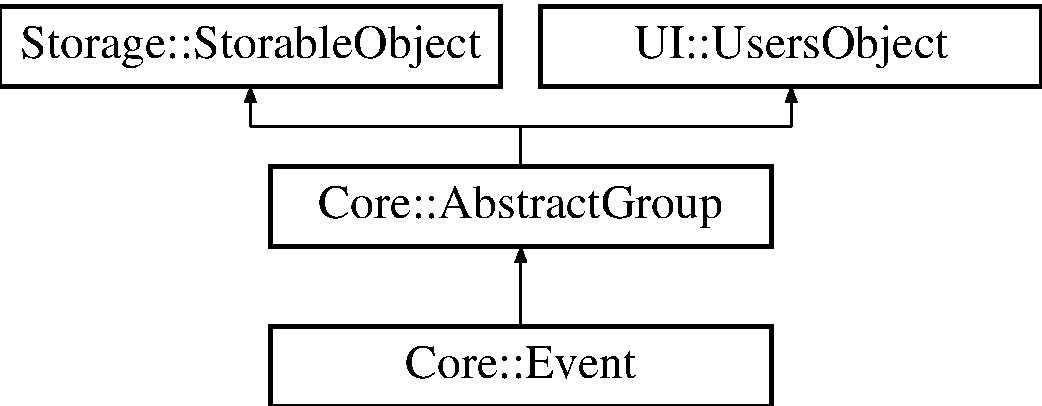
\includegraphics[height=3.000000cm]{d9/d42/classCore_1_1Event}
\end{center}
\end{figure}
\subsection*{Public Member Functions}
\begin{DoxyCompactItemize}
\item 
\hyperlink{classCore_1_1Event_a067e37070ea0fa9b39d7d1171c2f9a2d}{Event} (const int id, \hyperlink{classStorage_1_1AbstractStorage}{Storage::AbstractStorage} \&storage)
\item 
\hyperlink{classCore_1_1Event_aa4a154dde2ab0f1e011fc2f41909cb43}{Event} (const int id, \hyperlink{classStorage_1_1AbstractStorage}{Storage::AbstractStorage} \&storage, const std::string name, const time\_\-t begin, const time\_\-t duration)
\item 
const time\_\-t \hyperlink{classCore_1_1Event_a829b19b781b4d5989928c021b3a3553a}{begin} () const 
\item 
const time\_\-t \hyperlink{classCore_1_1Event_ad83a2109fa632352f63adfdafe2dc86f}{duration} () const 
\item 
const time\_\-t \hyperlink{classCore_1_1Event_af83b91c07834359638a4f7473abad5c5}{end} () const 
\item 
virtual const std::string \hyperlink{classCore_1_1Event_a8dd94bcb05cb3c5ef065fa204cd724f9}{read} () const 
\begin{DoxyCompactList}\small\item\em Returns full object information. \item\end{DoxyCompactList}\item 
virtual const time\_\-t \hyperlink{classCore_1_1Event_a4977832cb03001d8afe46bcddc60ce1a}{read\_\-time} (const std::string name) const   throw (std::bad\_\-cast)
\begin{DoxyCompactList}\small\item\em Return time value of requested field. \item\end{DoxyCompactList}\item 
virtual void \hyperlink{classCore_1_1Event_aaa4b9def6b65cc896e0054210b2d5dae}{update} (const std::string name, const time\_\-t value)  throw (std::bad\_\-cast)
\begin{DoxyCompactList}\small\item\em change current time value of field. \item\end{DoxyCompactList}\item 
virtual void \hyperlink{classCore_1_1Event_a308ae7ad334b8c9a166dc57cfd6a0524}{update} (\hyperlink{classUI_1_1UsersObject}{UI::UsersObject} $\ast$object, const bool linked)  throw (std::bad\_\-cast)
\begin{DoxyCompactList}\small\item\em change current link value of field. \item\end{DoxyCompactList}\end{DoxyCompactItemize}
\subsection*{Protected Member Functions}
\begin{DoxyCompactItemize}
\item 
virtual void \hyperlink{classCore_1_1Event_a6dbea64bf650e7e36d55539cf59a66e7}{save} ()
\begin{DoxyCompactList}\small\item\em Method to save all data in the storage. \item\end{DoxyCompactList}\item 
virtual void \hyperlink{classCore_1_1Event_a63462f7c20234f5c7f18e9c5e19d72b9}{load} ()
\begin{DoxyCompactList}\small\item\em Method to load all data from the storage. \item\end{DoxyCompactList}\end{DoxyCompactItemize}


\subsection{Constructor \& Destructor Documentation}
\hypertarget{classCore_1_1Event_a067e37070ea0fa9b39d7d1171c2f9a2d}{
\index{Core::Event@{Core::Event}!Event@{Event}}
\index{Event@{Event}!Core::Event@{Core::Event}}
\subsubsection[{Event}]{\setlength{\rightskip}{0pt plus 5cm}Core::Event::Event (
\begin{DoxyParamCaption}
\item[{const int}]{id, }
\item[{{\bf Storage::AbstractStorage} \&}]{storage}
\end{DoxyParamCaption}
)\hspace{0.3cm}{\ttfamily  \mbox{[}inline\mbox{]}}}}
\label{d9/d42/classCore_1_1Event_a067e37070ea0fa9b39d7d1171c2f9a2d}
\hypertarget{classCore_1_1Event_aa4a154dde2ab0f1e011fc2f41909cb43}{
\index{Core::Event@{Core::Event}!Event@{Event}}
\index{Event@{Event}!Core::Event@{Core::Event}}
\subsubsection[{Event}]{\setlength{\rightskip}{0pt plus 5cm}Core::Event::Event (
\begin{DoxyParamCaption}
\item[{const int}]{id, }
\item[{{\bf Storage::AbstractStorage} \&}]{storage, }
\item[{const std::string}]{name, }
\item[{const time\_\-t}]{begin, }
\item[{const time\_\-t}]{duration}
\end{DoxyParamCaption}
)\hspace{0.3cm}{\ttfamily  \mbox{[}inline\mbox{]}}}}
\label{d9/d42/classCore_1_1Event_aa4a154dde2ab0f1e011fc2f41909cb43}


\subsection{Member Function Documentation}
\hypertarget{classCore_1_1Event_a829b19b781b4d5989928c021b3a3553a}{
\index{Core::Event@{Core::Event}!begin@{begin}}
\index{begin@{begin}!Core::Event@{Core::Event}}
\subsubsection[{begin}]{\setlength{\rightskip}{0pt plus 5cm}const time\_\-t Core::Event::begin (
\begin{DoxyParamCaption}
{}
\end{DoxyParamCaption}
) const\hspace{0.3cm}{\ttfamily  \mbox{[}inline\mbox{]}}}}
\label{d9/d42/classCore_1_1Event_a829b19b781b4d5989928c021b3a3553a}
\hypertarget{classCore_1_1Event_ad83a2109fa632352f63adfdafe2dc86f}{
\index{Core::Event@{Core::Event}!duration@{duration}}
\index{duration@{duration}!Core::Event@{Core::Event}}
\subsubsection[{duration}]{\setlength{\rightskip}{0pt plus 5cm}const time\_\-t Core::Event::duration (
\begin{DoxyParamCaption}
{}
\end{DoxyParamCaption}
) const\hspace{0.3cm}{\ttfamily  \mbox{[}inline\mbox{]}}}}
\label{d9/d42/classCore_1_1Event_ad83a2109fa632352f63adfdafe2dc86f}
\hypertarget{classCore_1_1Event_af83b91c07834359638a4f7473abad5c5}{
\index{Core::Event@{Core::Event}!end@{end}}
\index{end@{end}!Core::Event@{Core::Event}}
\subsubsection[{end}]{\setlength{\rightskip}{0pt plus 5cm}const time\_\-t Core::Event::end (
\begin{DoxyParamCaption}
{}
\end{DoxyParamCaption}
) const\hspace{0.3cm}{\ttfamily  \mbox{[}inline\mbox{]}}}}
\label{d9/d42/classCore_1_1Event_af83b91c07834359638a4f7473abad5c5}
\hypertarget{classCore_1_1Event_a63462f7c20234f5c7f18e9c5e19d72b9}{
\index{Core::Event@{Core::Event}!load@{load}}
\index{load@{load}!Core::Event@{Core::Event}}
\subsubsection[{load}]{\setlength{\rightskip}{0pt plus 5cm}void Event::load (
\begin{DoxyParamCaption}
{}
\end{DoxyParamCaption}
)\hspace{0.3cm}{\ttfamily  \mbox{[}protected, virtual\mbox{]}}}}
\label{d9/d42/classCore_1_1Event_a63462f7c20234f5c7f18e9c5e19d72b9}


Method to load all data from the storage. 

Declared in the \hyperlink{classStorage_1_1StorableObject}{Storage::StorableObject}. Thil method loads name, child groups and people. Inherited classes must to redefine and coll this one. 

Reimplemented from \hyperlink{classCore_1_1AbstractGroup_ace41b51dd585a95b61990b69f078a283}{Core::AbstractGroup}.

\hypertarget{classCore_1_1Event_a8dd94bcb05cb3c5ef065fa204cd724f9}{
\index{Core::Event@{Core::Event}!read@{read}}
\index{read@{read}!Core::Event@{Core::Event}}
\subsubsection[{read}]{\setlength{\rightskip}{0pt plus 5cm}const std::string Event::read (
\begin{DoxyParamCaption}
{}
\end{DoxyParamCaption}
) const\hspace{0.3cm}{\ttfamily  \mbox{[}virtual\mbox{]}}}}
\label{d9/d42/classCore_1_1Event_a8dd94bcb05cb3c5ef065fa204cd724f9}


Returns full object information. 

\begin{DoxyReturn}{Returns}
Object`s information in the string.
\end{DoxyReturn}
Method declared in the \hyperlink{classUI_1_1UsersObject}{UI::UsersObject} use to retrive all information about object.

Inherited classes must to redefine and call this one. 

Reimplemented from \hyperlink{classCore_1_1AbstractGroup_a0306b58e715d164aef3e29de0ec659bd}{Core::AbstractGroup}.

\hypertarget{classCore_1_1Event_a4977832cb03001d8afe46bcddc60ce1a}{
\index{Core::Event@{Core::Event}!read\_\-time@{read\_\-time}}
\index{read\_\-time@{read\_\-time}!Core::Event@{Core::Event}}
\subsubsection[{read\_\-time}]{\setlength{\rightskip}{0pt plus 5cm}const time\_\-t Event::read\_\-time (
\begin{DoxyParamCaption}
\item[{const std::string}]{name}
\end{DoxyParamCaption}
) const  throw (std::bad\_\-cast)\hspace{0.3cm}{\ttfamily  \mbox{[}virtual\mbox{]}}}}
\label{d9/d42/classCore_1_1Event_a4977832cb03001d8afe46bcddc60ce1a}


Return time value of requested field. 


\begin{DoxyParams}{Parameters}
{\em name} & Name of field which must be returned. Ignored really. \\
\hline
\end{DoxyParams}
\begin{DoxyReturn}{Returns}
Time value of requested field. Never return really.
\end{DoxyReturn}
Call of this method possible from the user interface, but really useless. This method throws std::bad\_\-cast directly. Method used in event class which redefines this. 

Reimplemented from \hyperlink{classCore_1_1AbstractGroup_af52530d29e3b8f0047a0c0675dc6c912}{Core::AbstractGroup}.

\hypertarget{classCore_1_1Event_a6dbea64bf650e7e36d55539cf59a66e7}{
\index{Core::Event@{Core::Event}!save@{save}}
\index{save@{save}!Core::Event@{Core::Event}}
\subsubsection[{save}]{\setlength{\rightskip}{0pt plus 5cm}void Event::save (
\begin{DoxyParamCaption}
{}
\end{DoxyParamCaption}
)\hspace{0.3cm}{\ttfamily  \mbox{[}protected, virtual\mbox{]}}}}
\label{d9/d42/classCore_1_1Event_a6dbea64bf650e7e36d55539cf59a66e7}


Method to save all data in the storage. 

Declared in the \hyperlink{classStorage_1_1StorableObject}{Storage::StorableObject}. This method saves name, child groups and people. Inherited classes must to redefine and call this one. 

Reimplemented from \hyperlink{classCore_1_1AbstractGroup_ab8cc5ad1c04d67c24af785f9adb2d67c}{Core::AbstractGroup}.

\hypertarget{classCore_1_1Event_a308ae7ad334b8c9a166dc57cfd6a0524}{
\index{Core::Event@{Core::Event}!update@{update}}
\index{update@{update}!Core::Event@{Core::Event}}
\subsubsection[{update}]{\setlength{\rightskip}{0pt plus 5cm}void Event::update (
\begin{DoxyParamCaption}
\item[{{\bf UI::UsersObject} $\ast$}]{object, }
\item[{const bool}]{linked}
\end{DoxyParamCaption}
)  throw (std::bad\_\-cast)\hspace{0.3cm}{\ttfamily  \mbox{[}virtual\mbox{]}}}}
\label{d9/d42/classCore_1_1Event_a308ae7ad334b8c9a166dc57cfd6a0524}


change current link value of field. 


\begin{DoxyParams}{Parameters}
{\em object} & Object link with that must be changed. \\
\hline
{\em linked} & New state of thi link.\\
\hline
\end{DoxyParams}
This method tries to add or delete object to the group as the \hyperlink{classCore_1_1Person}{Person}. dynamic\_\-cast will throw std::bad\_\-cast if object is not \hyperlink{classCore_1_1Person}{Person}.

You can not set child group by this method use redefined method in \hyperlink{classCore_1_1Group}{Group} class to add parent group. 

Reimplemented from \hyperlink{classCore_1_1AbstractGroup_a1b3a59bf11da1ea7bd9a0735cb54dbb8}{Core::AbstractGroup}.

\hypertarget{classCore_1_1Event_aaa4b9def6b65cc896e0054210b2d5dae}{
\index{Core::Event@{Core::Event}!update@{update}}
\index{update@{update}!Core::Event@{Core::Event}}
\subsubsection[{update}]{\setlength{\rightskip}{0pt plus 5cm}void Event::update (
\begin{DoxyParamCaption}
\item[{const std::string}]{name, }
\item[{const time\_\-t}]{value}
\end{DoxyParamCaption}
)  throw (std::bad\_\-cast)\hspace{0.3cm}{\ttfamily  \mbox{[}virtual\mbox{]}}}}
\label{d9/d42/classCore_1_1Event_aaa4b9def6b65cc896e0054210b2d5dae}


change current time value of field. 


\begin{DoxyParams}{Parameters}
{\em name} & Name of field which must be changed. Ignored really. \\
\hline
{\em value} & New value of field. Ignored really.\\
\hline
\end{DoxyParams}
Call of this method possible from the user interface, but really useless. This method throws std::bad\_\-cast directly. \hyperlink{classCore_1_1Event}{Event} class must to redefine this one. 

Reimplemented from \hyperlink{classCore_1_1AbstractGroup_a9891a3850584dc3677563aea603fb9c2}{Core::AbstractGroup}.



The documentation for this class was generated from the following files:\begin{DoxyCompactItemize}
\item 
src/include/\hyperlink{include_2event_8h}{event.h}\item 
src/core/\hyperlink{core_2event_8cpp}{event.cpp}\end{DoxyCompactItemize}

\hypertarget{classCore_1_1Field}{
\section{Core::Field Class Reference}
\label{dc/d16/classCore_1_1Field}\index{Core::Field@{Core::Field}}
}


Base class for fields of different types.  




{\ttfamily \#include $<$field.h$>$}



Inheritance diagram for Core::Field:
\nopagebreak
\begin{figure}[H]
\begin{center}
\leavevmode
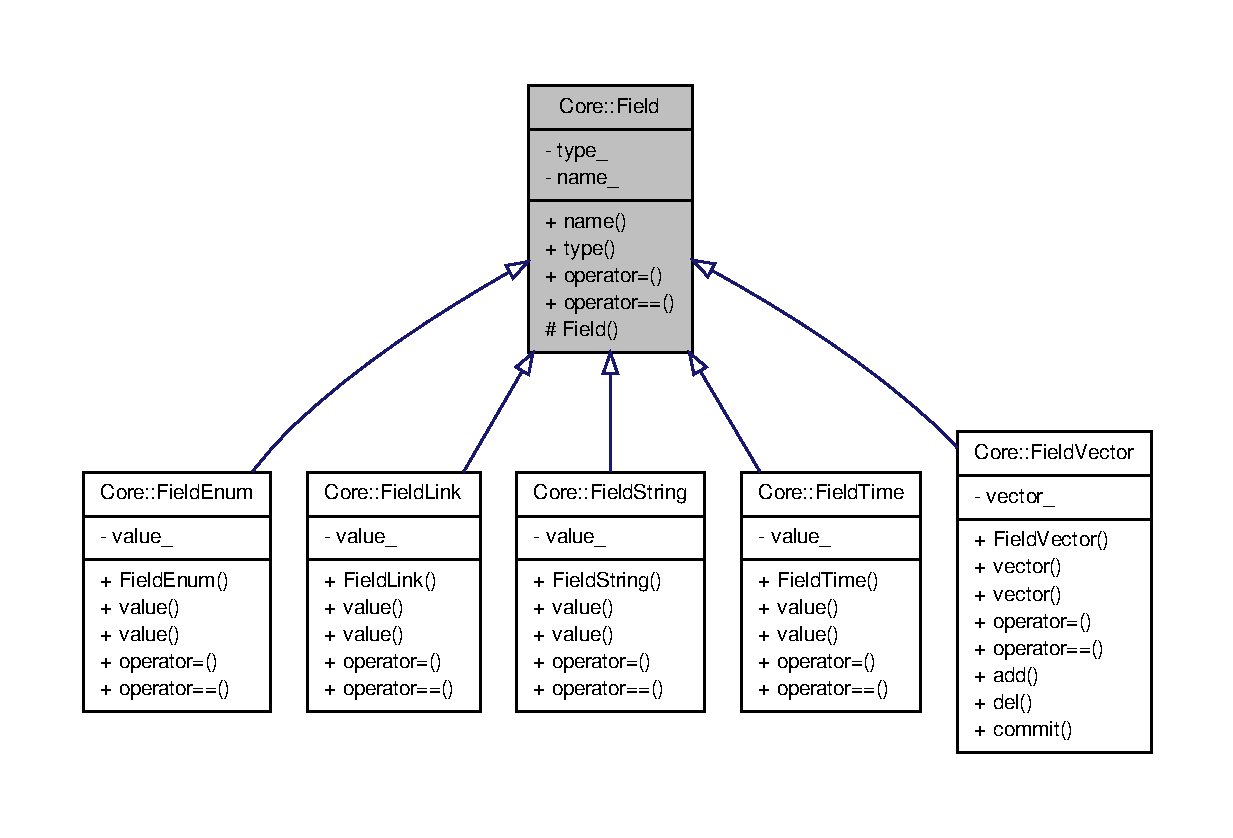
\includegraphics[width=400pt]{d1/dae/classCore_1_1Field__inherit__graph}
\end{center}
\end{figure}
\subsection*{Public Types}
\begin{DoxyCompactItemize}
\item 
enum \hyperlink{classCore_1_1Field_abd8b92d37ab4c79a2a15ec647c38cc9f}{Type} \{ \par
\hyperlink{classCore_1_1Field_abd8b92d37ab4c79a2a15ec647c38cc9fa286532cb5e3b52e8a222bed52a0ef230}{STRING}, 
\hyperlink{classCore_1_1Field_abd8b92d37ab4c79a2a15ec647c38cc9face3d1796b60e1f8a33a3ba5fc05e183d}{TIME}, 
\hyperlink{classCore_1_1Field_abd8b92d37ab4c79a2a15ec647c38cc9fa2b11372a326173242efdcb15bd28c567}{ENUM}, 
\hyperlink{classCore_1_1Field_abd8b92d37ab4c79a2a15ec647c38cc9fa9df866ca894748e77c04eda4bc9d32ee}{LINK}, 
\par
\hyperlink{classCore_1_1Field_abd8b92d37ab4c79a2a15ec647c38cc9fa57e09ea5a6d18aa8ebfae9c9bdcc9509}{VECTOR}
 \}
\begin{DoxyCompactList}\small\item\em Enumeration of possible field's types. \item\end{DoxyCompactList}\end{DoxyCompactItemize}
\subsection*{Public Member Functions}
\begin{DoxyCompactItemize}
\item 
const std::string \& \hyperlink{classCore_1_1Field_a3e49efbf0b184847c9fec35967268455}{name} () const   throw ()
\begin{DoxyCompactList}\small\item\em Get name of the field. \item\end{DoxyCompactList}\item 
const \hyperlink{classCore_1_1Field_abd8b92d37ab4c79a2a15ec647c38cc9f}{Type} \hyperlink{classCore_1_1Field_a92b8fa2a9a299655f8d4bd582023a7fa}{type} () const   throw ()
\begin{DoxyCompactList}\small\item\em Get type of the field. \item\end{DoxyCompactList}\item 
virtual const \hyperlink{classCore_1_1Field}{Field} \& \hyperlink{classCore_1_1Field_a3300f5867380b0e55bcd6c1918815e1f}{operator=} (const \hyperlink{classCore_1_1Field}{Field} \&field)=0  throw (std::bad\_\-cast)
\begin{DoxyCompactList}\small\item\em Assigment operator. \item\end{DoxyCompactList}\item 
virtual const bool \hyperlink{classCore_1_1Field_ae2db5ff861ee23a5d5cc43913544a4ab}{operator==} (const \hyperlink{classCore_1_1Field}{Field} \&field) const =0  throw (std::bad\_\-cast)
\begin{DoxyCompactList}\small\item\em Comparison operator. \item\end{DoxyCompactList}\end{DoxyCompactItemize}
\subsection*{Protected Member Functions}
\begin{DoxyCompactItemize}
\item 
\hyperlink{classCore_1_1Field_aeadb5d1caecc973dcaa12974443edba4}{Field} (const \hyperlink{classCore_1_1Field_abd8b92d37ab4c79a2a15ec647c38cc9f}{Type} type, const std::string \&name)  throw ()
\begin{DoxyCompactList}\small\item\em Constructor. \item\end{DoxyCompactList}\end{DoxyCompactItemize}


\subsection{Detailed Description}
Base class for fields of different types. \hyperlink{classCore_1_1Object}{Object} consist of field name, type and value. Value must be implemented in inherited classes. 

\subsection{Member Enumeration Documentation}
\hypertarget{classCore_1_1Field_abd8b92d37ab4c79a2a15ec647c38cc9f}{
\index{Core::Field@{Core::Field}!Type@{Type}}
\index{Type@{Type}!Core::Field@{Core::Field}}
\subsubsection[{Type}]{\setlength{\rightskip}{0pt plus 5cm}enum {\bf Core::Field::Type}}}
\label{dc/d16/classCore_1_1Field_abd8b92d37ab4c79a2a15ec647c38cc9f}


Enumeration of possible field's types. 

Used to check field type without typeid operator. \begin{Desc}
\item[Enumerator: ]\par
\begin{description}
\index{STRING@{STRING}!Core::Field@{Core::Field}}\index{Core::Field@{Core::Field}!STRING@{STRING}}\item[{\em 
\hypertarget{classCore_1_1Field_abd8b92d37ab4c79a2a15ec647c38cc9fa286532cb5e3b52e8a222bed52a0ef230}{
STRING}
\label{dc/d16/classCore_1_1Field_abd8b92d37ab4c79a2a15ec647c38cc9fa286532cb5e3b52e8a222bed52a0ef230}
}]\index{TIME@{TIME}!Core::Field@{Core::Field}}\index{Core::Field@{Core::Field}!TIME@{TIME}}\item[{\em 
\hypertarget{classCore_1_1Field_abd8b92d37ab4c79a2a15ec647c38cc9face3d1796b60e1f8a33a3ba5fc05e183d}{
TIME}
\label{dc/d16/classCore_1_1Field_abd8b92d37ab4c79a2a15ec647c38cc9face3d1796b60e1f8a33a3ba5fc05e183d}
}]\index{ENUM@{ENUM}!Core::Field@{Core::Field}}\index{Core::Field@{Core::Field}!ENUM@{ENUM}}\item[{\em 
\hypertarget{classCore_1_1Field_abd8b92d37ab4c79a2a15ec647c38cc9fa2b11372a326173242efdcb15bd28c567}{
ENUM}
\label{dc/d16/classCore_1_1Field_abd8b92d37ab4c79a2a15ec647c38cc9fa2b11372a326173242efdcb15bd28c567}
}]\index{LINK@{LINK}!Core::Field@{Core::Field}}\index{Core::Field@{Core::Field}!LINK@{LINK}}\item[{\em 
\hypertarget{classCore_1_1Field_abd8b92d37ab4c79a2a15ec647c38cc9fa9df866ca894748e77c04eda4bc9d32ee}{
LINK}
\label{dc/d16/classCore_1_1Field_abd8b92d37ab4c79a2a15ec647c38cc9fa9df866ca894748e77c04eda4bc9d32ee}
}]\index{VECTOR@{VECTOR}!Core::Field@{Core::Field}}\index{Core::Field@{Core::Field}!VECTOR@{VECTOR}}\item[{\em 
\hypertarget{classCore_1_1Field_abd8b92d37ab4c79a2a15ec647c38cc9fa57e09ea5a6d18aa8ebfae9c9bdcc9509}{
VECTOR}
\label{dc/d16/classCore_1_1Field_abd8b92d37ab4c79a2a15ec647c38cc9fa57e09ea5a6d18aa8ebfae9c9bdcc9509}
}]\end{description}
\end{Desc}



\subsection{Constructor \& Destructor Documentation}
\hypertarget{classCore_1_1Field_aeadb5d1caecc973dcaa12974443edba4}{
\index{Core::Field@{Core::Field}!Field@{Field}}
\index{Field@{Field}!Core::Field@{Core::Field}}
\subsubsection[{Field}]{\setlength{\rightskip}{0pt plus 5cm}Core::Field::Field (
\begin{DoxyParamCaption}
\item[{const {\bf Type}}]{type, }
\item[{const std::string \&}]{name}
\end{DoxyParamCaption}
)  throw ()\hspace{0.3cm}{\ttfamily  \mbox{[}inline, protected\mbox{]}}}}
\label{dc/d16/classCore_1_1Field_aeadb5d1caecc973dcaa12974443edba4}


Constructor. 

$<$ 
\begin{DoxyParams}[1]{Parameters}
\mbox{\tt in}  & {\em type} & Type of field. \\
\hline
\mbox{\tt in}  & {\em name} & Name of field. \\
\hline
\end{DoxyParams}


\subsection{Member Function Documentation}
\hypertarget{classCore_1_1Field_a3e49efbf0b184847c9fec35967268455}{
\index{Core::Field@{Core::Field}!name@{name}}
\index{name@{name}!Core::Field@{Core::Field}}
\subsubsection[{name}]{\setlength{\rightskip}{0pt plus 5cm}const std::string\& Core::Field::name (
\begin{DoxyParamCaption}
{}
\end{DoxyParamCaption}
) const  throw ()\hspace{0.3cm}{\ttfamily  \mbox{[}inline\mbox{]}}}}
\label{dc/d16/classCore_1_1Field_a3e49efbf0b184847c9fec35967268455}


Get name of the field. 

$<$ \begin{DoxyReturn}{Returns}
field's name. 
\end{DoxyReturn}


Here is the caller graph for this function:
\nopagebreak
\begin{figure}[H]
\begin{center}
\leavevmode
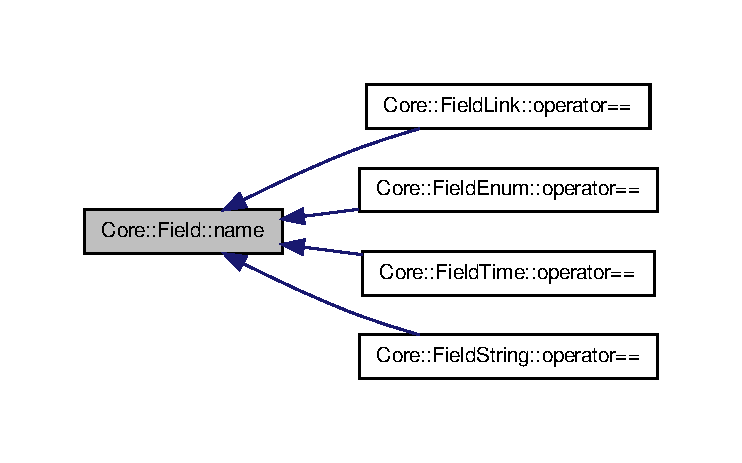
\includegraphics[width=356pt]{dc/d16/classCore_1_1Field_a3e49efbf0b184847c9fec35967268455_icgraph}
\end{center}
\end{figure}


\hypertarget{classCore_1_1Field_a3300f5867380b0e55bcd6c1918815e1f}{
\index{Core::Field@{Core::Field}!operator=@{operator=}}
\index{operator=@{operator=}!Core::Field@{Core::Field}}
\subsubsection[{operator=}]{\setlength{\rightskip}{0pt plus 5cm}virtual const {\bf Field}\& Core::Field::operator= (
\begin{DoxyParamCaption}
\item[{const {\bf Field} \&}]{field}
\end{DoxyParamCaption}
)  throw (std::bad\_\-cast)\hspace{0.3cm}{\ttfamily  \mbox{[}pure virtual\mbox{]}}}}
\label{dc/d16/classCore_1_1Field_a3300f5867380b0e55bcd6c1918815e1f}


Assigment operator. 


\begin{DoxyParams}[1]{Parameters}
\mbox{\tt in}  & {\em field} & \hyperlink{classCore_1_1Field}{Field} with value to assign. \\
\hline
\end{DoxyParams}
\begin{DoxyReturn}{Returns}
This field.
\end{DoxyReturn}
Assign this field's value to another fields value, if they have one type. 

Implemented in \hyperlink{classCore_1_1FieldString_a78a8bc98252c1be096848c5cdebb2868}{Core::FieldString}, \hyperlink{classCore_1_1FieldTime_ab0b9e7fe5ee619d3d584dfd3a9be5015}{Core::FieldTime}, \hyperlink{classCore_1_1FieldEnum_ab0e6e56ee028b5ba08e47edb14d76be1}{Core::FieldEnum}, \hyperlink{classCore_1_1FieldLink_a3690c623f44e77dee5a70dd13e713a76}{Core::FieldLink}, and \hyperlink{classCore_1_1FieldVector_a8482c272e2bc4e5b09194b903bead7f7}{Core::FieldVector}.

\hypertarget{classCore_1_1Field_ae2db5ff861ee23a5d5cc43913544a4ab}{
\index{Core::Field@{Core::Field}!operator==@{operator==}}
\index{operator==@{operator==}!Core::Field@{Core::Field}}
\subsubsection[{operator==}]{\setlength{\rightskip}{0pt plus 5cm}virtual const bool Core::Field::operator== (
\begin{DoxyParamCaption}
\item[{const {\bf Field} \&}]{field}
\end{DoxyParamCaption}
) const  throw (std::bad\_\-cast)\hspace{0.3cm}{\ttfamily  \mbox{[}pure virtual\mbox{]}}}}
\label{dc/d16/classCore_1_1Field_ae2db5ff861ee23a5d5cc43913544a4ab}


Comparison operator. 


\begin{DoxyParams}[1]{Parameters}
\mbox{\tt in}  & {\em field} & \hyperlink{classCore_1_1Field}{Field} with value to compare. \\
\hline
\end{DoxyParams}
\begin{DoxyReturn}{Returns}
result of comparison.
\end{DoxyReturn}
Compare values of two fields, if they have one type. 

Implemented in \hyperlink{classCore_1_1FieldString_adacfe0012314f6840b2657d63ffe8c49}{Core::FieldString}, \hyperlink{classCore_1_1FieldTime_aa48c2e4d7c6ad13794f66f3e59849843}{Core::FieldTime}, \hyperlink{classCore_1_1FieldEnum_a49097e37b11fb74375e89f365aee9c31}{Core::FieldEnum}, \hyperlink{classCore_1_1FieldLink_abffb8e3af41aabd4d82671e6e6cefb14}{Core::FieldLink}, and \hyperlink{classCore_1_1FieldVector_a79df85b6378b5ce608ca579bd3e23027}{Core::FieldVector}.

\hypertarget{classCore_1_1Field_a92b8fa2a9a299655f8d4bd582023a7fa}{
\index{Core::Field@{Core::Field}!type@{type}}
\index{type@{type}!Core::Field@{Core::Field}}
\subsubsection[{type}]{\setlength{\rightskip}{0pt plus 5cm}const {\bf Type} Core::Field::type (
\begin{DoxyParamCaption}
{}
\end{DoxyParamCaption}
) const  throw ()\hspace{0.3cm}{\ttfamily  \mbox{[}inline\mbox{]}}}}
\label{dc/d16/classCore_1_1Field_a92b8fa2a9a299655f8d4bd582023a7fa}


Get type of the field. 

$<$ \begin{DoxyReturn}{Returns}
field's type. 
\end{DoxyReturn}


The documentation for this class was generated from the following file:\begin{DoxyCompactItemize}
\item 
src/include/\hyperlink{field_8h}{field.h}\end{DoxyCompactItemize}

\hypertarget{classCore_1_1FieldEnum}{
\section{Core::FieldEnum Class Reference}
\label{d3/db7/classCore_1_1FieldEnum}\index{Core::FieldEnum@{Core::FieldEnum}}
}


\hyperlink{classCore_1_1Field}{Field} of std::string type but used for enumeration.  




{\ttfamily \#include $<$field.h$>$}



Inheritance diagram for Core::FieldEnum:
\nopagebreak
\begin{figure}[H]
\begin{center}
\leavevmode
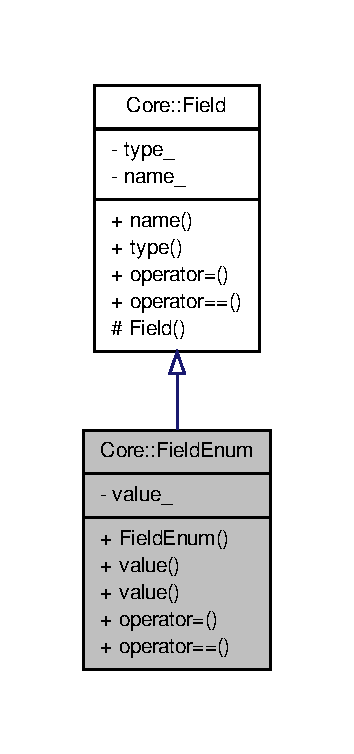
\includegraphics[width=170pt]{d1/d93/classCore_1_1FieldEnum__inherit__graph}
\end{center}
\end{figure}


Collaboration diagram for Core::FieldEnum:
\nopagebreak
\begin{figure}[H]
\begin{center}
\leavevmode
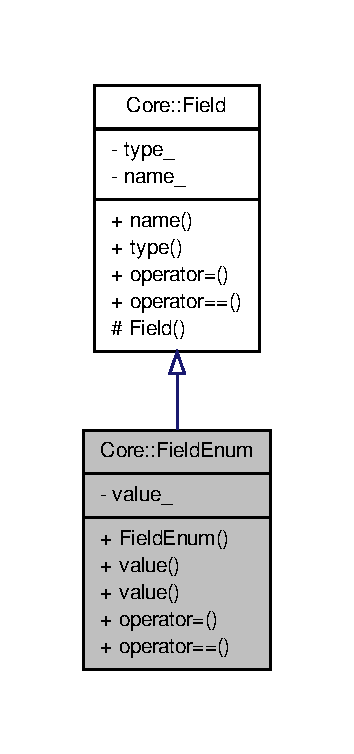
\includegraphics[width=170pt]{d6/db1/classCore_1_1FieldEnum__coll__graph}
\end{center}
\end{figure}
\subsection*{Public Member Functions}
\begin{DoxyCompactItemize}
\item 
\hyperlink{classCore_1_1FieldEnum_acd36404569789f33d1fbbbc7580dee98}{FieldEnum} (const std::string \&name, const std::string \&value)  throw ()
\begin{DoxyCompactList}\small\item\em Constructor. \item\end{DoxyCompactList}\item 
const std::string \& \hyperlink{classCore_1_1FieldEnum_a50d449354fbca83fc51c2feb1d06bb9e}{value} (const std::string \&value)  throw (std::bad\_\-cast)
\item 
const std::string \& \hyperlink{classCore_1_1FieldEnum_af10b8aa54cc84acda18cbf85614e26f2}{value} () const   throw ()
\item 
virtual const \hyperlink{classCore_1_1Field}{Field} \& \hyperlink{classCore_1_1FieldEnum_ab0e6e56ee028b5ba08e47edb14d76be1}{operator=} (const \hyperlink{classCore_1_1Field}{Field} \&field)  throw (std::bad\_\-cast)
\item 
virtual const bool \hyperlink{classCore_1_1FieldEnum_a49097e37b11fb74375e89f365aee9c31}{operator==} (const \hyperlink{classCore_1_1Field}{Field} \&field) const   throw (std::bad\_\-cast)
\end{DoxyCompactItemize}


\subsection{Detailed Description}
\hyperlink{classCore_1_1Field}{Field} of std::string type but used for enumeration. Simple class contains name and std::string value. 

It is fully equal to \hyperlink{classCore_1_1FieldString}{Core::FieldString}, but for strong type identification it is copied instead of using typedef. It has done to deny next ways of code:


\begin{DoxyCode}
 Core::FieldString string("some_field");
 Core::FieldEnum enum("some_enum", "some_value");
 string = enum;
 //---- or -------
 string = dynamic_cast<Core::FieldString>(enum);
\end{DoxyCode}


But next way is correct:


\begin{DoxyCode}
 Core::FieldString string("some_field");
 Core::FieldEnum enum("some_enum", "some_value");
 string.value(enum.value());
\end{DoxyCode}


Value of this class can not be empty. This class different from \hyperlink{classCore_1_1FieldString}{Core::FieldString} by this. 

\subsection{Constructor \& Destructor Documentation}
\hypertarget{classCore_1_1FieldEnum_acd36404569789f33d1fbbbc7580dee98}{
\index{Core::FieldEnum@{Core::FieldEnum}!FieldEnum@{FieldEnum}}
\index{FieldEnum@{FieldEnum}!Core::FieldEnum@{Core::FieldEnum}}
\subsubsection[{FieldEnum}]{\setlength{\rightskip}{0pt plus 5cm}Core::FieldEnum::FieldEnum (
\begin{DoxyParamCaption}
\item[{const std::string \&}]{name, }
\item[{const std::string \&}]{value}
\end{DoxyParamCaption}
)  throw ()\hspace{0.3cm}{\ttfamily  \mbox{[}inline\mbox{]}}}}
\label{d3/db7/classCore_1_1FieldEnum_acd36404569789f33d1fbbbc7580dee98}


Constructor. 

$<$ 
\begin{DoxyParams}[1]{Parameters}
\mbox{\tt in}  & {\em name} & Name of the field. \\
\hline
\mbox{\tt in}  & {\em value} & Value of the field. \\
\hline
\end{DoxyParams}


\subsection{Member Function Documentation}
\hypertarget{classCore_1_1FieldEnum_ab0e6e56ee028b5ba08e47edb14d76be1}{
\index{Core::FieldEnum@{Core::FieldEnum}!operator=@{operator=}}
\index{operator=@{operator=}!Core::FieldEnum@{Core::FieldEnum}}
\subsubsection[{operator=}]{\setlength{\rightskip}{0pt plus 5cm}virtual const {\bf Field}\& Core::FieldEnum::operator= (
\begin{DoxyParamCaption}
\item[{const {\bf Field} \&}]{field}
\end{DoxyParamCaption}
)  throw (std::bad\_\-cast)\hspace{0.3cm}{\ttfamily  \mbox{[}inline, virtual\mbox{]}}}}
\label{d3/db7/classCore_1_1FieldEnum_ab0e6e56ee028b5ba08e47edb14d76be1}
$<$ $<$ Assigment operator. 


\begin{DoxyParams}[1]{Parameters}
\mbox{\tt in}  & {\em field} & \hyperlink{classCore_1_1Field}{Field} with value to assign. \\
\hline
\end{DoxyParams}
\begin{DoxyReturn}{Returns}
This field.
\end{DoxyReturn}
Assign this field's value to another fields value, if they have one type.  Implementation for std::string type.  

Implements \hyperlink{classCore_1_1Field_a3300f5867380b0e55bcd6c1918815e1f}{Core::Field}.



Here is the call graph for this function:
\nopagebreak
\begin{figure}[H]
\begin{center}
\leavevmode
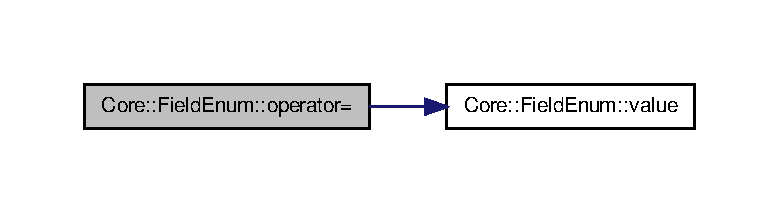
\includegraphics[width=374pt]{d3/db7/classCore_1_1FieldEnum_ab0e6e56ee028b5ba08e47edb14d76be1_cgraph}
\end{center}
\end{figure}


\hypertarget{classCore_1_1FieldEnum_a49097e37b11fb74375e89f365aee9c31}{
\index{Core::FieldEnum@{Core::FieldEnum}!operator==@{operator==}}
\index{operator==@{operator==}!Core::FieldEnum@{Core::FieldEnum}}
\subsubsection[{operator==}]{\setlength{\rightskip}{0pt plus 5cm}virtual const bool Core::FieldEnum::operator== (
\begin{DoxyParamCaption}
\item[{const {\bf Field} \&}]{field}
\end{DoxyParamCaption}
) const  throw (std::bad\_\-cast)\hspace{0.3cm}{\ttfamily  \mbox{[}inline, virtual\mbox{]}}}}
\label{d3/db7/classCore_1_1FieldEnum_a49097e37b11fb74375e89f365aee9c31}
$<$ $<$ Comparison operator. 


\begin{DoxyParams}[1]{Parameters}
\mbox{\tt in}  & {\em field} & \hyperlink{classCore_1_1Field}{Field} with value to compare. \\
\hline
\end{DoxyParams}
\begin{DoxyReturn}{Returns}
result of comparison.
\end{DoxyReturn}
Compare values of two fields, if they have one type.  Implementation for std::string type.  

Implements \hyperlink{classCore_1_1Field_ae2db5ff861ee23a5d5cc43913544a4ab}{Core::Field}.



Here is the call graph for this function:
\nopagebreak
\begin{figure}[H]
\begin{center}
\leavevmode
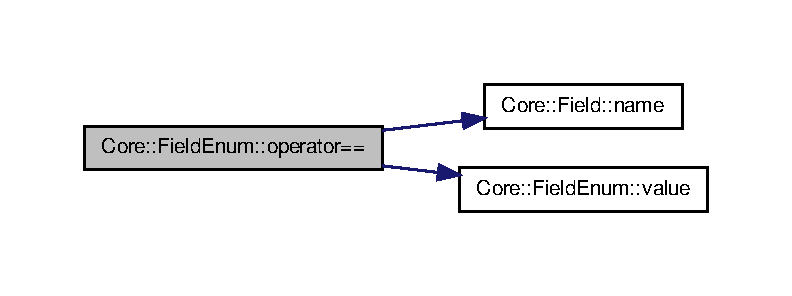
\includegraphics[width=380pt]{d3/db7/classCore_1_1FieldEnum_a49097e37b11fb74375e89f365aee9c31_cgraph}
\end{center}
\end{figure}


\hypertarget{classCore_1_1FieldEnum_a50d449354fbca83fc51c2feb1d06bb9e}{
\index{Core::FieldEnum@{Core::FieldEnum}!value@{value}}
\index{value@{value}!Core::FieldEnum@{Core::FieldEnum}}
\subsubsection[{value}]{\setlength{\rightskip}{0pt plus 5cm}const std::string\& Core::FieldEnum::value (
\begin{DoxyParamCaption}
\item[{const std::string \&}]{value}
\end{DoxyParamCaption}
)  throw (std::bad\_\-cast)\hspace{0.3cm}{\ttfamily  \mbox{[}inline\mbox{]}}}}
\label{d3/db7/classCore_1_1FieldEnum_a50d449354fbca83fc51c2feb1d06bb9e}
$<$ Change value. 

$<$ 
\begin{DoxyParams}[1]{Parameters}
\mbox{\tt in}  & {\em New} & value of the field. \\
\hline
\end{DoxyParams}
\begin{DoxyReturn}{Returns}
Value of the field AFTER assigment. 
\end{DoxyReturn}
 This method throws {\ttfamily std::bad\_\-cast} exception if {\itshape value\/} is empty. 

Here is the call graph for this function:
\nopagebreak
\begin{figure}[H]
\begin{center}
\leavevmode
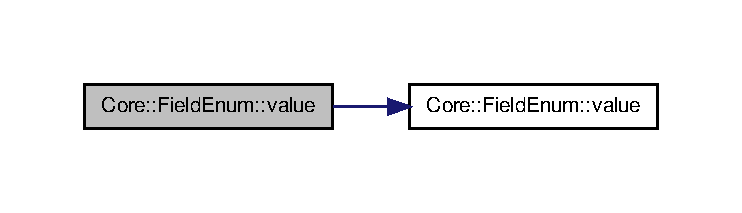
\includegraphics[width=356pt]{d3/db7/classCore_1_1FieldEnum_a50d449354fbca83fc51c2feb1d06bb9e_cgraph}
\end{center}
\end{figure}


\hypertarget{classCore_1_1FieldEnum_af10b8aa54cc84acda18cbf85614e26f2}{
\index{Core::FieldEnum@{Core::FieldEnum}!value@{value}}
\index{value@{value}!Core::FieldEnum@{Core::FieldEnum}}
\subsubsection[{value}]{\setlength{\rightskip}{0pt plus 5cm}const std::string\& Core::FieldEnum::value (
\begin{DoxyParamCaption}
{}
\end{DoxyParamCaption}
) const  throw ()\hspace{0.3cm}{\ttfamily  \mbox{[}inline\mbox{]}}}}
\label{d3/db7/classCore_1_1FieldEnum_af10b8aa54cc84acda18cbf85614e26f2}
$<$ Change value. 

$<$ 
\begin{DoxyParams}[1]{Parameters}
\mbox{\tt in}  & {\em New} & value of the field. \\
\hline
\end{DoxyParams}
\begin{DoxyReturn}{Returns}
Value of the field AFTER assigment. 
\end{DoxyReturn}
 

Here is the caller graph for this function:
\nopagebreak
\begin{figure}[H]
\begin{center}
\leavevmode
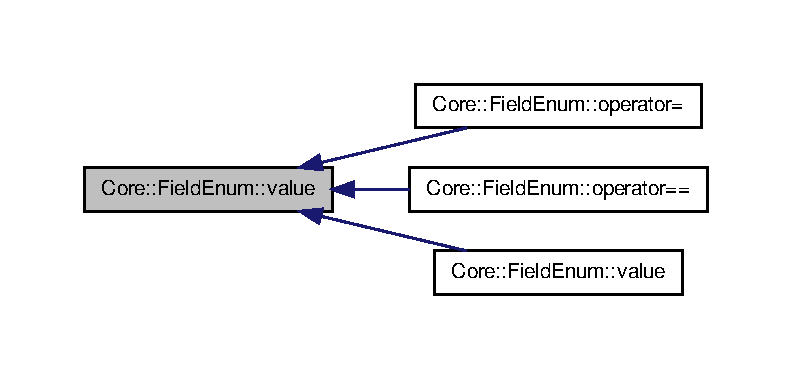
\includegraphics[width=380pt]{d3/db7/classCore_1_1FieldEnum_af10b8aa54cc84acda18cbf85614e26f2_icgraph}
\end{center}
\end{figure}




The documentation for this class was generated from the following file:\begin{DoxyCompactItemize}
\item 
src/include/\hyperlink{field_8h}{field.h}\end{DoxyCompactItemize}

\hypertarget{classCore_1_1FieldLink}{
\section{Core::FieldLink Class Reference}
\label{d9/d23/classCore_1_1FieldLink}\index{Core::FieldLink@{Core::FieldLink}}
}


Link of two objects.  




{\ttfamily \#include $<$field.h$>$}



Inheritance diagram for Core::FieldLink:
\nopagebreak
\begin{figure}[H]
\begin{center}
\leavevmode
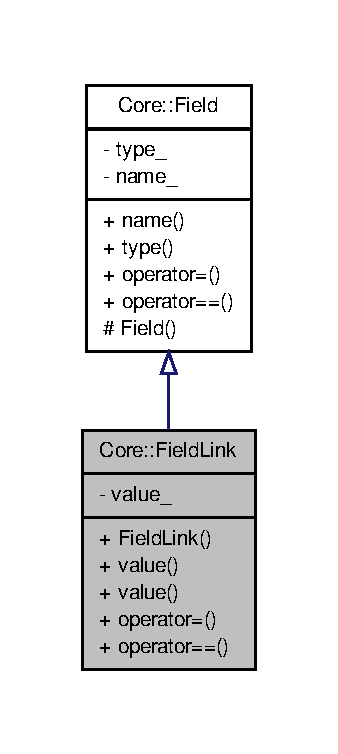
\includegraphics[width=162pt]{de/db8/classCore_1_1FieldLink__inherit__graph}
\end{center}
\end{figure}


Collaboration diagram for Core::FieldLink:
\nopagebreak
\begin{figure}[H]
\begin{center}
\leavevmode
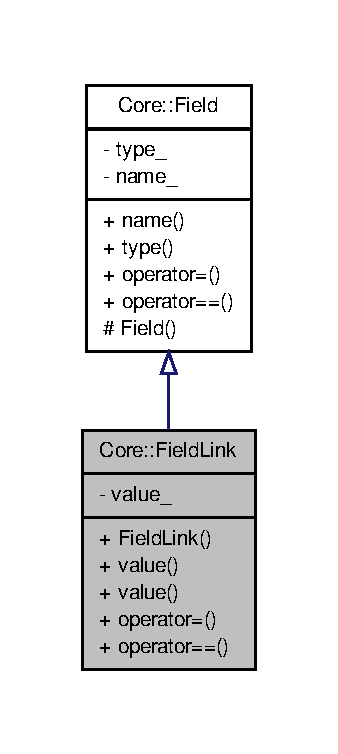
\includegraphics[width=162pt]{dd/dad/classCore_1_1FieldLink__coll__graph}
\end{center}
\end{figure}
\subsection*{Public Member Functions}
\begin{DoxyCompactItemize}
\item 
\hyperlink{classCore_1_1FieldLink_a54d7afaa568554c610dd2d404ee73a4f}{FieldLink} (const std::string \&name, const std::pair$<$ \hyperlink{classCore_1_1Object}{Object} $\ast$, bool $>$ \&value)  throw ()
\begin{DoxyCompactList}\small\item\em Constructor. \item\end{DoxyCompactList}\item 
std::pair$<$ \hyperlink{classCore_1_1Object}{Object} $\ast$, bool $>$ \hyperlink{classCore_1_1FieldLink_a0b43b80b0e6f7aeb08b763051bde0b80}{value} (const std::pair$<$ \hyperlink{classCore_1_1Object}{Object} $\ast$, bool $>$ \&value)  throw ()
\item 
std::pair$<$ \hyperlink{classCore_1_1Object}{Object} $\ast$, bool $>$ \hyperlink{classCore_1_1FieldLink_add648c4cde8a23233384ca213874cf0d}{value} () const   throw ()
\item 
virtual const \hyperlink{classCore_1_1Field}{Field} \& \hyperlink{classCore_1_1FieldLink_a3690c623f44e77dee5a70dd13e713a76}{operator=} (const \hyperlink{classCore_1_1Field}{Field} \&field)  throw (std::bad\_\-cast)
\item 
virtual const bool \hyperlink{classCore_1_1FieldLink_abffb8e3af41aabd4d82671e6e6cefb14}{operator==} (const \hyperlink{classCore_1_1Field}{Field} \&field) const   throw (std::bad\_\-cast)
\end{DoxyCompactItemize}


\subsection{Detailed Description}
Link of two objects. Class, contains name, pointer to object and flag (link/unlink). Use to change vectors of objects. 

\subsection{Constructor \& Destructor Documentation}
\hypertarget{classCore_1_1FieldLink_a54d7afaa568554c610dd2d404ee73a4f}{
\index{Core::FieldLink@{Core::FieldLink}!FieldLink@{FieldLink}}
\index{FieldLink@{FieldLink}!Core::FieldLink@{Core::FieldLink}}
\subsubsection[{FieldLink}]{\setlength{\rightskip}{0pt plus 5cm}Core::FieldLink::FieldLink (
\begin{DoxyParamCaption}
\item[{const std::string \&}]{name, }
\item[{const std::pair$<$ {\bf Object} $\ast$, bool $>$ \&}]{value}
\end{DoxyParamCaption}
)  throw ()\hspace{0.3cm}{\ttfamily  \mbox{[}inline\mbox{]}}}}
\label{d9/d23/classCore_1_1FieldLink_a54d7afaa568554c610dd2d404ee73a4f}


Constructor. 

$<$ 
\begin{DoxyParams}[1]{Parameters}
\mbox{\tt in}  & {\em name} & Name of the field. \\
\hline
\mbox{\tt in}  & {\em value} & \hyperlink{classCore_1_1Object}{Object} and state of link. \\
\hline
\end{DoxyParams}


\subsection{Member Function Documentation}
\hypertarget{classCore_1_1FieldLink_a3690c623f44e77dee5a70dd13e713a76}{
\index{Core::FieldLink@{Core::FieldLink}!operator=@{operator=}}
\index{operator=@{operator=}!Core::FieldLink@{Core::FieldLink}}
\subsubsection[{operator=}]{\setlength{\rightskip}{0pt plus 5cm}virtual const {\bf Field}\& Core::FieldLink::operator= (
\begin{DoxyParamCaption}
\item[{const {\bf Field} \&}]{field}
\end{DoxyParamCaption}
)  throw (std::bad\_\-cast)\hspace{0.3cm}{\ttfamily  \mbox{[}inline, virtual\mbox{]}}}}
\label{d9/d23/classCore_1_1FieldLink_a3690c623f44e77dee5a70dd13e713a76}
$<$ Assigment operator. 


\begin{DoxyParams}[1]{Parameters}
\mbox{\tt in}  & {\em field} & \hyperlink{classCore_1_1Field}{Field} with value to assign. \\
\hline
\end{DoxyParams}
\begin{DoxyReturn}{Returns}
This field.
\end{DoxyReturn}
Assign this field's value to another fields value, if they have one type.  Implementation for Link type. 

Implements \hyperlink{classCore_1_1Field_a3300f5867380b0e55bcd6c1918815e1f}{Core::Field}.



Here is the call graph for this function:
\nopagebreak
\begin{figure}[H]
\begin{center}
\leavevmode
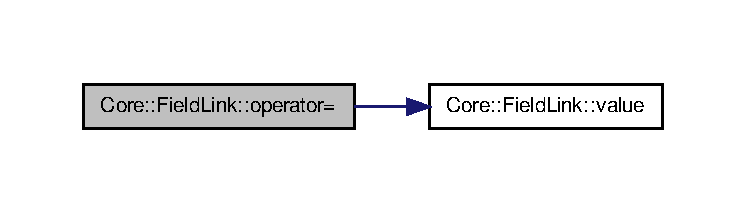
\includegraphics[width=358pt]{d9/d23/classCore_1_1FieldLink_a3690c623f44e77dee5a70dd13e713a76_cgraph}
\end{center}
\end{figure}


\hypertarget{classCore_1_1FieldLink_abffb8e3af41aabd4d82671e6e6cefb14}{
\index{Core::FieldLink@{Core::FieldLink}!operator==@{operator==}}
\index{operator==@{operator==}!Core::FieldLink@{Core::FieldLink}}
\subsubsection[{operator==}]{\setlength{\rightskip}{0pt plus 5cm}virtual const bool Core::FieldLink::operator== (
\begin{DoxyParamCaption}
\item[{const {\bf Field} \&}]{field}
\end{DoxyParamCaption}
) const  throw (std::bad\_\-cast)\hspace{0.3cm}{\ttfamily  \mbox{[}inline, virtual\mbox{]}}}}
\label{d9/d23/classCore_1_1FieldLink_abffb8e3af41aabd4d82671e6e6cefb14}
$<$ Comparison operator. 


\begin{DoxyParams}[1]{Parameters}
\mbox{\tt in}  & {\em field} & \hyperlink{classCore_1_1Field}{Field} with value to compare. \\
\hline
\end{DoxyParams}
\begin{DoxyReturn}{Returns}
result of comparison.
\end{DoxyReturn}
Compare values of two fields, if they have one type.  Implementation for Link type. 

Implements \hyperlink{classCore_1_1Field_ae2db5ff861ee23a5d5cc43913544a4ab}{Core::Field}.



Here is the call graph for this function:
\nopagebreak
\begin{figure}[H]
\begin{center}
\leavevmode
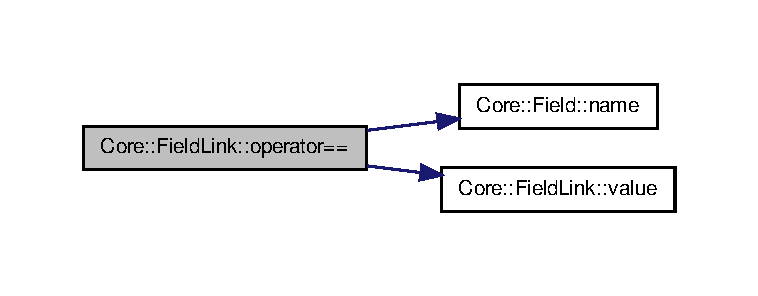
\includegraphics[width=364pt]{d9/d23/classCore_1_1FieldLink_abffb8e3af41aabd4d82671e6e6cefb14_cgraph}
\end{center}
\end{figure}


\hypertarget{classCore_1_1FieldLink_a0b43b80b0e6f7aeb08b763051bde0b80}{
\index{Core::FieldLink@{Core::FieldLink}!value@{value}}
\index{value@{value}!Core::FieldLink@{Core::FieldLink}}
\subsubsection[{value}]{\setlength{\rightskip}{0pt plus 5cm}std::pair$<${\bf Object} $\ast$, bool$>$ Core::FieldLink::value (
\begin{DoxyParamCaption}
\item[{const std::pair$<$ {\bf Object} $\ast$, bool $>$ \&}]{value}
\end{DoxyParamCaption}
)  throw ()\hspace{0.3cm}{\ttfamily  \mbox{[}inline\mbox{]}}}}
\label{d9/d23/classCore_1_1FieldLink_a0b43b80b0e6f7aeb08b763051bde0b80}
$<$ Change value. 

$<$ 
\begin{DoxyParams}[1]{Parameters}
\mbox{\tt in}  & {\em New} & value of the field. \\
\hline
\end{DoxyParams}
\begin{DoxyReturn}{Returns}
Value of the field AFTER assigment. 
\end{DoxyReturn}
 

Here is the call graph for this function:
\nopagebreak
\begin{figure}[H]
\begin{center}
\leavevmode
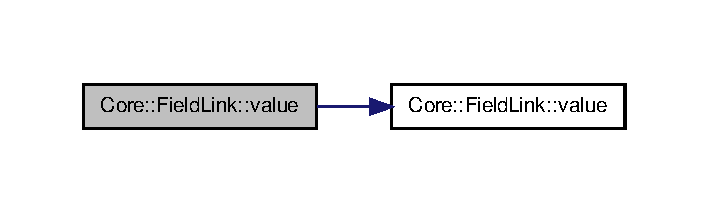
\includegraphics[width=340pt]{d9/d23/classCore_1_1FieldLink_a0b43b80b0e6f7aeb08b763051bde0b80_cgraph}
\end{center}
\end{figure}




Here is the caller graph for this function:
\nopagebreak
\begin{figure}[H]
\begin{center}
\leavevmode
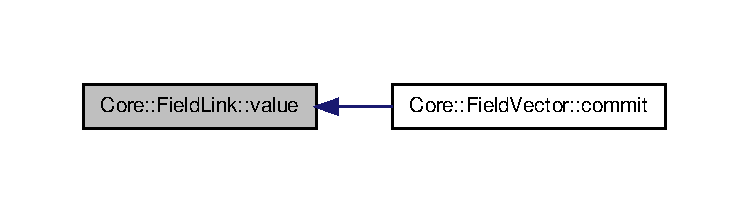
\includegraphics[width=360pt]{d9/d23/classCore_1_1FieldLink_a0b43b80b0e6f7aeb08b763051bde0b80_icgraph}
\end{center}
\end{figure}


\hypertarget{classCore_1_1FieldLink_add648c4cde8a23233384ca213874cf0d}{
\index{Core::FieldLink@{Core::FieldLink}!value@{value}}
\index{value@{value}!Core::FieldLink@{Core::FieldLink}}
\subsubsection[{value}]{\setlength{\rightskip}{0pt plus 5cm}std::pair$<${\bf Object} $\ast$, bool$>$ Core::FieldLink::value (
\begin{DoxyParamCaption}
{}
\end{DoxyParamCaption}
) const  throw ()\hspace{0.3cm}{\ttfamily  \mbox{[}inline\mbox{]}}}}
\label{d9/d23/classCore_1_1FieldLink_add648c4cde8a23233384ca213874cf0d}
$<$ Change value. 

$<$ 
\begin{DoxyParams}[1]{Parameters}
\mbox{\tt in}  & {\em New} & value of the field. \\
\hline
\end{DoxyParams}
\begin{DoxyReturn}{Returns}
Value of the field AFTER assigment. 
\end{DoxyReturn}
 

Here is the caller graph for this function:
\nopagebreak
\begin{figure}[H]
\begin{center}
\leavevmode
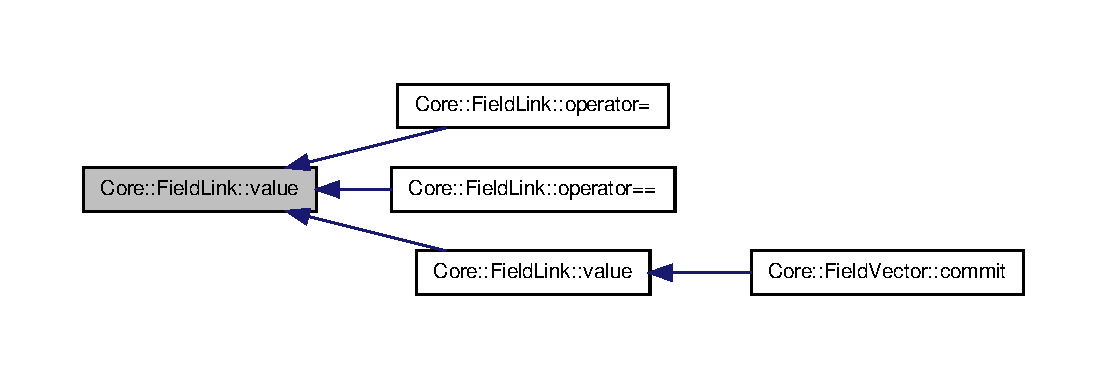
\includegraphics[width=400pt]{d9/d23/classCore_1_1FieldLink_add648c4cde8a23233384ca213874cf0d_icgraph}
\end{center}
\end{figure}




The documentation for this class was generated from the following file:\begin{DoxyCompactItemize}
\item 
src/include/\hyperlink{field_8h}{field.h}\end{DoxyCompactItemize}

\hypertarget{classCore_1_1FieldString}{
\section{Core::FieldString Class Reference}
\label{dd/d02/classCore_1_1FieldString}\index{Core::FieldString@{Core::FieldString}}
}


\hyperlink{classCore_1_1Field}{Field} of string type.  




{\ttfamily \#include $<$field.h$>$}



Inheritance diagram for Core::FieldString:
\nopagebreak
\begin{figure}[H]
\begin{center}
\leavevmode
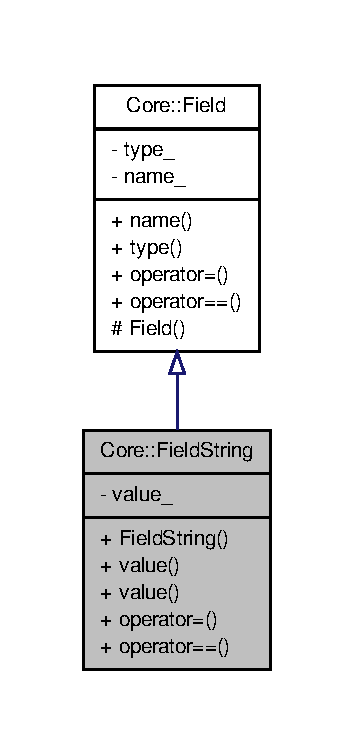
\includegraphics[width=170pt]{d6/d1c/classCore_1_1FieldString__inherit__graph}
\end{center}
\end{figure}


Collaboration diagram for Core::FieldString:
\nopagebreak
\begin{figure}[H]
\begin{center}
\leavevmode
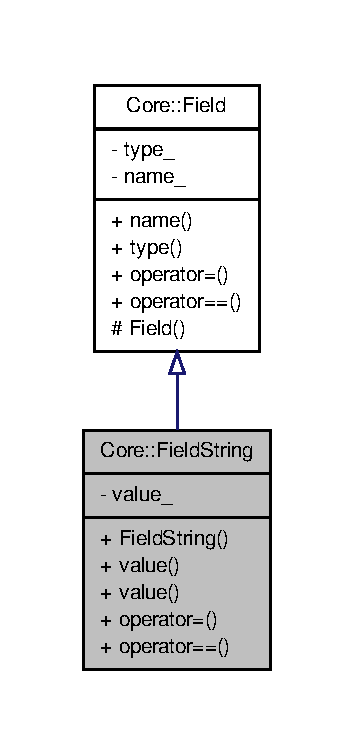
\includegraphics[width=170pt]{d3/df7/classCore_1_1FieldString__coll__graph}
\end{center}
\end{figure}
\subsection*{Public Member Functions}
\begin{DoxyCompactItemize}
\item 
\hyperlink{classCore_1_1FieldString_aeea00d447ccc028124716bef705b9359}{FieldString} (const std::string \&name, const std::string \&value=\char`\"{}\char`\"{})  throw ()
\begin{DoxyCompactList}\small\item\em Constructor. \item\end{DoxyCompactList}\item 
const std::string \& \hyperlink{classCore_1_1FieldString_a1cf5a18e64379806684e0bb110a002d1}{value} (const std::string \&value)  throw ()
\begin{DoxyCompactList}\small\item\em Change value. \item\end{DoxyCompactList}\item 
const std::string \& \hyperlink{classCore_1_1FieldString_a31f2a21becad6221f033daaf8aa161d7}{value} () const   throw ()
\begin{DoxyCompactList}\small\item\em Get value. \item\end{DoxyCompactList}\item 
virtual \hyperlink{classCore_1_1Field}{Field} \& \hyperlink{classCore_1_1FieldString_a78a8bc98252c1be096848c5cdebb2868}{operator=} (const \hyperlink{classCore_1_1Field}{Field} \&field)  throw (std::bad\_\-cast)
\item 
virtual const bool \hyperlink{classCore_1_1FieldString_adacfe0012314f6840b2657d63ffe8c49}{operator==} (const \hyperlink{classCore_1_1Field}{Field} \&field) const   throw (std::bad\_\-cast)
\end{DoxyCompactItemize}


\subsection{Detailed Description}
\hyperlink{classCore_1_1Field}{Field} of string type. Simple class contains name and std::string value. 

\subsection{Constructor \& Destructor Documentation}
\hypertarget{classCore_1_1FieldString_aeea00d447ccc028124716bef705b9359}{
\index{Core::FieldString@{Core::FieldString}!FieldString@{FieldString}}
\index{FieldString@{FieldString}!Core::FieldString@{Core::FieldString}}
\subsubsection[{FieldString}]{\setlength{\rightskip}{0pt plus 5cm}Core::FieldString::FieldString (
\begin{DoxyParamCaption}
\item[{const std::string \&}]{name, }
\item[{const std::string \&}]{value = {\ttfamily \char`\"{}\char`\"{}}}
\end{DoxyParamCaption}
)  throw ()\hspace{0.3cm}{\ttfamily  \mbox{[}inline\mbox{]}}}}
\label{dd/d02/classCore_1_1FieldString_aeea00d447ccc028124716bef705b9359}


Constructor. 

$<$ 
\begin{DoxyParams}[1]{Parameters}
\mbox{\tt in}  & {\em name} & Name of the field. \\
\hline
\mbox{\tt in}  & {\em value} & Value of the field. Empty by default. \\
\hline
\end{DoxyParams}


\subsection{Member Function Documentation}
\hypertarget{classCore_1_1FieldString_a78a8bc98252c1be096848c5cdebb2868}{
\index{Core::FieldString@{Core::FieldString}!operator=@{operator=}}
\index{operator=@{operator=}!Core::FieldString@{Core::FieldString}}
\subsubsection[{operator=}]{\setlength{\rightskip}{0pt plus 5cm}virtual {\bf Field}\& Core::FieldString::operator= (
\begin{DoxyParamCaption}
\item[{const {\bf Field} \&}]{field}
\end{DoxyParamCaption}
)  throw (std::bad\_\-cast)\hspace{0.3cm}{\ttfamily  \mbox{[}inline, virtual\mbox{]}}}}
\label{dd/d02/classCore_1_1FieldString_a78a8bc98252c1be096848c5cdebb2868}
$<$ Assigment operator. 


\begin{DoxyParams}[1]{Parameters}
\mbox{\tt in}  & {\em field} & \hyperlink{classCore_1_1Field}{Field} with value to assign. \\
\hline
\end{DoxyParams}
\begin{DoxyReturn}{Returns}
This field.
\end{DoxyReturn}
Assign this field's value to another fields value, if they have one type.  Implementation for std::string type. 

Implements \hyperlink{classCore_1_1Field_a3300f5867380b0e55bcd6c1918815e1f}{Core::Field}.



Here is the call graph for this function:
\nopagebreak
\begin{figure}[H]
\begin{center}
\leavevmode
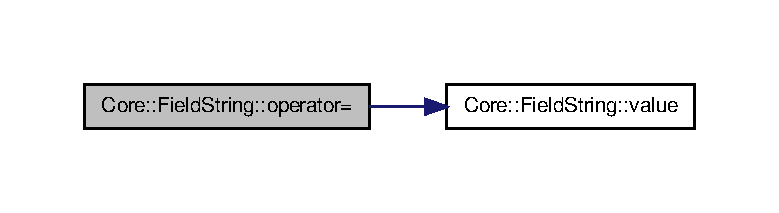
\includegraphics[width=374pt]{dd/d02/classCore_1_1FieldString_a78a8bc98252c1be096848c5cdebb2868_cgraph}
\end{center}
\end{figure}


\hypertarget{classCore_1_1FieldString_adacfe0012314f6840b2657d63ffe8c49}{
\index{Core::FieldString@{Core::FieldString}!operator==@{operator==}}
\index{operator==@{operator==}!Core::FieldString@{Core::FieldString}}
\subsubsection[{operator==}]{\setlength{\rightskip}{0pt plus 5cm}virtual const bool Core::FieldString::operator== (
\begin{DoxyParamCaption}
\item[{const {\bf Field} \&}]{field}
\end{DoxyParamCaption}
) const  throw (std::bad\_\-cast)\hspace{0.3cm}{\ttfamily  \mbox{[}inline, virtual\mbox{]}}}}
\label{dd/d02/classCore_1_1FieldString_adacfe0012314f6840b2657d63ffe8c49}
$<$ Comparison operator. 


\begin{DoxyParams}[1]{Parameters}
\mbox{\tt in}  & {\em field} & \hyperlink{classCore_1_1Field}{Field} with value to compare. \\
\hline
\end{DoxyParams}
\begin{DoxyReturn}{Returns}
result of comparison.
\end{DoxyReturn}
Compare values of two fields, if they have one type.  Implementation for std::string type. 

Implements \hyperlink{classCore_1_1Field_ae2db5ff861ee23a5d5cc43913544a4ab}{Core::Field}.



Here is the call graph for this function:
\nopagebreak
\begin{figure}[H]
\begin{center}
\leavevmode
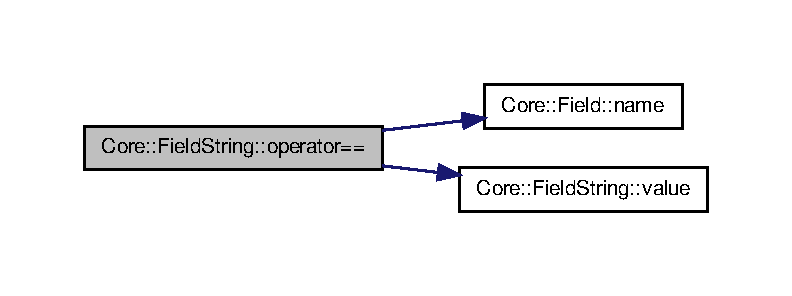
\includegraphics[width=380pt]{dd/d02/classCore_1_1FieldString_adacfe0012314f6840b2657d63ffe8c49_cgraph}
\end{center}
\end{figure}


\hypertarget{classCore_1_1FieldString_a1cf5a18e64379806684e0bb110a002d1}{
\index{Core::FieldString@{Core::FieldString}!value@{value}}
\index{value@{value}!Core::FieldString@{Core::FieldString}}
\subsubsection[{value}]{\setlength{\rightskip}{0pt plus 5cm}const std::string\& Core::FieldString::value (
\begin{DoxyParamCaption}
\item[{const std::string \&}]{value}
\end{DoxyParamCaption}
)  throw ()\hspace{0.3cm}{\ttfamily  \mbox{[}inline\mbox{]}}}}
\label{dd/d02/classCore_1_1FieldString_a1cf5a18e64379806684e0bb110a002d1}


Change value. 

$<$ 
\begin{DoxyParams}[1]{Parameters}
\mbox{\tt in}  & {\em New} & value of the field. \\
\hline
\end{DoxyParams}
\begin{DoxyReturn}{Returns}
Value of the field AFTER assigment. 
\end{DoxyReturn}


Here is the call graph for this function:
\nopagebreak
\begin{figure}[H]
\begin{center}
\leavevmode
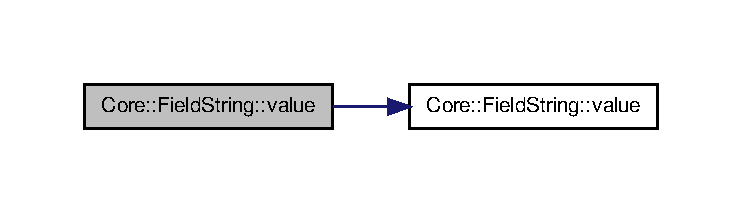
\includegraphics[width=356pt]{dd/d02/classCore_1_1FieldString_a1cf5a18e64379806684e0bb110a002d1_cgraph}
\end{center}
\end{figure}


\hypertarget{classCore_1_1FieldString_a31f2a21becad6221f033daaf8aa161d7}{
\index{Core::FieldString@{Core::FieldString}!value@{value}}
\index{value@{value}!Core::FieldString@{Core::FieldString}}
\subsubsection[{value}]{\setlength{\rightskip}{0pt plus 5cm}const std::string\& Core::FieldString::value (
\begin{DoxyParamCaption}
{}
\end{DoxyParamCaption}
) const  throw ()\hspace{0.3cm}{\ttfamily  \mbox{[}inline\mbox{]}}}}
\label{dd/d02/classCore_1_1FieldString_a31f2a21becad6221f033daaf8aa161d7}


Get value. 

$<$ \begin{DoxyReturn}{Returns}
Current value of the field.
\end{DoxyReturn}
This method does not changes value. 

Here is the caller graph for this function:
\nopagebreak
\begin{figure}[H]
\begin{center}
\leavevmode
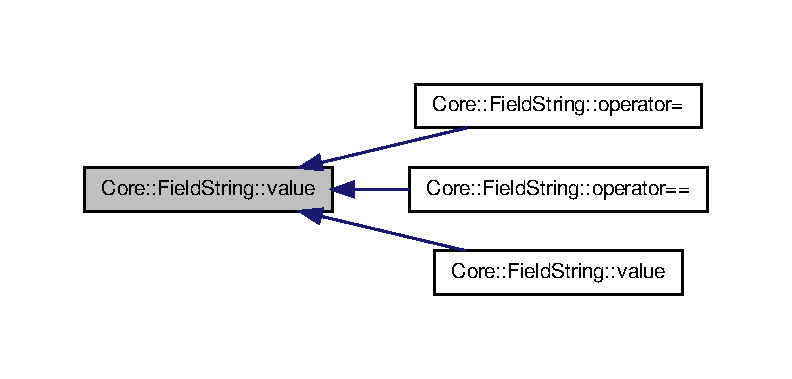
\includegraphics[width=380pt]{dd/d02/classCore_1_1FieldString_a31f2a21becad6221f033daaf8aa161d7_icgraph}
\end{center}
\end{figure}




The documentation for this class was generated from the following file:\begin{DoxyCompactItemize}
\item 
src/include/\hyperlink{field_8h}{field.h}\end{DoxyCompactItemize}

\hypertarget{classCore_1_1FieldTime}{
\section{Core::FieldTime Class Reference}
\label{d3/d8b/classCore_1_1FieldTime}\index{Core::FieldTime@{Core::FieldTime}}
}


field of time\_\-t type.  




{\ttfamily \#include $<$field.h$>$}



Inheritance diagram for Core::FieldTime:
\nopagebreak
\begin{figure}[H]
\begin{center}
\leavevmode
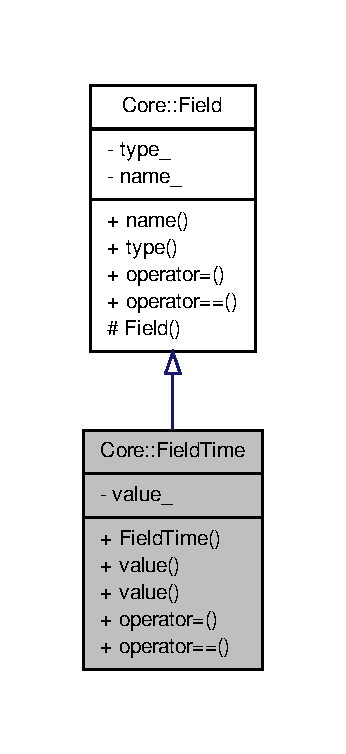
\includegraphics[width=166pt]{d7/d6a/classCore_1_1FieldTime__inherit__graph}
\end{center}
\end{figure}


Collaboration diagram for Core::FieldTime:
\nopagebreak
\begin{figure}[H]
\begin{center}
\leavevmode
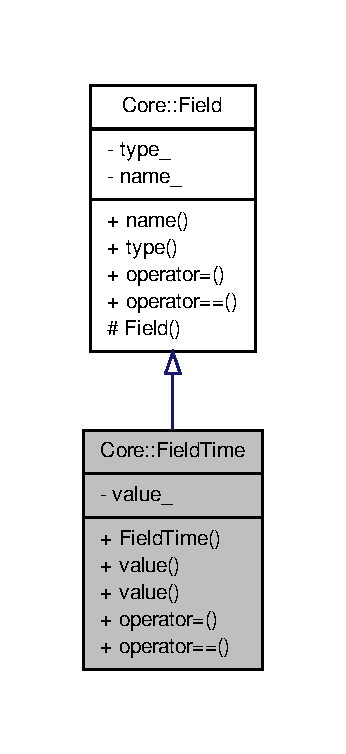
\includegraphics[width=166pt]{d7/d8c/classCore_1_1FieldTime__coll__graph}
\end{center}
\end{figure}
\subsection*{Public Member Functions}
\begin{DoxyCompactItemize}
\item 
\hyperlink{classCore_1_1FieldTime_ad1b0b00de785462e57fd625d1ef6beb6}{FieldTime} (const std::string \&name, const time\_\-t \&value=0)  throw ()
\begin{DoxyCompactList}\small\item\em Constructor. \item\end{DoxyCompactList}\item 
const time\_\-t \hyperlink{classCore_1_1FieldTime_aeaf4283ac92d2a718d6225a717073a17}{value} (const time\_\-t \&value)  throw ()
\item 
const time\_\-t \hyperlink{classCore_1_1FieldTime_aca53dd5590b476699aeb670068b4592e}{value} () const   throw ()
\item 
virtual const \hyperlink{classCore_1_1Field}{Field} \& \hyperlink{classCore_1_1FieldTime_ab0b9e7fe5ee619d3d584dfd3a9be5015}{operator=} (const \hyperlink{classCore_1_1Field}{Field} \&field)  throw (std::bad\_\-cast)
\item 
virtual const bool \hyperlink{classCore_1_1FieldTime_aa48c2e4d7c6ad13794f66f3e59849843}{operator==} (const \hyperlink{classCore_1_1Field}{Field} \&field) const   throw (std::bad\_\-cast)
\end{DoxyCompactItemize}


\subsection{Detailed Description}
field of time\_\-t type. Simple class contains name and time\_\-t value. 

\subsection{Constructor \& Destructor Documentation}
\hypertarget{classCore_1_1FieldTime_ad1b0b00de785462e57fd625d1ef6beb6}{
\index{Core::FieldTime@{Core::FieldTime}!FieldTime@{FieldTime}}
\index{FieldTime@{FieldTime}!Core::FieldTime@{Core::FieldTime}}
\subsubsection[{FieldTime}]{\setlength{\rightskip}{0pt plus 5cm}Core::FieldTime::FieldTime (
\begin{DoxyParamCaption}
\item[{const std::string \&}]{name, }
\item[{const time\_\-t \&}]{value = {\ttfamily 0}}
\end{DoxyParamCaption}
)  throw ()\hspace{0.3cm}{\ttfamily  \mbox{[}inline\mbox{]}}}}
\label{d3/d8b/classCore_1_1FieldTime_ad1b0b00de785462e57fd625d1ef6beb6}


Constructor. 

$<$ 
\begin{DoxyParams}[1]{Parameters}
\mbox{\tt in}  & {\em name} & Name of the field. \\
\hline
\mbox{\tt in}  & {\em value} & Value of the field. Zero by default. \\
\hline
\end{DoxyParams}


\subsection{Member Function Documentation}
\hypertarget{classCore_1_1FieldTime_ab0b9e7fe5ee619d3d584dfd3a9be5015}{
\index{Core::FieldTime@{Core::FieldTime}!operator=@{operator=}}
\index{operator=@{operator=}!Core::FieldTime@{Core::FieldTime}}
\subsubsection[{operator=}]{\setlength{\rightskip}{0pt plus 5cm}virtual const {\bf Field}\& Core::FieldTime::operator= (
\begin{DoxyParamCaption}
\item[{const {\bf Field} \&}]{field}
\end{DoxyParamCaption}
)  throw (std::bad\_\-cast)\hspace{0.3cm}{\ttfamily  \mbox{[}inline, virtual\mbox{]}}}}
\label{d3/d8b/classCore_1_1FieldTime_ab0b9e7fe5ee619d3d584dfd3a9be5015}
$<$ Assigment operator. 


\begin{DoxyParams}[1]{Parameters}
\mbox{\tt in}  & {\em field} & \hyperlink{classCore_1_1Field}{Field} with value to assign. \\
\hline
\end{DoxyParams}
\begin{DoxyReturn}{Returns}
This field.
\end{DoxyReturn}
Assign this field's value to another fields value, if they have one type.  Implementation for time\_\-t type. 

Implements \hyperlink{classCore_1_1Field_a3300f5867380b0e55bcd6c1918815e1f}{Core::Field}.



Here is the call graph for this function:
\nopagebreak
\begin{figure}[H]
\begin{center}
\leavevmode
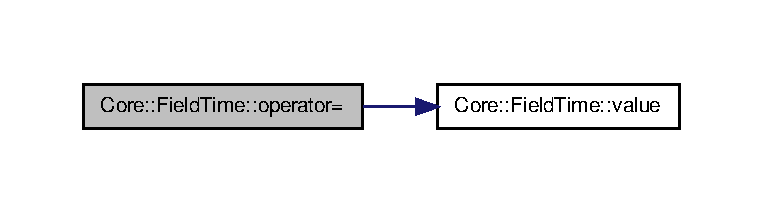
\includegraphics[width=366pt]{d3/d8b/classCore_1_1FieldTime_ab0b9e7fe5ee619d3d584dfd3a9be5015_cgraph}
\end{center}
\end{figure}


\hypertarget{classCore_1_1FieldTime_aa48c2e4d7c6ad13794f66f3e59849843}{
\index{Core::FieldTime@{Core::FieldTime}!operator==@{operator==}}
\index{operator==@{operator==}!Core::FieldTime@{Core::FieldTime}}
\subsubsection[{operator==}]{\setlength{\rightskip}{0pt plus 5cm}virtual const bool Core::FieldTime::operator== (
\begin{DoxyParamCaption}
\item[{const {\bf Field} \&}]{field}
\end{DoxyParamCaption}
) const  throw (std::bad\_\-cast)\hspace{0.3cm}{\ttfamily  \mbox{[}inline, virtual\mbox{]}}}}
\label{d3/d8b/classCore_1_1FieldTime_aa48c2e4d7c6ad13794f66f3e59849843}
$<$ Comparison operator. 


\begin{DoxyParams}[1]{Parameters}
\mbox{\tt in}  & {\em field} & \hyperlink{classCore_1_1Field}{Field} with value to compare. \\
\hline
\end{DoxyParams}
\begin{DoxyReturn}{Returns}
result of comparison.
\end{DoxyReturn}
Compare values of two fields, if they have one type.  Implementation for time\_\-t type. 

Implements \hyperlink{classCore_1_1Field_ae2db5ff861ee23a5d5cc43913544a4ab}{Core::Field}.



Here is the call graph for this function:
\nopagebreak
\begin{figure}[H]
\begin{center}
\leavevmode
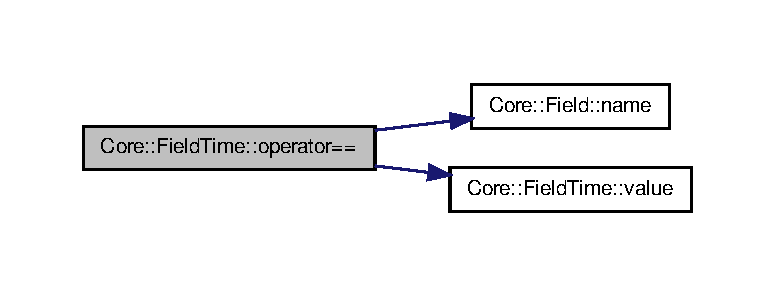
\includegraphics[width=372pt]{d3/d8b/classCore_1_1FieldTime_aa48c2e4d7c6ad13794f66f3e59849843_cgraph}
\end{center}
\end{figure}


\hypertarget{classCore_1_1FieldTime_aeaf4283ac92d2a718d6225a717073a17}{
\index{Core::FieldTime@{Core::FieldTime}!value@{value}}
\index{value@{value}!Core::FieldTime@{Core::FieldTime}}
\subsubsection[{value}]{\setlength{\rightskip}{0pt plus 5cm}const time\_\-t Core::FieldTime::value (
\begin{DoxyParamCaption}
\item[{const time\_\-t \&}]{value}
\end{DoxyParamCaption}
)  throw ()\hspace{0.3cm}{\ttfamily  \mbox{[}inline\mbox{]}}}}
\label{d3/d8b/classCore_1_1FieldTime_aeaf4283ac92d2a718d6225a717073a17}
$<$  

Here is the call graph for this function:
\nopagebreak
\begin{figure}[H]
\begin{center}
\leavevmode
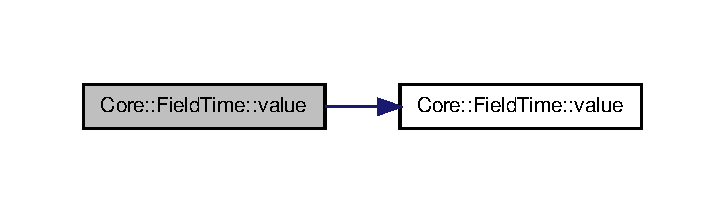
\includegraphics[width=348pt]{d3/d8b/classCore_1_1FieldTime_aeaf4283ac92d2a718d6225a717073a17_cgraph}
\end{center}
\end{figure}


\hypertarget{classCore_1_1FieldTime_aca53dd5590b476699aeb670068b4592e}{
\index{Core::FieldTime@{Core::FieldTime}!value@{value}}
\index{value@{value}!Core::FieldTime@{Core::FieldTime}}
\subsubsection[{value}]{\setlength{\rightskip}{0pt plus 5cm}const time\_\-t Core::FieldTime::value (
\begin{DoxyParamCaption}
{}
\end{DoxyParamCaption}
) const  throw ()\hspace{0.3cm}{\ttfamily  \mbox{[}inline\mbox{]}}}}
\label{d3/d8b/classCore_1_1FieldTime_aca53dd5590b476699aeb670068b4592e}
$<$ Change value. 

$<$ 
\begin{DoxyParams}[1]{Parameters}
\mbox{\tt in}  & {\em New} & value of the field. \\
\hline
\end{DoxyParams}
\begin{DoxyReturn}{Returns}
Value of the field AFTER assigment. 
\end{DoxyReturn}
 

Here is the caller graph for this function:
\nopagebreak
\begin{figure}[H]
\begin{center}
\leavevmode
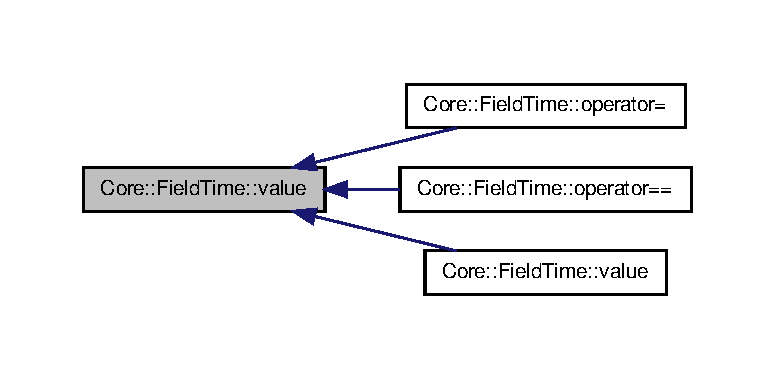
\includegraphics[width=372pt]{d3/d8b/classCore_1_1FieldTime_aca53dd5590b476699aeb670068b4592e_icgraph}
\end{center}
\end{figure}




The documentation for this class was generated from the following file:\begin{DoxyCompactItemize}
\item 
src/include/\hyperlink{field_8h}{field.h}\end{DoxyCompactItemize}

\hypertarget{classCore_1_1FieldVector}{
\section{Core::FieldVector Class Reference}
\label{dc/d7f/classCore_1_1FieldVector}\index{Core::FieldVector@{Core::FieldVector}}
}


\hyperlink{classCore_1_1Field}{Field} of vector type.  




{\ttfamily \#include $<$field.h$>$}



Inheritance diagram for Core::FieldVector:
\nopagebreak
\begin{figure}[H]
\begin{center}
\leavevmode
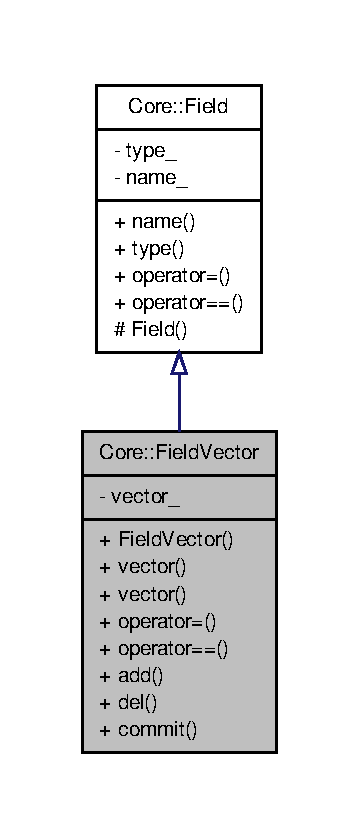
\includegraphics[width=172pt]{d9/d80/classCore_1_1FieldVector__inherit__graph}
\end{center}
\end{figure}


Collaboration diagram for Core::FieldVector:
\nopagebreak
\begin{figure}[H]
\begin{center}
\leavevmode
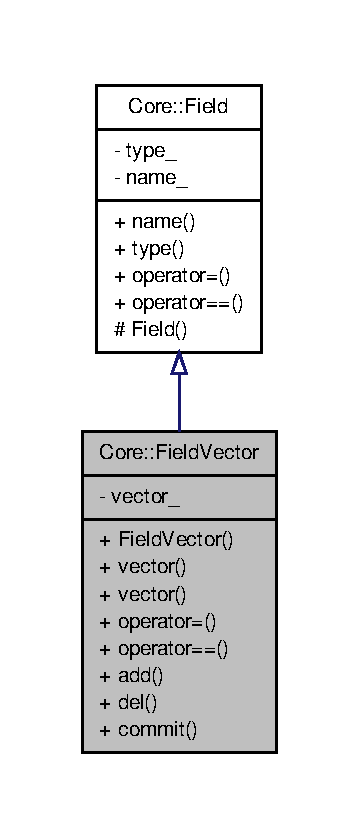
\includegraphics[width=172pt]{d8/d31/classCore_1_1FieldVector__coll__graph}
\end{center}
\end{figure}
\subsection*{Public Member Functions}
\begin{DoxyCompactItemize}
\item 
\hyperlink{classCore_1_1FieldVector_ae0a35cb365468b2434527ecff44bff9d}{FieldVector} (const std::string \&name, const std::vector$<$ \hyperlink{classCore_1_1Object}{Object} $\ast$ $>$ \&vector=std::vector$<$ \hyperlink{classCore_1_1Object}{Object} $\ast$ $>$())  throw ()
\begin{DoxyCompactList}\small\item\em Constructor. \item\end{DoxyCompactList}\item 
const std::vector$<$ \hyperlink{classCore_1_1Object}{Object} $\ast$ $>$ \& \hyperlink{classCore_1_1FieldVector_ae2855da313c104367b35b97eb98097dc}{vector} (const std::vector$<$ \hyperlink{classCore_1_1Object}{Object} $\ast$ $>$ \&vector)  throw ()
\begin{DoxyCompactList}\small\item\em Change vector. \item\end{DoxyCompactList}\item 
const std::vector$<$ \hyperlink{classCore_1_1Object}{Object} $\ast$ $>$ \& \hyperlink{classCore_1_1FieldVector_a75f050f282ad9848aceae2efbb9d72cd}{vector} () const   throw ()
\begin{DoxyCompactList}\small\item\em Get vector. \item\end{DoxyCompactList}\item 
virtual const \hyperlink{classCore_1_1Field}{Field} \& \hyperlink{classCore_1_1FieldVector_a8482c272e2bc4e5b09194b903bead7f7}{operator=} (const \hyperlink{classCore_1_1Field}{Field} \&field)  throw (std::bad\_\-cast)
\item 
virtual const bool \hyperlink{classCore_1_1FieldVector_a79df85b6378b5ce608ca579bd3e23027}{operator==} (const \hyperlink{classCore_1_1Field}{Field} \&field) const   throw (std::bad\_\-cast)
\item 
void \hyperlink{classCore_1_1FieldVector_ab99c7d1efa922626c965378513eea97c}{add} (\hyperlink{classCore_1_1Object}{Object} $\ast$object)
\item 
void \hyperlink{classCore_1_1FieldVector_a998eb9129eab985880411f7c564879d3}{del} (\hyperlink{classCore_1_1Object}{Object} $\ast$object)
\item 
void \hyperlink{classCore_1_1FieldVector_a62af016fcb50e445db4ad64123281106}{commit} (const \hyperlink{classCore_1_1FieldLink}{FieldLink} \&field)
\end{DoxyCompactItemize}


\subsection{Detailed Description}
\hyperlink{classCore_1_1Field}{Field} of vector type. Class contains name and std::vector$<$Object $\ast$$>$ vector. 

\subsection{Constructor \& Destructor Documentation}
\hypertarget{classCore_1_1FieldVector_ae0a35cb365468b2434527ecff44bff9d}{
\index{Core::FieldVector@{Core::FieldVector}!FieldVector@{FieldVector}}
\index{FieldVector@{FieldVector}!Core::FieldVector@{Core::FieldVector}}
\subsubsection[{FieldVector}]{\setlength{\rightskip}{0pt plus 5cm}Core::FieldVector::FieldVector (
\begin{DoxyParamCaption}
\item[{const std::string \&}]{name, }
\item[{const std::vector$<$ {\bf Object} $\ast$ $>$ \&}]{vector = {\ttfamily std::vector$<${\bf Object}~$\ast$$>$()}}
\end{DoxyParamCaption}
)  throw ()\hspace{0.3cm}{\ttfamily  \mbox{[}inline\mbox{]}}}}
\label{dc/d7f/classCore_1_1FieldVector_ae0a35cb365468b2434527ecff44bff9d}


Constructor. 

$<$ 
\begin{DoxyParams}[1]{Parameters}
\mbox{\tt in}  & {\em name} & Name of the field. \\
\hline
\mbox{\tt in}  & {\em vector} & Vector of the objects. Empty by default. \\
\hline
\end{DoxyParams}


\subsection{Member Function Documentation}
\hypertarget{classCore_1_1FieldVector_ab99c7d1efa922626c965378513eea97c}{
\index{Core::FieldVector@{Core::FieldVector}!add@{add}}
\index{add@{add}!Core::FieldVector@{Core::FieldVector}}
\subsubsection[{add}]{\setlength{\rightskip}{0pt plus 5cm}void Core::FieldVector::add (
\begin{DoxyParamCaption}
\item[{{\bf Object} $\ast$}]{object}
\end{DoxyParamCaption}
)\hspace{0.3cm}{\ttfamily  \mbox{[}inline\mbox{]}}}}
\label{dc/d7f/classCore_1_1FieldVector_ab99c7d1efa922626c965378513eea97c}

\begin{DoxyParams}[1]{Parameters}
 & {\em object} & Add object to the vector. \\
\hline
\mbox{\tt in}  & {\em object} & \hyperlink{classCore_1_1Object}{Object} to add. \\
\hline
\end{DoxyParams}


Here is the caller graph for this function:
\nopagebreak
\begin{figure}[H]
\begin{center}
\leavevmode
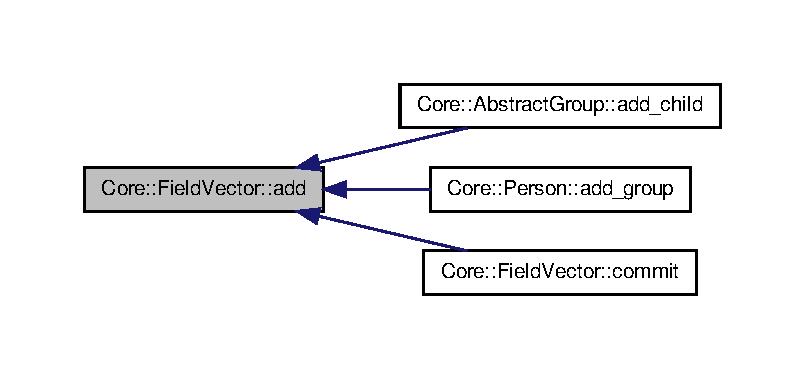
\includegraphics[width=386pt]{dc/d7f/classCore_1_1FieldVector_ab99c7d1efa922626c965378513eea97c_icgraph}
\end{center}
\end{figure}


\hypertarget{classCore_1_1FieldVector_a62af016fcb50e445db4ad64123281106}{
\index{Core::FieldVector@{Core::FieldVector}!commit@{commit}}
\index{commit@{commit}!Core::FieldVector@{Core::FieldVector}}
\subsubsection[{commit}]{\setlength{\rightskip}{0pt plus 5cm}void Core::FieldVector::commit (
\begin{DoxyParamCaption}
\item[{const {\bf FieldLink} \&}]{field}
\end{DoxyParamCaption}
)\hspace{0.3cm}{\ttfamily  \mbox{[}inline\mbox{]}}}}
\label{dc/d7f/classCore_1_1FieldVector_a62af016fcb50e445db4ad64123281106}

\begin{DoxyParams}[1]{Parameters}
 & {\em field} & apply link to the vector. \\
\hline
\mbox{\tt in}  & {\em field} & Link to apply. \\
\hline
\end{DoxyParams}


Here is the call graph for this function:
\nopagebreak
\begin{figure}[H]
\begin{center}
\leavevmode
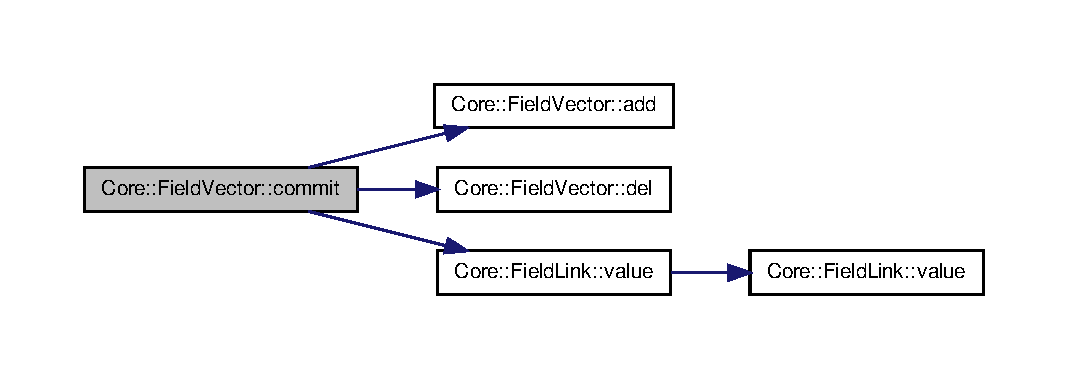
\includegraphics[width=400pt]{dc/d7f/classCore_1_1FieldVector_a62af016fcb50e445db4ad64123281106_cgraph}
\end{center}
\end{figure}


\hypertarget{classCore_1_1FieldVector_a998eb9129eab985880411f7c564879d3}{
\index{Core::FieldVector@{Core::FieldVector}!del@{del}}
\index{del@{del}!Core::FieldVector@{Core::FieldVector}}
\subsubsection[{del}]{\setlength{\rightskip}{0pt plus 5cm}void Core::FieldVector::del (
\begin{DoxyParamCaption}
\item[{{\bf Object} $\ast$}]{object}
\end{DoxyParamCaption}
)\hspace{0.3cm}{\ttfamily  \mbox{[}inline\mbox{]}}}}
\label{dc/d7f/classCore_1_1FieldVector_a998eb9129eab985880411f7c564879d3}

\begin{DoxyParams}[1]{Parameters}
 & {\em object} & Delete object to the vector. \\
\hline
\mbox{\tt in}  & {\em object} & \hyperlink{classCore_1_1Object}{Object} to delete. \\
\hline
\end{DoxyParams}


Here is the caller graph for this function:
\nopagebreak
\begin{figure}[H]
\begin{center}
\leavevmode
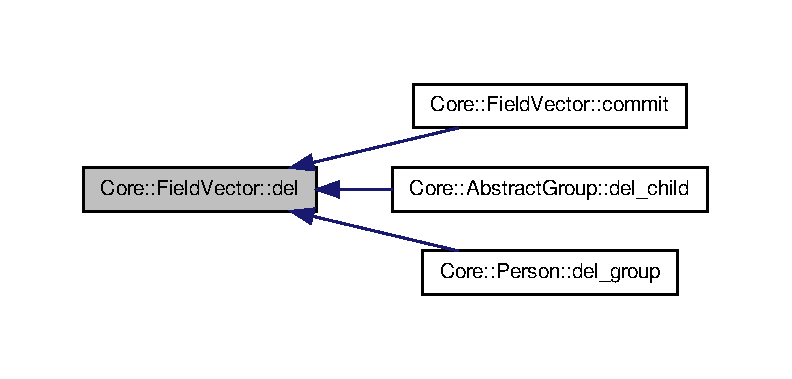
\includegraphics[width=380pt]{dc/d7f/classCore_1_1FieldVector_a998eb9129eab985880411f7c564879d3_icgraph}
\end{center}
\end{figure}


\hypertarget{classCore_1_1FieldVector_a8482c272e2bc4e5b09194b903bead7f7}{
\index{Core::FieldVector@{Core::FieldVector}!operator=@{operator=}}
\index{operator=@{operator=}!Core::FieldVector@{Core::FieldVector}}
\subsubsection[{operator=}]{\setlength{\rightskip}{0pt plus 5cm}virtual const {\bf Field}\& Core::FieldVector::operator= (
\begin{DoxyParamCaption}
\item[{const {\bf Field} \&}]{field}
\end{DoxyParamCaption}
)  throw (std::bad\_\-cast)\hspace{0.3cm}{\ttfamily  \mbox{[}inline, virtual\mbox{]}}}}
\label{dc/d7f/classCore_1_1FieldVector_a8482c272e2bc4e5b09194b903bead7f7}
$<$ Assigment operator. 


\begin{DoxyParams}[1]{Parameters}
\mbox{\tt in}  & {\em field} & \hyperlink{classCore_1_1Field}{Field} with value to assign. \\
\hline
\end{DoxyParams}
\begin{DoxyReturn}{Returns}
This field.
\end{DoxyReturn}
Assign this field's value to another fields value, if they have one type.  

Implements \hyperlink{classCore_1_1Field_a3300f5867380b0e55bcd6c1918815e1f}{Core::Field}.



Here is the call graph for this function:
\nopagebreak
\begin{figure}[H]
\begin{center}
\leavevmode
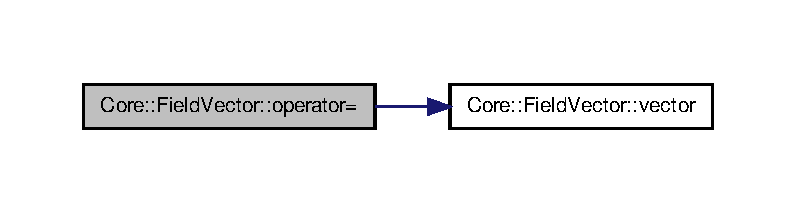
\includegraphics[width=382pt]{dc/d7f/classCore_1_1FieldVector_a8482c272e2bc4e5b09194b903bead7f7_cgraph}
\end{center}
\end{figure}


\hypertarget{classCore_1_1FieldVector_a79df85b6378b5ce608ca579bd3e23027}{
\index{Core::FieldVector@{Core::FieldVector}!operator==@{operator==}}
\index{operator==@{operator==}!Core::FieldVector@{Core::FieldVector}}
\subsubsection[{operator==}]{\setlength{\rightskip}{0pt plus 5cm}virtual const bool Core::FieldVector::operator== (
\begin{DoxyParamCaption}
\item[{const {\bf Field} \&}]{field}
\end{DoxyParamCaption}
) const  throw (std::bad\_\-cast)\hspace{0.3cm}{\ttfamily  \mbox{[}inline, virtual\mbox{]}}}}
\label{dc/d7f/classCore_1_1FieldVector_a79df85b6378b5ce608ca579bd3e23027}
$<$ Comparison operator. 


\begin{DoxyParams}[1]{Parameters}
\mbox{\tt in}  & {\em field} & \hyperlink{classCore_1_1Field}{Field} with value to compare. \\
\hline
\end{DoxyParams}
\begin{DoxyReturn}{Returns}
result of comparison.
\end{DoxyReturn}
Compare values of two fields, if they have one type.  

Implements \hyperlink{classCore_1_1Field_ae2db5ff861ee23a5d5cc43913544a4ab}{Core::Field}.

\hypertarget{classCore_1_1FieldVector_ae2855da313c104367b35b97eb98097dc}{
\index{Core::FieldVector@{Core::FieldVector}!vector@{vector}}
\index{vector@{vector}!Core::FieldVector@{Core::FieldVector}}
\subsubsection[{vector}]{\setlength{\rightskip}{0pt plus 5cm}const std::vector$<${\bf Object} $\ast$$>$\& Core::FieldVector::vector (
\begin{DoxyParamCaption}
\item[{const std::vector$<$ {\bf Object} $\ast$ $>$ \&}]{vector}
\end{DoxyParamCaption}
)  throw ()\hspace{0.3cm}{\ttfamily  \mbox{[}inline\mbox{]}}}}
\label{dc/d7f/classCore_1_1FieldVector_ae2855da313c104367b35b97eb98097dc}


Change vector. 

$<$ 
\begin{DoxyParams}[1]{Parameters}
\mbox{\tt in}  & {\em vector} & New vector. \\
\hline
\end{DoxyParams}
\begin{DoxyReturn}{Returns}
Vector AFTER assigment. 
\end{DoxyReturn}


Here is the call graph for this function:
\nopagebreak
\begin{figure}[H]
\begin{center}
\leavevmode
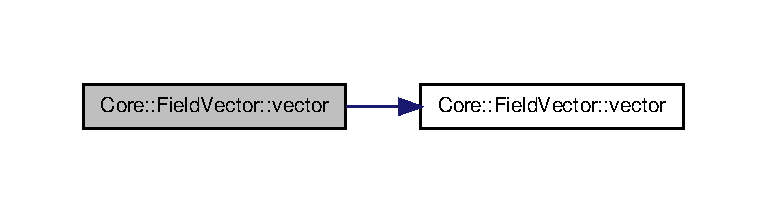
\includegraphics[width=368pt]{dc/d7f/classCore_1_1FieldVector_ae2855da313c104367b35b97eb98097dc_cgraph}
\end{center}
\end{figure}


\hypertarget{classCore_1_1FieldVector_a75f050f282ad9848aceae2efbb9d72cd}{
\index{Core::FieldVector@{Core::FieldVector}!vector@{vector}}
\index{vector@{vector}!Core::FieldVector@{Core::FieldVector}}
\subsubsection[{vector}]{\setlength{\rightskip}{0pt plus 5cm}const std::vector$<${\bf Object} $\ast$$>$\& Core::FieldVector::vector (
\begin{DoxyParamCaption}
{}
\end{DoxyParamCaption}
) const  throw ()\hspace{0.3cm}{\ttfamily  \mbox{[}inline\mbox{]}}}}
\label{dc/d7f/classCore_1_1FieldVector_a75f050f282ad9848aceae2efbb9d72cd}


Get vector. 

$<$ \begin{DoxyReturn}{Returns}
Current vector.
\end{DoxyReturn}
This method does not change the vector. 

Here is the caller graph for this function:
\nopagebreak
\begin{figure}[H]
\begin{center}
\leavevmode
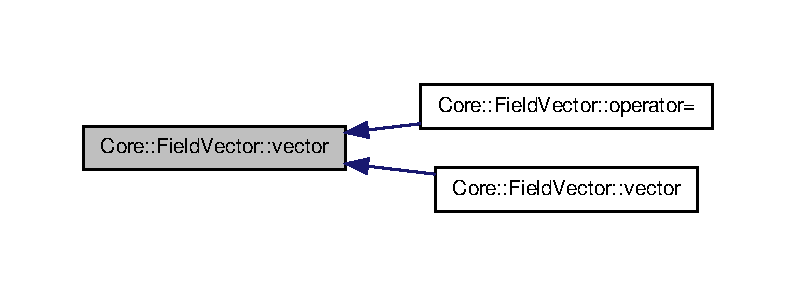
\includegraphics[width=382pt]{dc/d7f/classCore_1_1FieldVector_a75f050f282ad9848aceae2efbb9d72cd_icgraph}
\end{center}
\end{figure}




The documentation for this class was generated from the following file:\begin{DoxyCompactItemize}
\item 
src/include/\hyperlink{field_8h}{field.h}\end{DoxyCompactItemize}

\hypertarget{classCore_1_1Group}{
\section{Core::Group Class Reference}
\label{d2/d30/classCore_1_1Group}\index{Core::Group@{Core::Group}}
}


Class keeps information about group of people.  




{\ttfamily \#include $<$group.h$>$}



Inheritance diagram for Core::Group:
\nopagebreak
\begin{figure}[H]
\begin{center}
\leavevmode
\includegraphics[height=600pt]{d6/d15/classCore_1_1Group__inherit__graph}
\end{center}
\end{figure}


Collaboration diagram for Core::Group:
\nopagebreak
\begin{figure}[H]
\begin{center}
\leavevmode
\includegraphics[height=600pt]{d7/da7/classCore_1_1Group__coll__graph}
\end{center}
\end{figure}
\subsection*{Public Member Functions}
\begin{DoxyCompactItemize}
\item 
\hyperlink{classCore_1_1Group_a39511a091570283cb5fb2a4b8f0a841a}{Group} (const int id, \hyperlink{classStorage_1_1AbstractStorage}{Storage::AbstractStorage} \&storage)
\item 
void \hyperlink{classCore_1_1Group_a05760e4e45ae6fec2674d216f0a5a6e9}{add\_\-parent\_\-group} (\hyperlink{classCore_1_1AbstractGroup}{AbstractGroup} $\ast$group)
\item 
void \hyperlink{classCore_1_1Group_a93e4626dde0f84e68f1460e557daaed0}{del\_\-parent\_\-group} (\hyperlink{classCore_1_1AbstractGroup}{AbstractGroup} $\ast$group)
\item 
virtual const std::string \hyperlink{classCore_1_1Group_a5fe3fef1b6709f953e5487841d90bbb9}{read} () const 
\begin{DoxyCompactList}\small\item\em Returns full object information. \item\end{DoxyCompactList}\item 
virtual const std::vector$<$ \hyperlink{classUI_1_1UsersObject}{UI::UsersObject} $\ast$ $>$ \hyperlink{classCore_1_1Group_a52e48b1f92f6354b4e3a32d710b9c7b3}{read\_\-vector} (const std::string name) const   throw (std::bad\_\-cast)
\begin{DoxyCompactList}\small\item\em Return vector value of requested field. \item\end{DoxyCompactList}\item 
virtual void \hyperlink{classCore_1_1Group_a12d2636d65f1baea3666bb492320b5c1}{update} (\hyperlink{classUI_1_1UsersObject}{UI::UsersObject} $\ast$object, const bool linked)  throw (std::bad\_\-cast)
\begin{DoxyCompactList}\small\item\em change current link value of field. \item\end{DoxyCompactList}\end{DoxyCompactItemize}


\subsection{Detailed Description}
Class keeps information about group of people. $<$ 

\subsection{Constructor \& Destructor Documentation}
\hypertarget{classCore_1_1Group_a39511a091570283cb5fb2a4b8f0a841a}{
\index{Core::Group@{Core::Group}!Group@{Group}}
\index{Group@{Group}!Core::Group@{Core::Group}}
\subsubsection[{Group}]{\setlength{\rightskip}{0pt plus 5cm}Core::Group::Group (
\begin{DoxyParamCaption}
\item[{const int}]{id, }
\item[{{\bf Storage::AbstractStorage} \&}]{storage}
\end{DoxyParamCaption}
)\hspace{0.3cm}{\ttfamily  \mbox{[}inline\mbox{]}}}}
\label{d2/d30/classCore_1_1Group_a39511a091570283cb5fb2a4b8f0a841a}


\subsection{Member Function Documentation}
\hypertarget{classCore_1_1Group_a05760e4e45ae6fec2674d216f0a5a6e9}{
\index{Core::Group@{Core::Group}!add\_\-parent\_\-group@{add\_\-parent\_\-group}}
\index{add\_\-parent\_\-group@{add\_\-parent\_\-group}!Core::Group@{Core::Group}}
\subsubsection[{add\_\-parent\_\-group}]{\setlength{\rightskip}{0pt plus 5cm}void Group::add\_\-parent\_\-group (
\begin{DoxyParamCaption}
\item[{{\bf AbstractGroup} $\ast$}]{group}
\end{DoxyParamCaption}
)}}
\label{d2/d30/classCore_1_1Group_a05760e4e45ae6fec2674d216f0a5a6e9}


Here is the call graph for this function:
\nopagebreak
\begin{figure}[H]
\begin{center}
\leavevmode
\includegraphics[width=400pt]{d2/d30/classCore_1_1Group_a05760e4e45ae6fec2674d216f0a5a6e9_cgraph}
\end{center}
\end{figure}


\hypertarget{classCore_1_1Group_a93e4626dde0f84e68f1460e557daaed0}{
\index{Core::Group@{Core::Group}!del\_\-parent\_\-group@{del\_\-parent\_\-group}}
\index{del\_\-parent\_\-group@{del\_\-parent\_\-group}!Core::Group@{Core::Group}}
\subsubsection[{del\_\-parent\_\-group}]{\setlength{\rightskip}{0pt plus 5cm}void Group::del\_\-parent\_\-group (
\begin{DoxyParamCaption}
\item[{{\bf AbstractGroup} $\ast$}]{group}
\end{DoxyParamCaption}
)}}
\label{d2/d30/classCore_1_1Group_a93e4626dde0f84e68f1460e557daaed0}


Here is the call graph for this function:
\nopagebreak
\begin{figure}[H]
\begin{center}
\leavevmode
\includegraphics[width=400pt]{d2/d30/classCore_1_1Group_a93e4626dde0f84e68f1460e557daaed0_cgraph}
\end{center}
\end{figure}


\hypertarget{classCore_1_1Group_a5fe3fef1b6709f953e5487841d90bbb9}{
\index{Core::Group@{Core::Group}!read@{read}}
\index{read@{read}!Core::Group@{Core::Group}}
\subsubsection[{read}]{\setlength{\rightskip}{0pt plus 5cm}const std::string Group::read (
\begin{DoxyParamCaption}
{}
\end{DoxyParamCaption}
) const\hspace{0.3cm}{\ttfamily  \mbox{[}virtual\mbox{]}}}}
\label{d2/d30/classCore_1_1Group_a5fe3fef1b6709f953e5487841d90bbb9}


Returns full object information. 

\begin{DoxyReturn}{Returns}
Object`s information in the string.
\end{DoxyReturn}
Method declared in the \hyperlink{classUI_1_1UsersObject}{UI::UsersObject} use to retrive all information about object.

Inherited classes must to redefine and call this one. 

Reimplemented from \hyperlink{classCore_1_1AbstractGroup_a0306b58e715d164aef3e29de0ec659bd}{Core::AbstractGroup}.

\hypertarget{classCore_1_1Group_a52e48b1f92f6354b4e3a32d710b9c7b3}{
\index{Core::Group@{Core::Group}!read\_\-vector@{read\_\-vector}}
\index{read\_\-vector@{read\_\-vector}!Core::Group@{Core::Group}}
\subsubsection[{read\_\-vector}]{\setlength{\rightskip}{0pt plus 5cm}const std::vector$<$ {\bf UI::UsersObject} $\ast$ $>$ Group::read\_\-vector (
\begin{DoxyParamCaption}
\item[{const std::string}]{name}
\end{DoxyParamCaption}
) const  throw (std::bad\_\-cast)\hspace{0.3cm}{\ttfamily  \mbox{[}virtual\mbox{]}}}}
\label{d2/d30/classCore_1_1Group_a52e48b1f92f6354b4e3a32d710b9c7b3}


Return vector value of requested field. 


\begin{DoxyParams}{Parameters}
{\em name} & Name of field which must be returned. \\
\hline
\end{DoxyParams}
\begin{DoxyReturn}{Returns}
Vector value of requested field.
\end{DoxyReturn}
Use this for child\_\-groups and people fields. Throws exception in the other cases. 

Reimplemented from \hyperlink{classCore_1_1AbstractGroup_ab582f4364426a152875742278ba0d999}{Core::AbstractGroup}.



Here is the call graph for this function:
\nopagebreak
\begin{figure}[H]
\begin{center}
\leavevmode
\includegraphics[width=400pt]{d2/d30/classCore_1_1Group_a52e48b1f92f6354b4e3a32d710b9c7b3_cgraph}
\end{center}
\end{figure}


\hypertarget{classCore_1_1Group_a12d2636d65f1baea3666bb492320b5c1}{
\index{Core::Group@{Core::Group}!update@{update}}
\index{update@{update}!Core::Group@{Core::Group}}
\subsubsection[{update}]{\setlength{\rightskip}{0pt plus 5cm}void Group::update (
\begin{DoxyParamCaption}
\item[{{\bf UI::UsersObject} $\ast$}]{object, }
\item[{const bool}]{linked}
\end{DoxyParamCaption}
)  throw (std::bad\_\-cast)\hspace{0.3cm}{\ttfamily  \mbox{[}virtual\mbox{]}}}}
\label{d2/d30/classCore_1_1Group_a12d2636d65f1baea3666bb492320b5c1}


change current link value of field. 


\begin{DoxyParams}{Parameters}
{\em object} & Object link with that must be changed. \\
\hline
{\em linked} & New state of thi link.\\
\hline
\end{DoxyParams}
This method tries to add or delete object to the group as the \hyperlink{classCore_1_1Person}{Person}. dynamic\_\-cast will throw std::bad\_\-cast if object is not \hyperlink{classCore_1_1Person}{Person}.

You can not set child group by this method use redefined method in \hyperlink{classCore_1_1Group}{Group} class to add parent group. 

Reimplemented from \hyperlink{classCore_1_1AbstractGroup_a1b3a59bf11da1ea7bd9a0735cb54dbb8}{Core::AbstractGroup}.



Here is the call graph for this function:
\nopagebreak
\begin{figure}[H]
\begin{center}
\leavevmode
\includegraphics[width=364pt]{d2/d30/classCore_1_1Group_a12d2636d65f1baea3666bb492320b5c1_cgraph}
\end{center}
\end{figure}




The documentation for this class was generated from the following files:\begin{DoxyCompactItemize}
\item 
src/include/\hyperlink{group_8h}{group.h}\item 
src/core/\hyperlink{group_8cpp}{group.cpp}\end{DoxyCompactItemize}

\hypertarget{classModule}{
\section{Module Class Reference}
\label{d3/d9c/classModule}\index{Module@{Module}}
}


An abstract class for module.  




{\ttfamily \#include $<$module.h$>$}



Inheritance diagram for Module:
\nopagebreak
\begin{figure}[H]
\begin{center}
\leavevmode
\includegraphics[width=170pt]{d6/d1a/classModule__inherit__graph}
\end{center}
\end{figure}
\subsection*{Public Types}
\begin{DoxyCompactItemize}
\item 
enum \hyperlink{classModule_aa9bdbe3fbb5096298ed3a404fb0d2ccd}{Type} \{ \hyperlink{classModule_aa9bdbe3fbb5096298ed3a404fb0d2ccda55575c34a17869158e59e881b0691fc1}{UI}
 \}
\begin{DoxyCompactList}\small\item\em Provides module type identification without typeid operator. \item\end{DoxyCompactList}\end{DoxyCompactItemize}
\subsection*{Public Member Functions}
\begin{DoxyCompactItemize}
\item 
\hyperlink{classModule_a1ceed15223d919e56fcbb1ad6273168f}{Module} (const enum \hyperlink{classModule_aa9bdbe3fbb5096298ed3a404fb0d2ccd}{Type} type, const std::string \&name)
\begin{DoxyCompactList}\small\item\em Constructor. \item\end{DoxyCompactList}\item 
virtual void \hyperlink{classModule_a1fb63a59af1664c757f8179dfd68a13d}{init} (const std::vector$<$ std::string $>$ \&args)=0
\begin{DoxyCompactList}\small\item\em Initilize required resources. Such as memory, shared objects, create auxiliary objects, etc. \item\end{DoxyCompactList}\item 
const \hyperlink{classModule_aa9bdbe3fbb5096298ed3a404fb0d2ccd}{Type} \hyperlink{classModule_a605c4ec6c922fa6fb2b2757b082bbc5b}{type} () const   throw ()
\begin{DoxyCompactList}\small\item\em Get type of the module. \item\end{DoxyCompactList}\item 
const std::string \& \hyperlink{classModule_ad6cd28a1d45bba06b1d525ae61b745cf}{name} () const   throw ()
\begin{DoxyCompactList}\small\item\em Get name of the module. \item\end{DoxyCompactList}\end{DoxyCompactItemize}


\subsection{Detailed Description}
An abstract class for module. Every module must be an shared object which contains static objec of class implementing this one. 

\subsection{Member Enumeration Documentation}
\hypertarget{classModule_aa9bdbe3fbb5096298ed3a404fb0d2ccd}{
\index{Module@{Module}!Type@{Type}}
\index{Type@{Type}!Module@{Module}}
\subsubsection[{Type}]{\setlength{\rightskip}{0pt plus 5cm}enum {\bf Module::Type}}}
\label{d3/d9c/classModule_aa9bdbe3fbb5096298ed3a404fb0d2ccd}


Provides module type identification without typeid operator. 

\begin{Desc}
\item[Enumerator: ]\par
\begin{description}
\index{UI@{UI}!Module@{Module}}\index{Module@{Module}!UI@{UI}}\item[{\em 
\hypertarget{classModule_aa9bdbe3fbb5096298ed3a404fb0d2ccda55575c34a17869158e59e881b0691fc1}{
UI}
\label{d3/d9c/classModule_aa9bdbe3fbb5096298ed3a404fb0d2ccda55575c34a17869158e59e881b0691fc1}
}]\end{description}
\end{Desc}



\subsection{Constructor \& Destructor Documentation}
\hypertarget{classModule_a1ceed15223d919e56fcbb1ad6273168f}{
\index{Module@{Module}!Module@{Module}}
\index{Module@{Module}!Module@{Module}}
\subsubsection[{Module}]{\setlength{\rightskip}{0pt plus 5cm}Module::Module (
\begin{DoxyParamCaption}
\item[{const enum {\bf Type}}]{type, }
\item[{const std::string \&}]{name}
\end{DoxyParamCaption}
)}}
\label{d3/d9c/classModule_a1ceed15223d919e56fcbb1ad6273168f}


Constructor. 


\begin{DoxyParams}[1]{Parameters}
\mbox{\tt in}  & {\em type} & Type of the module. \\
\hline
\mbox{\tt in}  & {\em name} & Name of the module. \\
\hline
\end{DoxyParams}


Here is the call graph for this function:
\nopagebreak
\begin{figure}[H]
\begin{center}
\leavevmode
\includegraphics[width=256pt]{d3/d9c/classModule_a1ceed15223d919e56fcbb1ad6273168f_cgraph}
\end{center}
\end{figure}




\subsection{Member Function Documentation}
\hypertarget{classModule_a1fb63a59af1664c757f8179dfd68a13d}{
\index{Module@{Module}!init@{init}}
\index{init@{init}!Module@{Module}}
\subsubsection[{init}]{\setlength{\rightskip}{0pt plus 5cm}virtual void Module::init (
\begin{DoxyParamCaption}
\item[{const std::vector$<$ std::string $>$ \&}]{args}
\end{DoxyParamCaption}
)\hspace{0.3cm}{\ttfamily  \mbox{[}pure virtual\mbox{]}}}}
\label{d3/d9c/classModule_a1fb63a59af1664c757f8179dfd68a13d}


Initilize required resources. Such as memory, shared objects, create auxiliary objects, etc. 


\begin{DoxyParams}[1]{Parameters}
\mbox{\tt in}  & {\em args} & Command line program arguments. \\
\hline
\end{DoxyParams}


Here is the caller graph for this function:
\nopagebreak
\begin{figure}[H]
\begin{center}
\leavevmode
\includegraphics[width=336pt]{d3/d9c/classModule_a1fb63a59af1664c757f8179dfd68a13d_icgraph}
\end{center}
\end{figure}


\hypertarget{classModule_ad6cd28a1d45bba06b1d525ae61b745cf}{
\index{Module@{Module}!name@{name}}
\index{name@{name}!Module@{Module}}
\subsubsection[{name}]{\setlength{\rightskip}{0pt plus 5cm}const std::string\& Module::name (
\begin{DoxyParamCaption}
{}
\end{DoxyParamCaption}
) const  throw ()\hspace{0.3cm}{\ttfamily  \mbox{[}inline\mbox{]}}}}
\label{d3/d9c/classModule_ad6cd28a1d45bba06b1d525ae61b745cf}


Get name of the module. 

$<$ \begin{DoxyReturn}{Returns}
Name of the module. 
\end{DoxyReturn}


Here is the caller graph for this function:
\nopagebreak
\begin{figure}[H]
\begin{center}
\leavevmode
\includegraphics[width=346pt]{d3/d9c/classModule_ad6cd28a1d45bba06b1d525ae61b745cf_icgraph}
\end{center}
\end{figure}


\hypertarget{classModule_a605c4ec6c922fa6fb2b2757b082bbc5b}{
\index{Module@{Module}!type@{type}}
\index{type@{type}!Module@{Module}}
\subsubsection[{type}]{\setlength{\rightskip}{0pt plus 5cm}const {\bf Type} Module::type (
\begin{DoxyParamCaption}
{}
\end{DoxyParamCaption}
) const  throw ()\hspace{0.3cm}{\ttfamily  \mbox{[}inline\mbox{]}}}}
\label{d3/d9c/classModule_a605c4ec6c922fa6fb2b2757b082bbc5b}


Get type of the module. 

$<$ \begin{DoxyReturn}{Returns}
Type identificator. 
\end{DoxyReturn}


The documentation for this class was generated from the following files:\begin{DoxyCompactItemize}
\item 
src/include/\hyperlink{module_8h}{module.h}\item 
src/\hyperlink{module_8cpp}{module.cpp}\end{DoxyCompactItemize}

\hypertarget{classCore_1_1Object}{
\section{Core::Object Class Reference}
\label{dc/dc7/classCore_1_1Object}\index{Core::Object@{Core::Object}}
}


Universal interface of core objects.  




{\ttfamily \#include $<$object.h$>$}



Inheritance diagram for Core::Object:
\nopagebreak
\begin{figure}[H]
\begin{center}
\leavevmode
\includegraphics[width=309pt]{d7/d01/classCore_1_1Object__inherit__graph}
\end{center}
\end{figure}


Collaboration diagram for Core::Object:
\nopagebreak
\begin{figure}[H]
\begin{center}
\leavevmode
\includegraphics[height=600pt]{d8/d8e/classCore_1_1Object__coll__graph}
\end{center}
\end{figure}
\subsection*{Public Member Functions}
\begin{DoxyCompactItemize}
\item 
\hyperlink{classCore_1_1Object_ad6367757cadcf5d33d30db9210a545b3}{Object} (const int id, \hyperlink{classCore_1_1AbstractUI}{AbstractUI} \&ui)
\begin{DoxyCompactList}\small\item\em Constructor. \item\end{DoxyCompactList}\item 
virtual const \hyperlink{classCore_1_1Field}{Field} \& \hyperlink{classCore_1_1Object_a90137d9981bd680bd395460e643c6560}{read} (const std::string \&name) const =0
\begin{DoxyCompactList}\small\item\em Get field of the object. \item\end{DoxyCompactList}\item 
virtual void \hyperlink{classCore_1_1Object_a53328d659235e29f418ff4890cc3bdb3}{update} (const \hyperlink{classCore_1_1Field}{Field} \&field)=0
\begin{DoxyCompactList}\small\item\em Change field of the object. \item\end{DoxyCompactList}\end{DoxyCompactItemize}
\subsection*{Protected Member Functions}
\begin{DoxyCompactItemize}
\item 
const int \hyperlink{classCore_1_1Object_a0d6969d36a81dbfa8d832f43eebea9f7}{id} () const 
\item 
class \hyperlink{classCore_1_1Field}{Field} \& \hyperlink{classCore_1_1Object_a0f63419b097657c014bf618baeb62c41}{pull} (const std::string \&name) const 
\begin{DoxyCompactList}\small\item\em Get id of the object. \item\end{DoxyCompactList}\item 
void \hyperlink{classCore_1_1Object_a2e66bbfecbaebbf8695d94b9081796dd}{push} (const class \hyperlink{classCore_1_1Field}{Field} \&field)
\begin{DoxyCompactList}\small\item\em Set new value of the field in the database. \item\end{DoxyCompactList}\end{DoxyCompactItemize}
\subsection*{Friends}
\begin{DoxyCompactItemize}
\item 
class \hyperlink{classCore_1_1Object_a1693d9753b43346fbf42ca93ea42ae0b}{AbstractUI}
\end{DoxyCompactItemize}


\subsection{Detailed Description}
Universal interface of core objects. $<$ 

\subsection{Constructor \& Destructor Documentation}
\hypertarget{classCore_1_1Object_ad6367757cadcf5d33d30db9210a545b3}{
\index{Core::Object@{Core::Object}!Object@{Object}}
\index{Object@{Object}!Core::Object@{Core::Object}}
\subsubsection[{Object}]{\setlength{\rightskip}{0pt plus 5cm}Core::Object::Object (
\begin{DoxyParamCaption}
\item[{const int}]{id, }
\item[{{\bf AbstractUI} \&}]{ui}
\end{DoxyParamCaption}
)\hspace{0.3cm}{\ttfamily  \mbox{[}inline\mbox{]}}}}
\label{dc/dc7/classCore_1_1Object_ad6367757cadcf5d33d30db9210a545b3}


Constructor. 

$<$ 
\begin{DoxyParams}[1]{Parameters}
\mbox{\tt in}  & {\em id} & Identificator of the object. \\
\hline
\mbox{\tt in}  & {\em ui} & Manager of objects. \\
\hline
\end{DoxyParams}


\subsection{Member Function Documentation}
\hypertarget{classCore_1_1Object_a0d6969d36a81dbfa8d832f43eebea9f7}{
\index{Core::Object@{Core::Object}!id@{id}}
\index{id@{id}!Core::Object@{Core::Object}}
\subsubsection[{id}]{\setlength{\rightskip}{0pt plus 5cm}const int Core::Object::id (
\begin{DoxyParamCaption}
{}
\end{DoxyParamCaption}
) const\hspace{0.3cm}{\ttfamily  \mbox{[}inline, protected\mbox{]}}}}
\label{dc/dc7/classCore_1_1Object_a0d6969d36a81dbfa8d832f43eebea9f7}


Here is the caller graph for this function:
\nopagebreak
\begin{figure}[H]
\begin{center}
\leavevmode
\includegraphics[width=332pt]{dc/dc7/classCore_1_1Object_a0d6969d36a81dbfa8d832f43eebea9f7_icgraph}
\end{center}
\end{figure}


\hypertarget{classCore_1_1Object_a0f63419b097657c014bf618baeb62c41}{
\index{Core::Object@{Core::Object}!pull@{pull}}
\index{pull@{pull}!Core::Object@{Core::Object}}
\subsubsection[{pull}]{\setlength{\rightskip}{0pt plus 5cm}const {\bf Field} \& Object::pull (
\begin{DoxyParamCaption}
\item[{const std::string \&}]{name}
\end{DoxyParamCaption}
) const\hspace{0.3cm}{\ttfamily  \mbox{[}protected\mbox{]}}}}
\label{dc/dc7/classCore_1_1Object_a0f63419b097657c014bf618baeb62c41}


Get id of the object. 

\begin{DoxyReturn}{Returns}
id of object.Get initial value of the field from the manager. 
\end{DoxyReturn}

\begin{DoxyParams}[1]{Parameters}
\mbox{\tt in}  & {\em name} & Name of the field. \\
\hline
\end{DoxyParams}
\begin{DoxyReturn}{Returns}
Corresponding field. 
\end{DoxyReturn}


Here is the call graph for this function:
\nopagebreak
\begin{figure}[H]
\begin{center}
\leavevmode
\includegraphics[width=322pt]{dc/dc7/classCore_1_1Object_a0f63419b097657c014bf618baeb62c41_cgraph}
\end{center}
\end{figure}




Here is the caller graph for this function:
\nopagebreak
\begin{figure}[H]
\begin{center}
\leavevmode
\includegraphics[width=312pt]{dc/dc7/classCore_1_1Object_a0f63419b097657c014bf618baeb62c41_icgraph}
\end{center}
\end{figure}


\hypertarget{classCore_1_1Object_a2e66bbfecbaebbf8695d94b9081796dd}{
\index{Core::Object@{Core::Object}!push@{push}}
\index{push@{push}!Core::Object@{Core::Object}}
\subsubsection[{push}]{\setlength{\rightskip}{0pt plus 5cm}void Object::push (
\begin{DoxyParamCaption}
\item[{const class {\bf Field} \&}]{field}
\end{DoxyParamCaption}
)\hspace{0.3cm}{\ttfamily  \mbox{[}protected\mbox{]}}}}
\label{dc/dc7/classCore_1_1Object_a2e66bbfecbaebbf8695d94b9081796dd}


Set new value of the field in the database. 


\begin{DoxyParams}[1]{Parameters}
\mbox{\tt in}  & {\em field} & \hyperlink{classCore_1_1Field}{Field} to set. \\
\hline
\end{DoxyParams}


Here is the call graph for this function:
\nopagebreak
\begin{figure}[H]
\begin{center}
\leavevmode
\includegraphics[width=334pt]{dc/dc7/classCore_1_1Object_a2e66bbfecbaebbf8695d94b9081796dd_cgraph}
\end{center}
\end{figure}




Here is the caller graph for this function:
\nopagebreak
\begin{figure}[H]
\begin{center}
\leavevmode
\includegraphics[width=370pt]{dc/dc7/classCore_1_1Object_a2e66bbfecbaebbf8695d94b9081796dd_icgraph}
\end{center}
\end{figure}


\hypertarget{classCore_1_1Object_a90137d9981bd680bd395460e643c6560}{
\index{Core::Object@{Core::Object}!read@{read}}
\index{read@{read}!Core::Object@{Core::Object}}
\subsubsection[{read}]{\setlength{\rightskip}{0pt plus 5cm}virtual const {\bf Field}\& Core::Object::read (
\begin{DoxyParamCaption}
\item[{const std::string \&}]{name}
\end{DoxyParamCaption}
) const\hspace{0.3cm}{\ttfamily  \mbox{[}pure virtual\mbox{]}}}}
\label{dc/dc7/classCore_1_1Object_a90137d9981bd680bd395460e643c6560}


Get field of the object. 


\begin{DoxyParams}[1]{Parameters}
\mbox{\tt in}  & {\em name} & Name of the field to get. \\
\hline
\end{DoxyParams}
\begin{DoxyReturn}{Returns}
Corresponding field. 
\end{DoxyReturn}


Implemented in \hyperlink{classCore_1_1AbstractGroup_afd7a53d0bc49a5dbdc15505a686fca3d}{Core::AbstractGroup}, \hyperlink{classCore_1_1Event_ac78ff90453b84d3342971772bba5c265}{Core::Event}, \hyperlink{classCore_1_1Group_a0f4f5f00e11faeaaf09600d5b4943012}{Core::Group}, and \hyperlink{classCore_1_1Person_ab17943dd393e593ed5f79773648fe9eb}{Core::Person}.

\hypertarget{classCore_1_1Object_a53328d659235e29f418ff4890cc3bdb3}{
\index{Core::Object@{Core::Object}!update@{update}}
\index{update@{update}!Core::Object@{Core::Object}}
\subsubsection[{update}]{\setlength{\rightskip}{0pt plus 5cm}virtual void Core::Object::update (
\begin{DoxyParamCaption}
\item[{const {\bf Field} \&}]{field}
\end{DoxyParamCaption}
)\hspace{0.3cm}{\ttfamily  \mbox{[}pure virtual\mbox{]}}}}
\label{dc/dc7/classCore_1_1Object_a53328d659235e29f418ff4890cc3bdb3}


Change field of the object. 


\begin{DoxyParams}[1]{Parameters}
\mbox{\tt in}  & {\em field} & \hyperlink{classCore_1_1Field}{Field} to change. \\
\hline
\end{DoxyParams}


Implemented in \hyperlink{classCore_1_1AbstractGroup_a397f639a0ee32efbc5a3ead8002745d5}{Core::AbstractGroup}, \hyperlink{classCore_1_1Event_a8e147f35e8ee4fd0891a290424b098d3}{Core::Event}, \hyperlink{classCore_1_1Group_a9878d4ec0b02890502c6cff69da1e332}{Core::Group}, and \hyperlink{classCore_1_1Person_ad0a922103a6271dac4816c333d0b9e65}{Core::Person}.



\subsection{Friends And Related Function Documentation}
\hypertarget{classCore_1_1Object_a1693d9753b43346fbf42ca93ea42ae0b}{
\index{Core::Object@{Core::Object}!AbstractUI@{AbstractUI}}
\index{AbstractUI@{AbstractUI}!Core::Object@{Core::Object}}
\subsubsection[{AbstractUI}]{\setlength{\rightskip}{0pt plus 5cm}friend class {\bf AbstractUI}\hspace{0.3cm}{\ttfamily  \mbox{[}friend\mbox{]}}}}
\label{dc/dc7/classCore_1_1Object_a1693d9753b43346fbf42ca93ea42ae0b}


The documentation for this class was generated from the following files:\begin{DoxyCompactItemize}
\item 
src/include/\hyperlink{object_8h}{object.h}\item 
src/core/\hyperlink{object_8cpp}{object.cpp}\end{DoxyCompactItemize}

\hypertarget{classCore_1_1Person}{
\section{Core::Person Class Reference}
\label{d9/d71/classCore_1_1Person}\index{Core::Person@{Core::Person}}
}


Class keeps person unique data.  




{\ttfamily \#include $<$person.h$>$}



Inheritance diagram for Core::Person:
\nopagebreak
\begin{figure}[H]
\begin{center}
\leavevmode
\includegraphics[height=600pt]{d0/dc4/classCore_1_1Person__inherit__graph}
\end{center}
\end{figure}


Collaboration diagram for Core::Person:
\nopagebreak
\begin{figure}[H]
\begin{center}
\leavevmode
\includegraphics[height=600pt]{dc/d29/classCore_1_1Person__coll__graph}
\end{center}
\end{figure}
\subsection*{Public Types}
\begin{DoxyCompactItemize}
\item 
enum \hyperlink{classCore_1_1Person_a01e6eee93727f9ce06525eca689b4764}{Sex} \{ \hyperlink{classCore_1_1Person_a01e6eee93727f9ce06525eca689b4764aeb7355bb082d0aa0d2b315e5dfaa2de9}{MALE}, 
\hyperlink{classCore_1_1Person_a01e6eee93727f9ce06525eca689b4764a0c4f3aef529b75d197d411a6336ec3a1}{FEMALE}
 \}
\end{DoxyCompactItemize}
\subsection*{Public Member Functions}
\begin{DoxyCompactItemize}
\item 
\hyperlink{classCore_1_1Person_a3f7bca52408bae72dd0213b2a92827f0}{Person} (const int id, \hyperlink{classStorage_1_1AbstractStorage}{Storage::AbstractStorage} \&storage)
\item 
\hyperlink{classCore_1_1Person_aa1b55740d1dd9f2543ad27f4ecca8e72}{Person} (const int id, \hyperlink{classStorage_1_1AbstractStorage}{Storage::AbstractStorage} \&storage, const std::string name, const std::string surname, const enum \hyperlink{classCore_1_1Person_a01e6eee93727f9ce06525eca689b4764}{Sex} sex, const time\_\-t birthday)
\item 
const std::string \hyperlink{classCore_1_1Person_a14d39111fb34383818154a26b0d248f5}{name} () const 
\item 
const std::string \hyperlink{classCore_1_1Person_a5572207d53649af10cd9bb62fe21995c}{surname} () const 
\item 
enum \hyperlink{classCore_1_1Person_a01e6eee93727f9ce06525eca689b4764}{Sex} \hyperlink{classCore_1_1Person_a0d70ad24edf86e3c0f88e913342aa24d}{sex} () const 
\item 
const time\_\-t \hyperlink{classCore_1_1Person_ab0d1836a97254798585fc6c97a63680e}{birthday} () const 
\item 
const std::vector$<$ class \hyperlink{classCore_1_1AbstractGroup}{AbstractGroup} $\ast$ $>$ \& \hyperlink{classCore_1_1Person_ae6dc9f0c0ca2caf326b69b72d81aea84}{groups} ()
\item 
virtual const std::string \hyperlink{classCore_1_1Person_a3b86cab797444527364376dad2a0c300}{read} () const 
\item 
virtual const int \hyperlink{classCore_1_1Person_a9b1601502537f54b7c33fc593f8df590}{read\_\-int} (const std::string name) const   throw (std::bad\_\-cast)
\item 
virtual const std::string \hyperlink{classCore_1_1Person_a4b7d0b1c545c2c4876b3f410b914f3a2}{read\_\-string} (const std::string name) const   throw (std::bad\_\-cast)
\item 
virtual const time\_\-t \hyperlink{classCore_1_1Person_ad0485ff28f4f80aeb0da9f8a6ae2f6d0}{read\_\-time} (const std::string name) const   throw (std::bad\_\-cast)
\item 
virtual const std::string \hyperlink{classCore_1_1Person_a5dfa21d7b0a58e09f71e07a4298f0f62}{read\_\-enum} (const std::string name) const   throw (std::bad\_\-cast)
\item 
virtual const std::vector$<$ \hyperlink{classUI_1_1UsersObject}{UI::UsersObject} $\ast$ $>$ \hyperlink{classCore_1_1Person_ab28c3e468d265c16bce1d4488493c5a6}{read\_\-vector} (const std::string name) const   throw (std::bad\_\-cast)
\item 
virtual void \hyperlink{classCore_1_1Person_ac2900dc24258c00ea1de17350c3f4658}{update} (const std::string name, const int value)  throw (std::bad\_\-cast)
\item 
virtual void \hyperlink{classCore_1_1Person_a51ec02307587cf9dfd7ed3036cf202cd}{update} (const std::string name, const std::string value)  throw (std::bad\_\-cast)
\item 
virtual void \hyperlink{classCore_1_1Person_ad650eba89f671041c26f8d1419f6e6c8}{update} (const std::string name, const time\_\-t value)  throw (std::bad\_\-cast)
\item 
virtual void \hyperlink{classCore_1_1Person_a1c6826659c2413189dae536f7c83af98}{update\_\-enum} (const std::string, const std::string value)  throw (std::bad\_\-cast)
\item 
virtual void \hyperlink{classCore_1_1Person_a50fa1e127f56e2caa873017b54c090cb}{update} (UsersObject $\ast$, bool linked)  throw (std::bad\_\-cast)
\end{DoxyCompactItemize}
\subsection*{Static Public Member Functions}
\begin{DoxyCompactItemize}
\item 
static const \hyperlink{classCore_1_1Person_a01e6eee93727f9ce06525eca689b4764}{Sex} \hyperlink{classCore_1_1Person_a88e1d40e7be7d95e6cec9bc623d6e076}{\_\-} (const std::string str)
\item 
static const std::string \hyperlink{classCore_1_1Person_a7ded3b871b2e7f6ce35b7b1f4e1738ee}{\_\-} (const \hyperlink{classCore_1_1Person_a01e6eee93727f9ce06525eca689b4764}{Sex} sex)
\end{DoxyCompactItemize}
\subsection*{Protected Member Functions}
\begin{DoxyCompactItemize}
\item 
void \hyperlink{classCore_1_1Person_aa9b9581966365e7272d43e77f7a220e4}{add\_\-group} (class \hyperlink{classCore_1_1AbstractGroup}{AbstractGroup} $\ast$group)
\item 
void \hyperlink{classCore_1_1Person_a0057f7bd335dd35e470e67ad2e22b0d5}{del\_\-group} (class \hyperlink{classCore_1_1AbstractGroup}{AbstractGroup} const $\ast$group)
\item 
void \hyperlink{classCore_1_1Person_a846fa55a79f6da0258d711adc88a1a30}{save} ()
\item 
void \hyperlink{classCore_1_1Person_ae88c1b9c89b03ac7f4ba3ddcff4c62a7}{load} ()
\end{DoxyCompactItemize}
\subsection*{Friends}
\begin{DoxyCompactItemize}
\item 
class \hyperlink{classCore_1_1Person_a8be971ab18693e55f617c7dc8abc3e26}{AbstractGroup}
\end{DoxyCompactItemize}


\subsection{Detailed Description}
Class keeps person unique data. 

\subsection{Member Enumeration Documentation}
\hypertarget{classCore_1_1Person_a01e6eee93727f9ce06525eca689b4764}{
\index{Core::Person@{Core::Person}!Sex@{Sex}}
\index{Sex@{Sex}!Core::Person@{Core::Person}}
\subsubsection[{Sex}]{\setlength{\rightskip}{0pt plus 5cm}enum {\bf Core::Person::Sex}}}
\label{d9/d71/classCore_1_1Person_a01e6eee93727f9ce06525eca689b4764}
enum of sex \begin{Desc}
\item[Enumerator: ]\par
\begin{description}
\index{MALE@{MALE}!Core::Person@{Core::Person}}\index{Core::Person@{Core::Person}!MALE@{MALE}}\item[{\em 
\hypertarget{classCore_1_1Person_a01e6eee93727f9ce06525eca689b4764aeb7355bb082d0aa0d2b315e5dfaa2de9}{
MALE}
\label{d9/d71/classCore_1_1Person_a01e6eee93727f9ce06525eca689b4764aeb7355bb082d0aa0d2b315e5dfaa2de9}
}]\index{FEMALE@{FEMALE}!Core::Person@{Core::Person}}\index{Core::Person@{Core::Person}!FEMALE@{FEMALE}}\item[{\em 
\hypertarget{classCore_1_1Person_a01e6eee93727f9ce06525eca689b4764a0c4f3aef529b75d197d411a6336ec3a1}{
FEMALE}
\label{d9/d71/classCore_1_1Person_a01e6eee93727f9ce06525eca689b4764a0c4f3aef529b75d197d411a6336ec3a1}
}]\end{description}
\end{Desc}



\subsection{Constructor \& Destructor Documentation}
\hypertarget{classCore_1_1Person_a3f7bca52408bae72dd0213b2a92827f0}{
\index{Core::Person@{Core::Person}!Person@{Person}}
\index{Person@{Person}!Core::Person@{Core::Person}}
\subsubsection[{Person}]{\setlength{\rightskip}{0pt plus 5cm}Core::Person::Person (
\begin{DoxyParamCaption}
\item[{const int}]{id, }
\item[{{\bf Storage::AbstractStorage} \&}]{storage}
\end{DoxyParamCaption}
)\hspace{0.3cm}{\ttfamily  \mbox{[}inline\mbox{]}}}}
\label{d9/d71/classCore_1_1Person_a3f7bca52408bae72dd0213b2a92827f0}
Constructor. Call at \hyperlink{classStorage_1_1AbstractStorage_a108af124f19c0ae9a4a461aee6abc3ec}{Storage::AbstractStorage::create$<$Person$>$()}. 
\begin{DoxyParams}[1]{Parameters}
\mbox{\tt in}  & {\em id} & Person's identificator. \\
\hline
\mbox{\tt in}  & {\em storage} & Data storage. \\
\hline
\end{DoxyParams}
\hypertarget{classCore_1_1Person_aa1b55740d1dd9f2543ad27f4ecca8e72}{
\index{Core::Person@{Core::Person}!Person@{Person}}
\index{Person@{Person}!Core::Person@{Core::Person}}
\subsubsection[{Person}]{\setlength{\rightskip}{0pt plus 5cm}Core::Person::Person (
\begin{DoxyParamCaption}
\item[{const int}]{id, }
\item[{{\bf Storage::AbstractStorage} \&}]{storage, }
\item[{const std::string}]{name, }
\item[{const std::string}]{surname, }
\item[{const enum {\bf Sex}}]{sex, }
\item[{const time\_\-t}]{birthday}
\end{DoxyParamCaption}
)\hspace{0.3cm}{\ttfamily  \mbox{[}inline\mbox{]}}}}
\label{d9/d71/classCore_1_1Person_aa1b55740d1dd9f2543ad27f4ecca8e72}
\begin{Desc}
\item[\hyperlink{deprecated__deprecated000003}{Deprecated}]Constructor. \end{Desc}

\begin{DoxyParams}[1]{Parameters}
\mbox{\tt in}  & {\em id} & Person's identificator. \\
\hline
\mbox{\tt in}  & {\em storage} & Data storage. \\
\hline
\mbox{\tt in}  & {\em name} & Person's name. \\
\hline
\mbox{\tt in}  & {\em surname} & Person's surname. \\
\hline
\mbox{\tt in}  & {\em sex} & Person's sex. \\
\hline
\mbox{\tt in}  & {\em birthday} & Person's birthday. \\
\hline
\end{DoxyParams}


\subsection{Member Function Documentation}
\hypertarget{classCore_1_1Person_a88e1d40e7be7d95e6cec9bc623d6e076}{
\index{Core::Person@{Core::Person}!\_\-@{\_\-}}
\index{\_\-@{\_\-}!Core::Person@{Core::Person}}
\subsubsection[{\_\-}]{\setlength{\rightskip}{0pt plus 5cm}static const {\bf Sex} Core::Person::\_\- (
\begin{DoxyParamCaption}
\item[{const std::string}]{str}
\end{DoxyParamCaption}
)\hspace{0.3cm}{\ttfamily  \mbox{[}inline, static\mbox{]}}}}
\label{d9/d71/classCore_1_1Person_a88e1d40e7be7d95e6cec9bc623d6e076}
Small function to easy type casting. 
\begin{DoxyParams}[1]{Parameters}
\mbox{\tt in}  & {\em str} & String to cast. \\
\hline
\end{DoxyParams}
\begin{DoxyReturn}{Returns}
MALE if string equals to \char`\"{}MALE\char`\"{} else FEMALE. 
\end{DoxyReturn}


Here is the caller graph for this function:
\nopagebreak
\begin{figure}[H]
\begin{center}
\leavevmode
\includegraphics[width=304pt]{d9/d71/classCore_1_1Person_a88e1d40e7be7d95e6cec9bc623d6e076_icgraph}
\end{center}
\end{figure}


\hypertarget{classCore_1_1Person_a7ded3b871b2e7f6ce35b7b1f4e1738ee}{
\index{Core::Person@{Core::Person}!\_\-@{\_\-}}
\index{\_\-@{\_\-}!Core::Person@{Core::Person}}
\subsubsection[{\_\-}]{\setlength{\rightskip}{0pt plus 5cm}static const std::string Core::Person::\_\- (
\begin{DoxyParamCaption}
\item[{const {\bf Sex}}]{sex}
\end{DoxyParamCaption}
)\hspace{0.3cm}{\ttfamily  \mbox{[}inline, static\mbox{]}}}}
\label{d9/d71/classCore_1_1Person_a7ded3b871b2e7f6ce35b7b1f4e1738ee}
Small function to easy type casting. 
\begin{DoxyParams}[1]{Parameters}
\mbox{\tt in}  & {\em sex} & enum to cast. \\
\hline
\end{DoxyParams}
\begin{DoxyReturn}{Returns}
\char`\"{}MALE\char`\"{} if enum equals to MALE else FEMALE. 
\end{DoxyReturn}
\hypertarget{classCore_1_1Person_aa9b9581966365e7272d43e77f7a220e4}{
\index{Core::Person@{Core::Person}!add\_\-group@{add\_\-group}}
\index{add\_\-group@{add\_\-group}!Core::Person@{Core::Person}}
\subsubsection[{add\_\-group}]{\setlength{\rightskip}{0pt plus 5cm}void Core::Person::add\_\-group (
\begin{DoxyParamCaption}
\item[{class {\bf AbstractGroup} $\ast$}]{group}
\end{DoxyParamCaption}
)\hspace{0.3cm}{\ttfamily  \mbox{[}inline, protected\mbox{]}}}}
\label{d9/d71/classCore_1_1Person_aa9b9581966365e7272d43e77f7a220e4}
Add group to person, call in \hyperlink{classCore_1_1AbstractGroup_a8c59706bf4c5f8e6dc8f931368d97b7f}{AbstractGroup::add\_\-person()} 
\begin{DoxyParams}[1]{Parameters}
\mbox{\tt in}  & {\em group} & to add. \\
\hline
\end{DoxyParams}


Here is the caller graph for this function:
\nopagebreak
\begin{figure}[H]
\begin{center}
\leavevmode
\includegraphics[width=400pt]{d9/d71/classCore_1_1Person_aa9b9581966365e7272d43e77f7a220e4_icgraph}
\end{center}
\end{figure}


\hypertarget{classCore_1_1Person_ab0d1836a97254798585fc6c97a63680e}{
\index{Core::Person@{Core::Person}!birthday@{birthday}}
\index{birthday@{birthday}!Core::Person@{Core::Person}}
\subsubsection[{birthday}]{\setlength{\rightskip}{0pt plus 5cm}const time\_\-t Core::Person::birthday (
\begin{DoxyParamCaption}
{}
\end{DoxyParamCaption}
) const\hspace{0.3cm}{\ttfamily  \mbox{[}inline\mbox{]}}}}
\label{d9/d71/classCore_1_1Person_ab0d1836a97254798585fc6c97a63680e}
\begin{Desc}
\item[\hyperlink{deprecated__deprecated000007}{Deprecated}]Get birthday of person. \end{Desc}
\begin{DoxyReturn}{Returns}
person's birthday. 
\end{DoxyReturn}
\hypertarget{classCore_1_1Person_a0057f7bd335dd35e470e67ad2e22b0d5}{
\index{Core::Person@{Core::Person}!del\_\-group@{del\_\-group}}
\index{del\_\-group@{del\_\-group}!Core::Person@{Core::Person}}
\subsubsection[{del\_\-group}]{\setlength{\rightskip}{0pt plus 5cm}void Person::del\_\-group (
\begin{DoxyParamCaption}
\item[{class {\bf AbstractGroup} const $\ast$}]{group}
\end{DoxyParamCaption}
)\hspace{0.3cm}{\ttfamily  \mbox{[}protected\mbox{]}}}}
\label{d9/d71/classCore_1_1Person_a0057f7bd335dd35e470e67ad2e22b0d5}
Delete group from person. 
\begin{DoxyParams}[1]{Parameters}
\mbox{\tt in}  & {\em group.} & \\
\hline
\end{DoxyParams}
\hypertarget{classCore_1_1Person_ae6dc9f0c0ca2caf326b69b72d81aea84}{
\index{Core::Person@{Core::Person}!groups@{groups}}
\index{groups@{groups}!Core::Person@{Core::Person}}
\subsubsection[{groups}]{\setlength{\rightskip}{0pt plus 5cm}const std::vector$<$class {\bf AbstractGroup} $\ast$$>$\& Core::Person::groups (
\begin{DoxyParamCaption}
{}
\end{DoxyParamCaption}
)\hspace{0.3cm}{\ttfamily  \mbox{[}inline\mbox{]}}}}
\label{d9/d71/classCore_1_1Person_ae6dc9f0c0ca2caf326b69b72d81aea84}
\begin{Desc}
\item[\hyperlink{deprecated__deprecated000008}{Deprecated}]Get person's groups. \end{Desc}
\begin{DoxyReturn}{Returns}
person's groups. 
\end{DoxyReturn}
\hypertarget{classCore_1_1Person_ae88c1b9c89b03ac7f4ba3ddcff4c62a7}{
\index{Core::Person@{Core::Person}!load@{load}}
\index{load@{load}!Core::Person@{Core::Person}}
\subsubsection[{load}]{\setlength{\rightskip}{0pt plus 5cm}void Person::load (
\begin{DoxyParamCaption}
{}
\end{DoxyParamCaption}
)\hspace{0.3cm}{\ttfamily  \mbox{[}protected, virtual\mbox{]}}}}
\label{d9/d71/classCore_1_1Person_ae88c1b9c89b03ac7f4ba3ddcff4c62a7}
Load all data from starage. Viltual in \hyperlink{classStorage_1_1StorableObject}{Storage::StorableObject}. 

Implements \hyperlink{classStorage_1_1StorableObject_ab92526b66762a9099d720cf28bfc4151}{Storage::StorableObject}.



Here is the call graph for this function:
\nopagebreak
\begin{figure}[H]
\begin{center}
\leavevmode
\includegraphics[width=400pt]{d9/d71/classCore_1_1Person_ae88c1b9c89b03ac7f4ba3ddcff4c62a7_cgraph}
\end{center}
\end{figure}


\hypertarget{classCore_1_1Person_a14d39111fb34383818154a26b0d248f5}{
\index{Core::Person@{Core::Person}!name@{name}}
\index{name@{name}!Core::Person@{Core::Person}}
\subsubsection[{name}]{\setlength{\rightskip}{0pt plus 5cm}const std::string Core::Person::name (
\begin{DoxyParamCaption}
{}
\end{DoxyParamCaption}
) const\hspace{0.3cm}{\ttfamily  \mbox{[}inline\mbox{]}}}}
\label{d9/d71/classCore_1_1Person_a14d39111fb34383818154a26b0d248f5}
\begin{Desc}
\item[\hyperlink{deprecated__deprecated000004}{Deprecated}]Get name of person. \end{Desc}
\begin{DoxyReturn}{Returns}
name of person. 
\end{DoxyReturn}
\hypertarget{classCore_1_1Person_a3b86cab797444527364376dad2a0c300}{
\index{Core::Person@{Core::Person}!read@{read}}
\index{read@{read}!Core::Person@{Core::Person}}
\subsubsection[{read}]{\setlength{\rightskip}{0pt plus 5cm}const std::string Person::read (
\begin{DoxyParamCaption}
{}
\end{DoxyParamCaption}
) const\hspace{0.3cm}{\ttfamily  \mbox{[}virtual\mbox{]}}}}
\label{d9/d71/classCore_1_1Person_a3b86cab797444527364376dad2a0c300}


Implements \hyperlink{classUI_1_1UsersObject_a68d5297258a2f4da4ff58f4809690db3}{UI::UsersObject}.

\hypertarget{classCore_1_1Person_a5dfa21d7b0a58e09f71e07a4298f0f62}{
\index{Core::Person@{Core::Person}!read\_\-enum@{read\_\-enum}}
\index{read\_\-enum@{read\_\-enum}!Core::Person@{Core::Person}}
\subsubsection[{read\_\-enum}]{\setlength{\rightskip}{0pt plus 5cm}const std::string Person::read\_\-enum (
\begin{DoxyParamCaption}
\item[{const std::string}]{name}
\end{DoxyParamCaption}
) const  throw (std::bad\_\-cast)\hspace{0.3cm}{\ttfamily  \mbox{[}virtual\mbox{]}}}}
\label{d9/d71/classCore_1_1Person_a5dfa21d7b0a58e09f71e07a4298f0f62}


Implements \hyperlink{classUI_1_1UsersObject_a20ea26010f60e60f38d380fdaa9240d5}{UI::UsersObject}.

\hypertarget{classCore_1_1Person_a9b1601502537f54b7c33fc593f8df590}{
\index{Core::Person@{Core::Person}!read\_\-int@{read\_\-int}}
\index{read\_\-int@{read\_\-int}!Core::Person@{Core::Person}}
\subsubsection[{read\_\-int}]{\setlength{\rightskip}{0pt plus 5cm}const int Person::read\_\-int (
\begin{DoxyParamCaption}
\item[{const std::string}]{name}
\end{DoxyParamCaption}
) const  throw (std::bad\_\-cast)\hspace{0.3cm}{\ttfamily  \mbox{[}virtual\mbox{]}}}}
\label{d9/d71/classCore_1_1Person_a9b1601502537f54b7c33fc593f8df590}


Implements \hyperlink{classUI_1_1UsersObject_a63ab79bb54b6134a483b2e384c824c7e}{UI::UsersObject}.

\hypertarget{classCore_1_1Person_a4b7d0b1c545c2c4876b3f410b914f3a2}{
\index{Core::Person@{Core::Person}!read\_\-string@{read\_\-string}}
\index{read\_\-string@{read\_\-string}!Core::Person@{Core::Person}}
\subsubsection[{read\_\-string}]{\setlength{\rightskip}{0pt plus 5cm}const std::string Person::read\_\-string (
\begin{DoxyParamCaption}
\item[{const std::string}]{name}
\end{DoxyParamCaption}
) const  throw (std::bad\_\-cast)\hspace{0.3cm}{\ttfamily  \mbox{[}virtual\mbox{]}}}}
\label{d9/d71/classCore_1_1Person_a4b7d0b1c545c2c4876b3f410b914f3a2}


Implements \hyperlink{classUI_1_1UsersObject_aed80fcf20b550a0e3484fbe6beb24c19}{UI::UsersObject}.

\hypertarget{classCore_1_1Person_ad0485ff28f4f80aeb0da9f8a6ae2f6d0}{
\index{Core::Person@{Core::Person}!read\_\-time@{read\_\-time}}
\index{read\_\-time@{read\_\-time}!Core::Person@{Core::Person}}
\subsubsection[{read\_\-time}]{\setlength{\rightskip}{0pt plus 5cm}const time\_\-t Person::read\_\-time (
\begin{DoxyParamCaption}
\item[{const std::string}]{name}
\end{DoxyParamCaption}
) const  throw (std::bad\_\-cast)\hspace{0.3cm}{\ttfamily  \mbox{[}virtual\mbox{]}}}}
\label{d9/d71/classCore_1_1Person_ad0485ff28f4f80aeb0da9f8a6ae2f6d0}


Implements \hyperlink{classUI_1_1UsersObject_a490536c477c5a796724ce26fd010c680}{UI::UsersObject}.

\hypertarget{classCore_1_1Person_ab28c3e468d265c16bce1d4488493c5a6}{
\index{Core::Person@{Core::Person}!read\_\-vector@{read\_\-vector}}
\index{read\_\-vector@{read\_\-vector}!Core::Person@{Core::Person}}
\subsubsection[{read\_\-vector}]{\setlength{\rightskip}{0pt plus 5cm}const std::vector$<$ {\bf UI::UsersObject} $\ast$ $>$ Person::read\_\-vector (
\begin{DoxyParamCaption}
\item[{const std::string}]{name}
\end{DoxyParamCaption}
) const  throw (std::bad\_\-cast)\hspace{0.3cm}{\ttfamily  \mbox{[}virtual\mbox{]}}}}
\label{d9/d71/classCore_1_1Person_ab28c3e468d265c16bce1d4488493c5a6}


Implements \hyperlink{classUI_1_1UsersObject_a6899d8a06268abb8f2a13feba9921ce5}{UI::UsersObject}.

\hypertarget{classCore_1_1Person_a846fa55a79f6da0258d711adc88a1a30}{
\index{Core::Person@{Core::Person}!save@{save}}
\index{save@{save}!Core::Person@{Core::Person}}
\subsubsection[{save}]{\setlength{\rightskip}{0pt plus 5cm}void Person::save (
\begin{DoxyParamCaption}
{}
\end{DoxyParamCaption}
)\hspace{0.3cm}{\ttfamily  \mbox{[}protected, virtual\mbox{]}}}}
\label{d9/d71/classCore_1_1Person_a846fa55a79f6da0258d711adc88a1a30}
Save all data into storage. Virtual in \hyperlink{classStorage_1_1StorableObject}{Storage::StorableObject}. 

Implements \hyperlink{classStorage_1_1StorableObject_a85609f4a18b49c7e0eed0205ee6df5d9}{Storage::StorableObject}.



Here is the call graph for this function:
\nopagebreak
\begin{figure}[H]
\begin{center}
\leavevmode
\includegraphics[width=400pt]{d9/d71/classCore_1_1Person_a846fa55a79f6da0258d711adc88a1a30_cgraph}
\end{center}
\end{figure}


\hypertarget{classCore_1_1Person_a0d70ad24edf86e3c0f88e913342aa24d}{
\index{Core::Person@{Core::Person}!sex@{sex}}
\index{sex@{sex}!Core::Person@{Core::Person}}
\subsubsection[{sex}]{\setlength{\rightskip}{0pt plus 5cm}enum {\bf Sex} Core::Person::sex (
\begin{DoxyParamCaption}
{}
\end{DoxyParamCaption}
) const\hspace{0.3cm}{\ttfamily  \mbox{[}inline\mbox{]}}}}
\label{d9/d71/classCore_1_1Person_a0d70ad24edf86e3c0f88e913342aa24d}
\begin{Desc}
\item[\hyperlink{deprecated__deprecated000006}{Deprecated}]Get sex of person. \end{Desc}
\begin{DoxyReturn}{Returns}
person's sex. 
\end{DoxyReturn}
\hypertarget{classCore_1_1Person_a5572207d53649af10cd9bb62fe21995c}{
\index{Core::Person@{Core::Person}!surname@{surname}}
\index{surname@{surname}!Core::Person@{Core::Person}}
\subsubsection[{surname}]{\setlength{\rightskip}{0pt plus 5cm}const std::string Core::Person::surname (
\begin{DoxyParamCaption}
{}
\end{DoxyParamCaption}
) const\hspace{0.3cm}{\ttfamily  \mbox{[}inline\mbox{]}}}}
\label{d9/d71/classCore_1_1Person_a5572207d53649af10cd9bb62fe21995c}
\begin{Desc}
\item[\hyperlink{deprecated__deprecated000005}{Deprecated}]Get surname of person. \end{Desc}
\begin{DoxyReturn}{Returns}
surname of person. 
\end{DoxyReturn}
\hypertarget{classCore_1_1Person_ac2900dc24258c00ea1de17350c3f4658}{
\index{Core::Person@{Core::Person}!update@{update}}
\index{update@{update}!Core::Person@{Core::Person}}
\subsubsection[{update}]{\setlength{\rightskip}{0pt plus 5cm}void Person::update (
\begin{DoxyParamCaption}
\item[{const std::string}]{name, }
\item[{const int}]{value}
\end{DoxyParamCaption}
)  throw (std::bad\_\-cast)\hspace{0.3cm}{\ttfamily  \mbox{[}virtual\mbox{]}}}}
\label{d9/d71/classCore_1_1Person_ac2900dc24258c00ea1de17350c3f4658}


Implements \hyperlink{classUI_1_1UsersObject_a9b30123c0a25a66715bce9a58a27d37e}{UI::UsersObject}.

\hypertarget{classCore_1_1Person_a51ec02307587cf9dfd7ed3036cf202cd}{
\index{Core::Person@{Core::Person}!update@{update}}
\index{update@{update}!Core::Person@{Core::Person}}
\subsubsection[{update}]{\setlength{\rightskip}{0pt plus 5cm}void Person::update (
\begin{DoxyParamCaption}
\item[{const std::string}]{name, }
\item[{const std::string}]{value}
\end{DoxyParamCaption}
)  throw (std::bad\_\-cast)\hspace{0.3cm}{\ttfamily  \mbox{[}virtual\mbox{]}}}}
\label{d9/d71/classCore_1_1Person_a51ec02307587cf9dfd7ed3036cf202cd}


Implements \hyperlink{classUI_1_1UsersObject_a4c86312e8400ce3e1b5d2c17552ce5f5}{UI::UsersObject}.

\hypertarget{classCore_1_1Person_ad650eba89f671041c26f8d1419f6e6c8}{
\index{Core::Person@{Core::Person}!update@{update}}
\index{update@{update}!Core::Person@{Core::Person}}
\subsubsection[{update}]{\setlength{\rightskip}{0pt plus 5cm}void Person::update (
\begin{DoxyParamCaption}
\item[{const std::string}]{name, }
\item[{const time\_\-t}]{value}
\end{DoxyParamCaption}
)  throw (std::bad\_\-cast)\hspace{0.3cm}{\ttfamily  \mbox{[}virtual\mbox{]}}}}
\label{d9/d71/classCore_1_1Person_ad650eba89f671041c26f8d1419f6e6c8}


Implements \hyperlink{classUI_1_1UsersObject_add0bfcc5674bd3f56eeb68919c640bb7}{UI::UsersObject}.

\hypertarget{classCore_1_1Person_a50fa1e127f56e2caa873017b54c090cb}{
\index{Core::Person@{Core::Person}!update@{update}}
\index{update@{update}!Core::Person@{Core::Person}}
\subsubsection[{update}]{\setlength{\rightskip}{0pt plus 5cm}virtual void Core::Person::update (
\begin{DoxyParamCaption}
\item[{UsersObject $\ast$}]{, }
\item[{bool}]{linked}
\end{DoxyParamCaption}
)  throw (std::bad\_\-cast)\hspace{0.3cm}{\ttfamily  \mbox{[}virtual\mbox{]}}}}
\label{d9/d71/classCore_1_1Person_a50fa1e127f56e2caa873017b54c090cb}
\hypertarget{classCore_1_1Person_a1c6826659c2413189dae536f7c83af98}{
\index{Core::Person@{Core::Person}!update\_\-enum@{update\_\-enum}}
\index{update\_\-enum@{update\_\-enum}!Core::Person@{Core::Person}}
\subsubsection[{update\_\-enum}]{\setlength{\rightskip}{0pt plus 5cm}void Person::update\_\-enum (
\begin{DoxyParamCaption}
\item[{const std::string}]{name, }
\item[{const std::string}]{value}
\end{DoxyParamCaption}
)  throw (std::bad\_\-cast)\hspace{0.3cm}{\ttfamily  \mbox{[}virtual\mbox{]}}}}
\label{d9/d71/classCore_1_1Person_a1c6826659c2413189dae536f7c83af98}


Implements \hyperlink{classUI_1_1UsersObject_a925f50c5cb5123a13493f76029ae6f06}{UI::UsersObject}.



\subsection{Friends And Related Function Documentation}
\hypertarget{classCore_1_1Person_a8be971ab18693e55f617c7dc8abc3e26}{
\index{Core::Person@{Core::Person}!AbstractGroup@{AbstractGroup}}
\index{AbstractGroup@{AbstractGroup}!Core::Person@{Core::Person}}
\subsubsection[{AbstractGroup}]{\setlength{\rightskip}{0pt plus 5cm}friend class {\bf AbstractGroup}\hspace{0.3cm}{\ttfamily  \mbox{[}friend\mbox{]}}}}
\label{d9/d71/classCore_1_1Person_a8be971ab18693e55f617c7dc8abc3e26}


The documentation for this class was generated from the following files:\begin{DoxyCompactItemize}
\item 
src/include/\hyperlink{person_8h}{person.h}\item 
src/core/\hyperlink{person_8cpp}{person.cpp}\end{DoxyCompactItemize}

\hypertarget{classSQLiteStorage}{
\section{SQLiteStorage Class Reference}
\label{db/d2a/classSQLiteStorage}\index{SQLiteStorage@{SQLiteStorage}}
}


Inheritance diagram for SQLiteStorage:
\nopagebreak
\begin{figure}[H]
\begin{center}
\leavevmode
\includegraphics[height=600pt]{d1/d14/classSQLiteStorage__inherit__graph}
\end{center}
\end{figure}


Collaboration diagram for SQLiteStorage:
\nopagebreak
\begin{figure}[H]
\begin{center}
\leavevmode
\includegraphics[height=600pt]{d3/dc2/classSQLiteStorage__coll__graph}
\end{center}
\end{figure}
\subsection*{Public Member Functions}
\begin{DoxyCompactItemize}
\item 
virtual void \hyperlink{classSQLiteStorage_a1abd27f3824567fef222479a7c7a2333}{init} (const std::vector$<$ std::string $>$ \&args)
\item 
virtual std::vector$<$ \hyperlink{classStorage_1_1StorableObject}{Storage::StorableObject} $\ast$ $>$ $\ast$ \hyperlink{classSQLiteStorage_ae3b74f8ac83d9f0c9d5cadc66daab68e}{search} (std::vector$<$ \hyperlink{structStorage_1_1AbstractStorage_1_1Argument}{Storage::AbstractStorage::Argument} $\ast$ $>$ \&args)
\end{DoxyCompactItemize}
\subsection*{Protected Member Functions}
\begin{DoxyCompactItemize}
\item 
virtual const int \hyperlink{classSQLiteStorage_aab5d70b4dbe29dbe6e9243a89ee81a89}{get\_\-field\_\-int} (const int id, const std::string name) const   throw (std::bad\_\-cast)
\begin{DoxyCompactList}\small\item\em Return integer value of requested field. \item\end{DoxyCompactList}\item 
virtual const std::string \hyperlink{classSQLiteStorage_a5a68da392583ef992a3aff78cfdacc8a}{get\_\-field\_\-string} (const int id, const std::string name) const   throw (std::bad\_\-cast)
\begin{DoxyCompactList}\small\item\em Return string value of requested field. \item\end{DoxyCompactList}\item 
virtual const time\_\-t \hyperlink{classSQLiteStorage_a5fe9e128b183bea0ee7f046eba38cedd}{get\_\-field\_\-time} (const int id, const std::string name) const   throw (std::bad\_\-cast)
\begin{DoxyCompactList}\small\item\em Return time value of requested field. \item\end{DoxyCompactList}\item 
virtual const std::string \hyperlink{classSQLiteStorage_aef325b647f98c8e5fdb402ec608b403b}{get\_\-field\_\-enum} (const int id, const std::string name) const   throw (std::bad\_\-cast)
\begin{DoxyCompactList}\small\item\em Return enum value of requested field. \item\end{DoxyCompactList}\item 
virtual \hyperlink{classStorage_1_1StorableObject}{Storage::StorableObject} $\ast$ \hyperlink{classSQLiteStorage_adf1189839ae893f3ce4c73c3ee69634d}{get\_\-field\_\-object} (const int id, const std::string name) const   throw (std::bad\_\-cast)
\begin{DoxyCompactList}\small\item\em Return object value of requested field. \item\end{DoxyCompactList}\item 
virtual const std::vector$<$ \hyperlink{classStorage_1_1StorableObject}{Storage::StorableObject} $\ast$ $>$ \hyperlink{classSQLiteStorage_a818cc8edbbe849eabacbdc055a32ad6a}{get\_\-field\_\-vector} (const int id, const std::string name) const   throw (std::bad\_\-cast)
\begin{DoxyCompactList}\small\item\em Return vector value of requested field. \item\end{DoxyCompactList}\item 
virtual void \hyperlink{classSQLiteStorage_a3e1271c2699a0e5a82452a21e5d1af63}{set\_\-field} (const int id, const std::string name, const int value)  throw (std::bad\_\-cast)
\begin{DoxyCompactList}\small\item\em Set integer value of requested field. \item\end{DoxyCompactList}\item 
virtual void \hyperlink{classSQLiteStorage_ac353c289df54fce5f5658746824fcbac}{set\_\-field} (const int id, const std::string name, const std::string value)  throw (std::bad\_\-cast)
\begin{DoxyCompactList}\small\item\em Set string value of requested field. \item\end{DoxyCompactList}\item 
virtual void \hyperlink{classSQLiteStorage_a36665e18b5290da4c7bab56d22703d03}{set\_\-field} (const int id, const std::string name, const time\_\-t value)  throw (std::bad\_\-cast)
\begin{DoxyCompactList}\small\item\em Set time value of requested field. \item\end{DoxyCompactList}\item 
virtual void \hyperlink{classSQLiteStorage_a1b8a3f2ad138447ad5815e857eea333e}{set\_\-field\_\-enum} (const int id, const std::string name, const std::string value)  throw (std::bad\_\-cast)
\begin{DoxyCompactList}\small\item\em Set enum value of requested field. \item\end{DoxyCompactList}\item 
virtual void \hyperlink{classSQLiteStorage_ab2b3d9fcde8dbcd28eb66f60a6cf13ac}{set\_\-field} (const int id, const std::string name, \hyperlink{classStorage_1_1StorableObject}{Storage::StorableObject} $\ast$value)  throw (std::bad\_\-cast)
\begin{DoxyCompactList}\small\item\em Set object value of requested field. \item\end{DoxyCompactList}\item 
virtual void \hyperlink{classSQLiteStorage_a41c576c779146896a0cd0b18228a643e}{set\_\-field\_\-vector} (const int id, const std::string name, const std::vector$<$ \hyperlink{classStorage_1_1StorableObject}{Storage::StorableObject} $\ast$ $>$ value)  throw (std::bad\_\-cast)
\begin{DoxyCompactList}\small\item\em Set vector value of requested field. \item\end{DoxyCompactList}\end{DoxyCompactItemize}


\subsection{Member Function Documentation}
\hypertarget{classSQLiteStorage_aef325b647f98c8e5fdb402ec608b403b}{
\index{SQLiteStorage@{SQLiteStorage}!get\_\-field\_\-enum@{get\_\-field\_\-enum}}
\index{get\_\-field\_\-enum@{get\_\-field\_\-enum}!SQLiteStorage@{SQLiteStorage}}
\subsubsection[{get\_\-field\_\-enum}]{\setlength{\rightskip}{0pt plus 5cm}const std::string SQLiteStorage::get\_\-field\_\-enum (
\begin{DoxyParamCaption}
\item[{const int}]{id, }
\item[{const std::string}]{field}
\end{DoxyParamCaption}
) const  throw (std::bad\_\-cast)\hspace{0.3cm}{\ttfamily  \mbox{[}protected, virtual\mbox{]}}}}
\label{db/d2a/classSQLiteStorage_aef325b647f98c8e5fdb402ec608b403b}


Return enum value of requested field. 


\begin{DoxyParams}[1]{Parameters}
\mbox{\tt in}  & {\em id} & Object identificator. \\
\hline
\mbox{\tt in}  & {\em field} & Field name. \\
\hline
\end{DoxyParams}
\begin{DoxyReturn}{Returns}
requested value.
\end{DoxyReturn}
This method must be realized in inherited classes. Throw an std::bad\_\-cast exception if requested field does not exists or keeped in another type. 

Implements \hyperlink{classStorage_1_1AbstractStorage_acd7e88a005b6873632c7f20245e5f3f7}{Storage::AbstractStorage}.

\hypertarget{classSQLiteStorage_aab5d70b4dbe29dbe6e9243a89ee81a89}{
\index{SQLiteStorage@{SQLiteStorage}!get\_\-field\_\-int@{get\_\-field\_\-int}}
\index{get\_\-field\_\-int@{get\_\-field\_\-int}!SQLiteStorage@{SQLiteStorage}}
\subsubsection[{get\_\-field\_\-int}]{\setlength{\rightskip}{0pt plus 5cm}const int SQLiteStorage::get\_\-field\_\-int (
\begin{DoxyParamCaption}
\item[{const int}]{id, }
\item[{const std::string}]{field}
\end{DoxyParamCaption}
) const  throw (std::bad\_\-cast)\hspace{0.3cm}{\ttfamily  \mbox{[}protected, virtual\mbox{]}}}}
\label{db/d2a/classSQLiteStorage_aab5d70b4dbe29dbe6e9243a89ee81a89}


Return integer value of requested field. 


\begin{DoxyParams}[1]{Parameters}
\mbox{\tt in}  & {\em id} & Object identificator. \\
\hline
\mbox{\tt in}  & {\em field} & Field name. \\
\hline
\end{DoxyParams}
\begin{DoxyReturn}{Returns}
requested value.
\end{DoxyReturn}
This method must be realized in inherited classes. Throw an std::bad\_\-cast exception if requested field does not exists or keeped in another type. 

Implements \hyperlink{classStorage_1_1AbstractStorage_a80a7e4ab87a0326aa8b5571b09d55eaa}{Storage::AbstractStorage}.

\hypertarget{classSQLiteStorage_adf1189839ae893f3ce4c73c3ee69634d}{
\index{SQLiteStorage@{SQLiteStorage}!get\_\-field\_\-object@{get\_\-field\_\-object}}
\index{get\_\-field\_\-object@{get\_\-field\_\-object}!SQLiteStorage@{SQLiteStorage}}
\subsubsection[{get\_\-field\_\-object}]{\setlength{\rightskip}{0pt plus 5cm}{\bf Storage::StorableObject} $\ast$ SQLiteStorage::get\_\-field\_\-object (
\begin{DoxyParamCaption}
\item[{const int}]{id, }
\item[{const std::string}]{field}
\end{DoxyParamCaption}
) const  throw (std::bad\_\-cast)\hspace{0.3cm}{\ttfamily  \mbox{[}protected, virtual\mbox{]}}}}
\label{db/d2a/classSQLiteStorage_adf1189839ae893f3ce4c73c3ee69634d}


Return object value of requested field. 


\begin{DoxyParams}[1]{Parameters}
\mbox{\tt in}  & {\em id} & Object identificator. \\
\hline
\mbox{\tt in}  & {\em field} & Field name. \\
\hline
\end{DoxyParams}
\begin{DoxyReturn}{Returns}
requested value.
\end{DoxyReturn}
This method must be realized in inherited classes. Throw an std::bad\_\-cast exception if requested field does not exists or keeped in another type. 

Implements \hyperlink{classStorage_1_1AbstractStorage_aaff107d1f51e456f26c03861beb0fff7}{Storage::AbstractStorage}.

\hypertarget{classSQLiteStorage_a5a68da392583ef992a3aff78cfdacc8a}{
\index{SQLiteStorage@{SQLiteStorage}!get\_\-field\_\-string@{get\_\-field\_\-string}}
\index{get\_\-field\_\-string@{get\_\-field\_\-string}!SQLiteStorage@{SQLiteStorage}}
\subsubsection[{get\_\-field\_\-string}]{\setlength{\rightskip}{0pt plus 5cm}const std::string SQLiteStorage::get\_\-field\_\-string (
\begin{DoxyParamCaption}
\item[{const int}]{id, }
\item[{const std::string}]{field}
\end{DoxyParamCaption}
) const  throw (std::bad\_\-cast)\hspace{0.3cm}{\ttfamily  \mbox{[}protected, virtual\mbox{]}}}}
\label{db/d2a/classSQLiteStorage_a5a68da392583ef992a3aff78cfdacc8a}


Return string value of requested field. 


\begin{DoxyParams}[1]{Parameters}
\mbox{\tt in}  & {\em id} & Object identificator. \\
\hline
\mbox{\tt in}  & {\em field} & Field name. \\
\hline
\end{DoxyParams}
\begin{DoxyReturn}{Returns}
requested value.
\end{DoxyReturn}
This method must be realized in inherited classes. Throw an std::bad\_\-cast exception if requested field does not exists or keeped in another type. 

Implements \hyperlink{classStorage_1_1AbstractStorage_ad12a3abb791ef5a696196c28e643ec22}{Storage::AbstractStorage}.

\hypertarget{classSQLiteStorage_a5fe9e128b183bea0ee7f046eba38cedd}{
\index{SQLiteStorage@{SQLiteStorage}!get\_\-field\_\-time@{get\_\-field\_\-time}}
\index{get\_\-field\_\-time@{get\_\-field\_\-time}!SQLiteStorage@{SQLiteStorage}}
\subsubsection[{get\_\-field\_\-time}]{\setlength{\rightskip}{0pt plus 5cm}const time\_\-t SQLiteStorage::get\_\-field\_\-time (
\begin{DoxyParamCaption}
\item[{const int}]{id, }
\item[{const std::string}]{field}
\end{DoxyParamCaption}
) const  throw (std::bad\_\-cast)\hspace{0.3cm}{\ttfamily  \mbox{[}protected, virtual\mbox{]}}}}
\label{db/d2a/classSQLiteStorage_a5fe9e128b183bea0ee7f046eba38cedd}


Return time value of requested field. 


\begin{DoxyParams}[1]{Parameters}
\mbox{\tt in}  & {\em id} & Object identificator. \\
\hline
\mbox{\tt in}  & {\em field} & Field name. \\
\hline
\end{DoxyParams}
\begin{DoxyReturn}{Returns}
requested value.
\end{DoxyReturn}
This method must be realized in inherited classes. Throw an std::bad\_\-cast exception if requested field does not exists or keeped in another type. 

Implements \hyperlink{classStorage_1_1AbstractStorage_a87fe8d51934ab2403758d905ef313272}{Storage::AbstractStorage}.

\hypertarget{classSQLiteStorage_a818cc8edbbe849eabacbdc055a32ad6a}{
\index{SQLiteStorage@{SQLiteStorage}!get\_\-field\_\-vector@{get\_\-field\_\-vector}}
\index{get\_\-field\_\-vector@{get\_\-field\_\-vector}!SQLiteStorage@{SQLiteStorage}}
\subsubsection[{get\_\-field\_\-vector}]{\setlength{\rightskip}{0pt plus 5cm}const std::vector$<$ {\bf Storage::StorableObject} $\ast$ $>$ SQLiteStorage::get\_\-field\_\-vector (
\begin{DoxyParamCaption}
\item[{const int}]{id, }
\item[{const std::string}]{field}
\end{DoxyParamCaption}
) const  throw (std::bad\_\-cast)\hspace{0.3cm}{\ttfamily  \mbox{[}protected, virtual\mbox{]}}}}
\label{db/d2a/classSQLiteStorage_a818cc8edbbe849eabacbdc055a32ad6a}


Return vector value of requested field. 


\begin{DoxyParams}[1]{Parameters}
\mbox{\tt in}  & {\em id} & Object identificator. \\
\hline
\mbox{\tt in}  & {\em field} & Field name. \\
\hline
\end{DoxyParams}
\begin{DoxyReturn}{Returns}
requested value.
\end{DoxyReturn}
This method must be realized in inherited classes. Throw an std::bad\_\-cast exception if requested field does not exists or keeped in another type. 

Implements \hyperlink{classStorage_1_1AbstractStorage_ae7c30697d68dc9d7de595388030d8e10}{Storage::AbstractStorage}.

\hypertarget{classSQLiteStorage_a1abd27f3824567fef222479a7c7a2333}{
\index{SQLiteStorage@{SQLiteStorage}!init@{init}}
\index{init@{init}!SQLiteStorage@{SQLiteStorage}}
\subsubsection[{init}]{\setlength{\rightskip}{0pt plus 5cm}void SQLiteStorage::init (
\begin{DoxyParamCaption}
\item[{const std::vector$<$ std::string $>$ \&}]{args}
\end{DoxyParamCaption}
)\hspace{0.3cm}{\ttfamily  \mbox{[}virtual\mbox{]}}}}
\label{db/d2a/classSQLiteStorage_a1abd27f3824567fef222479a7c7a2333}


Implements \hyperlink{classAbstractBackend_afce49841a79e3093a1fbf199bfd9f698}{AbstractBackend}.

\hypertarget{classSQLiteStorage_ae3b74f8ac83d9f0c9d5cadc66daab68e}{
\index{SQLiteStorage@{SQLiteStorage}!search@{search}}
\index{search@{search}!SQLiteStorage@{SQLiteStorage}}
\subsubsection[{search}]{\setlength{\rightskip}{0pt plus 5cm}std::vector$<$ {\bf Storage::StorableObject} $\ast$ $>$ $\ast$ SQLiteStorage::search (
\begin{DoxyParamCaption}
\item[{std::vector$<$ {\bf Storage::AbstractStorage::Argument} $\ast$ $>$ \&}]{args}
\end{DoxyParamCaption}
)\hspace{0.3cm}{\ttfamily  \mbox{[}virtual\mbox{]}}}}
\label{db/d2a/classSQLiteStorage_ae3b74f8ac83d9f0c9d5cadc66daab68e}
\hypertarget{classSQLiteStorage_a36665e18b5290da4c7bab56d22703d03}{
\index{SQLiteStorage@{SQLiteStorage}!set\_\-field@{set\_\-field}}
\index{set\_\-field@{set\_\-field}!SQLiteStorage@{SQLiteStorage}}
\subsubsection[{set\_\-field}]{\setlength{\rightskip}{0pt plus 5cm}void SQLiteStorage::set\_\-field (
\begin{DoxyParamCaption}
\item[{const int}]{id, }
\item[{const std::string}]{field, }
\item[{const time\_\-t}]{value}
\end{DoxyParamCaption}
)  throw (std::bad\_\-cast)\hspace{0.3cm}{\ttfamily  \mbox{[}protected, virtual\mbox{]}}}}
\label{db/d2a/classSQLiteStorage_a36665e18b5290da4c7bab56d22703d03}


Set time value of requested field. 


\begin{DoxyParams}[1]{Parameters}
\mbox{\tt in}  & {\em id} & Object identificator. \\
\hline
\mbox{\tt in}  & {\em field} & Field name. \\
\hline
\mbox{\tt in}  & {\em value} & New value.\\
\hline
\end{DoxyParams}
This method must be realized in inherited classes. Throw an std::bad\_\-cast exception if requested field keeped in another type. 

Implements \hyperlink{classStorage_1_1AbstractStorage_a50ee4a829bc067a9291a11aa99ec0f16}{Storage::AbstractStorage}.

\hypertarget{classSQLiteStorage_ac353c289df54fce5f5658746824fcbac}{
\index{SQLiteStorage@{SQLiteStorage}!set\_\-field@{set\_\-field}}
\index{set\_\-field@{set\_\-field}!SQLiteStorage@{SQLiteStorage}}
\subsubsection[{set\_\-field}]{\setlength{\rightskip}{0pt plus 5cm}void SQLiteStorage::set\_\-field (
\begin{DoxyParamCaption}
\item[{const int}]{id, }
\item[{const std::string}]{field, }
\item[{const std::string}]{value}
\end{DoxyParamCaption}
)  throw (std::bad\_\-cast)\hspace{0.3cm}{\ttfamily  \mbox{[}protected, virtual\mbox{]}}}}
\label{db/d2a/classSQLiteStorage_ac353c289df54fce5f5658746824fcbac}


Set string value of requested field. 


\begin{DoxyParams}[1]{Parameters}
\mbox{\tt in}  & {\em id} & Object identificator. \\
\hline
\mbox{\tt in}  & {\em field} & Field name. \\
\hline
\mbox{\tt in}  & {\em value} & New value.\\
\hline
\end{DoxyParams}
This method must be realized in inherited classes. Throw an std::bad\_\-cast exception if requested field keeped in another type. 

Implements \hyperlink{classStorage_1_1AbstractStorage_ae5ee00e647f121b68ebada0f094058bc}{Storage::AbstractStorage}.

\hypertarget{classSQLiteStorage_a3e1271c2699a0e5a82452a21e5d1af63}{
\index{SQLiteStorage@{SQLiteStorage}!set\_\-field@{set\_\-field}}
\index{set\_\-field@{set\_\-field}!SQLiteStorage@{SQLiteStorage}}
\subsubsection[{set\_\-field}]{\setlength{\rightskip}{0pt plus 5cm}void SQLiteStorage::set\_\-field (
\begin{DoxyParamCaption}
\item[{const int}]{id, }
\item[{const std::string}]{field, }
\item[{const int}]{value}
\end{DoxyParamCaption}
)  throw (std::bad\_\-cast)\hspace{0.3cm}{\ttfamily  \mbox{[}protected, virtual\mbox{]}}}}
\label{db/d2a/classSQLiteStorage_a3e1271c2699a0e5a82452a21e5d1af63}


Set integer value of requested field. 


\begin{DoxyParams}[1]{Parameters}
\mbox{\tt in}  & {\em id} & Object identificator. \\
\hline
\mbox{\tt in}  & {\em field} & Field name. \\
\hline
\mbox{\tt in}  & {\em value} & New value.\\
\hline
\end{DoxyParams}
This method must be realized in inherited classes. Throw an std::bad\_\-cast exception if requested field keeped in another type. 

Implements \hyperlink{classStorage_1_1AbstractStorage_acdd090d0beb6a8241914e7d78a7f2c0c}{Storage::AbstractStorage}.

\hypertarget{classSQLiteStorage_ab2b3d9fcde8dbcd28eb66f60a6cf13ac}{
\index{SQLiteStorage@{SQLiteStorage}!set\_\-field@{set\_\-field}}
\index{set\_\-field@{set\_\-field}!SQLiteStorage@{SQLiteStorage}}
\subsubsection[{set\_\-field}]{\setlength{\rightskip}{0pt plus 5cm}void SQLiteStorage::set\_\-field (
\begin{DoxyParamCaption}
\item[{const int}]{id, }
\item[{const std::string}]{field, }
\item[{{\bf Storage::StorableObject} $\ast$}]{value}
\end{DoxyParamCaption}
)  throw (std::bad\_\-cast)\hspace{0.3cm}{\ttfamily  \mbox{[}protected, virtual\mbox{]}}}}
\label{db/d2a/classSQLiteStorage_ab2b3d9fcde8dbcd28eb66f60a6cf13ac}


Set object value of requested field. 


\begin{DoxyParams}[1]{Parameters}
\mbox{\tt in}  & {\em id} & Object identificator. \\
\hline
\mbox{\tt in}  & {\em field} & Field name. \\
\hline
\mbox{\tt in}  & {\em value} & New value.\\
\hline
\end{DoxyParams}
This method must be realized in inherited classes. Throw an std::bad\_\-cast exception if requested field keeped in another type. 

Implements \hyperlink{classStorage_1_1AbstractStorage_a7ef9f70b3fcbaa2863de2be695dc77c1}{Storage::AbstractStorage}.

\hypertarget{classSQLiteStorage_a1b8a3f2ad138447ad5815e857eea333e}{
\index{SQLiteStorage@{SQLiteStorage}!set\_\-field\_\-enum@{set\_\-field\_\-enum}}
\index{set\_\-field\_\-enum@{set\_\-field\_\-enum}!SQLiteStorage@{SQLiteStorage}}
\subsubsection[{set\_\-field\_\-enum}]{\setlength{\rightskip}{0pt plus 5cm}void SQLiteStorage::set\_\-field\_\-enum (
\begin{DoxyParamCaption}
\item[{const int}]{id, }
\item[{const std::string}]{field, }
\item[{const std::string}]{value}
\end{DoxyParamCaption}
)  throw (std::bad\_\-cast)\hspace{0.3cm}{\ttfamily  \mbox{[}protected, virtual\mbox{]}}}}
\label{db/d2a/classSQLiteStorage_a1b8a3f2ad138447ad5815e857eea333e}


Set enum value of requested field. 


\begin{DoxyParams}[1]{Parameters}
\mbox{\tt in}  & {\em id} & Object identificator. \\
\hline
\mbox{\tt in}  & {\em field} & Field name. \\
\hline
\mbox{\tt in}  & {\em value} & New value.\\
\hline
\end{DoxyParams}
This method must be realized in inherited classes. Throw an std::bad\_\-cast exception if requested field keeped in another type. 

Implements \hyperlink{classStorage_1_1AbstractStorage_a50925678c74c09acd8549a541fdbbe9f}{Storage::AbstractStorage}.

\hypertarget{classSQLiteStorage_a41c576c779146896a0cd0b18228a643e}{
\index{SQLiteStorage@{SQLiteStorage}!set\_\-field\_\-vector@{set\_\-field\_\-vector}}
\index{set\_\-field\_\-vector@{set\_\-field\_\-vector}!SQLiteStorage@{SQLiteStorage}}
\subsubsection[{set\_\-field\_\-vector}]{\setlength{\rightskip}{0pt plus 5cm}void SQLiteStorage::set\_\-field\_\-vector (
\begin{DoxyParamCaption}
\item[{const int}]{id, }
\item[{const std::string}]{field, }
\item[{const std::vector$<$ {\bf Storage::StorableObject} $\ast$ $>$}]{vector}
\end{DoxyParamCaption}
)  throw (std::bad\_\-cast)\hspace{0.3cm}{\ttfamily  \mbox{[}protected, virtual\mbox{]}}}}
\label{db/d2a/classSQLiteStorage_a41c576c779146896a0cd0b18228a643e}


Set vector value of requested field. 


\begin{DoxyParams}[1]{Parameters}
\mbox{\tt in}  & {\em id} & Object identificator. \\
\hline
\mbox{\tt in}  & {\em field} & Field name.  \mbox{[}in\mbox{]} value New value.\\
\hline
\end{DoxyParams}
This method must be realized in inherited classes. Throw an std::bad\_\-cast exception if requested field keeped in another type. 

Implements \hyperlink{classStorage_1_1AbstractStorage_a24af03b9a68ace199b0a6fa812abad39}{Storage::AbstractStorage}.



The documentation for this class was generated from the following file:\begin{DoxyCompactItemize}
\item 
src/backends/storage/\hyperlink{sqlite_8cpp}{sqlite.cpp}\end{DoxyCompactItemize}

\chapter{File Documentation}
\hypertarget{abstractgroup_8cpp}{
\section{src/core/abstractgroup.cpp File Reference}
\label{dd/da0/abstractgroup_8cpp}\index{src/core/abstractgroup.cpp@{src/core/abstractgroup.cpp}}
}
{\ttfamily \#include $<$abstractgroup.h$>$}\par
{\ttfamily \#include $<$sstream$>$}\par
Include dependency graph for abstractgroup.cpp:
\nopagebreak
\begin{figure}[H]
\begin{center}
\leavevmode
\includegraphics[width=400pt]{da/dcb/abstractgroup_8cpp__incl}
\end{center}
\end{figure}

\hypertarget{abstractui_8cpp}{
\section{src/core/abstractui.cpp File Reference}
\label{d6/df7/abstractui_8cpp}\index{src/core/abstractui.cpp@{src/core/abstractui.cpp}}
}
{\ttfamily \#include $<$abstractui.h$>$}\par
{\ttfamily \#include $<$yaml-\/cpp/yaml.h$>$}\par
Include dependency graph for abstractui.cpp:
\nopagebreak
\begin{figure}[H]
\begin{center}
\leavevmode
\includegraphics[width=254pt]{df/d4b/abstractui_8cpp__incl}
\end{center}
\end{figure}

\hypertarget{event_8cpp}{
\section{src/core/event.cpp File Reference}
\label{df/d1b/event_8cpp}\index{src/core/event.cpp@{src/core/event.cpp}}
}
{\ttfamily \#include $<$event.h$>$}\par
{\ttfamily \#include $<$group.h$>$}\par
Include dependency graph for event.cpp:
\nopagebreak
\begin{figure}[H]
\begin{center}
\leavevmode
\includegraphics[width=400pt]{d6/d99/event_8cpp__incl}
\end{center}
\end{figure}

\hypertarget{field_8cpp}{
\section{src/core/field.cpp File Reference}
\label{d4/dd0/field_8cpp}\index{src/core/field.cpp@{src/core/field.cpp}}
}
{\ttfamily \#include $<$field.h$>$}\par
Include dependency graph for field.cpp:
\nopagebreak
\begin{figure}[H]
\begin{center}
\leavevmode
\includegraphics[width=172pt]{d0/d9a/field_8cpp__incl}
\end{center}
\end{figure}

\hypertarget{group_8cpp}{
\section{src/core/group.cpp File Reference}
\label{d3/d97/group_8cpp}\index{src/core/group.cpp@{src/core/group.cpp}}
}
{\ttfamily \#include $<$group.h$>$}\par
Include dependency graph for group.cpp:
\nopagebreak
\begin{figure}[H]
\begin{center}
\leavevmode
\includegraphics[width=178pt]{d0/dca/group_8cpp__incl}
\end{center}
\end{figure}

\hypertarget{object_8cpp}{
\section{src/core/object.cpp File Reference}
\label{d3/d30/object_8cpp}\index{src/core/object.cpp@{src/core/object.cpp}}
}
{\ttfamily \#include $<$object.h$>$}\par
Include dependency graph for object.cpp:
\nopagebreak
\begin{figure}[H]
\begin{center}
\leavevmode
\includegraphics[width=180pt]{db/d02/object_8cpp__incl}
\end{center}
\end{figure}

\hypertarget{person_8cpp}{
\section{src/person.cpp File Reference}
\label{d8/de5/person_8cpp}\index{src/person.cpp@{src/person.cpp}}
}
{\ttfamily \#include $<$person.h$>$}\par

\hypertarget{abstractgroup_8h}{
\section{src/include/abstractgroup.h File Reference}
\label{df/de3/abstractgroup_8h}\index{src/include/abstractgroup.h@{src/include/abstractgroup.h}}
}
{\ttfamily \#include $<$string$>$}\par
{\ttfamily \#include $<$vector$>$}\par
{\ttfamily \#include $<$object.h$>$}\par
{\ttfamily \#include $<$person.h$>$}\par
Include dependency graph for abstractgroup.h:
\nopagebreak
\begin{figure}[H]
\begin{center}
\leavevmode
\includegraphics[width=400pt]{d8/d98/abstractgroup_8h__incl}
\end{center}
\end{figure}
This graph shows which files directly or indirectly include this file:
\nopagebreak
\begin{figure}[H]
\begin{center}
\leavevmode
\includegraphics[width=400pt]{dd/d27/abstractgroup_8h__dep__incl}
\end{center}
\end{figure}
\subsection*{Classes}
\begin{DoxyCompactItemize}
\item 
class \hyperlink{classCore_1_1AbstractGroup}{Core::AbstractGroup}
\begin{DoxyCompactList}\small\item\em Base group functionality. You need to use it instead of \hyperlink{classCore_1_1Group}{Group} or \hyperlink{classCore_1_1Event}{Event} in most cases. \item\end{DoxyCompactList}\end{DoxyCompactItemize}
\subsection*{Namespaces}
\begin{DoxyCompactItemize}
\item 
namespace \hyperlink{namespaceCore}{Core}


\begin{DoxyCompactList}\small\item\em \hyperlink{namespaceCore}{Core} model classes. \item\end{DoxyCompactList}

\end{DoxyCompactItemize}

\hypertarget{abstractui_8h}{
\section{src/include/abstractui.h File Reference}
\label{d1/d7a/abstractui_8h}\index{src/include/abstractui.h@{src/include/abstractui.h}}
}
{\ttfamily \#include $<$usersobject.h$>$}\par
{\ttfamily \#include $<$abstractstorage.h$>$}\par
\subsection*{Classes}
\begin{DoxyCompactItemize}
\item 
class \hyperlink{classUI_1_1AbstractUI}{UI::AbstractUI}
\end{DoxyCompactItemize}
\subsection*{Namespaces}
\begin{DoxyCompactItemize}
\item 
namespace \hyperlink{namespaceUI}{UI}
\end{DoxyCompactItemize}

\hypertarget{event_8h}{
\section{src/event.h File Reference}
\label{dd/d20/event_8h}\index{src/event.h@{src/event.h}}
}
{\ttfamily \#include $<$string$>$}\par
{\ttfamily \#include $<$vector$>$}\par
{\ttfamily \#include $<$time.h$>$}\par
{\ttfamily \#include $<$types.h$>$}\par
{\ttfamily \#include $<$group.h$>$}\par
{\ttfamily \#include $<$person.h$>$}\par
{\ttfamily \#include $<$calendar.h$>$}\par
\subsection*{Classes}
\begin{DoxyCompactItemize}
\item 
class \hyperlink{classEvent}{Event}
\begin{DoxyCompactList}\small\item\em Class keeps information about event. \item\end{DoxyCompactList}\end{DoxyCompactItemize}

\hypertarget{field_8h}{
\section{src/include/field.h File Reference}
\label{d5/d5a/field_8h}\index{src/include/field.h@{src/include/field.h}}
}
{\ttfamily \#include $<$string$>$}\par
{\ttfamily \#include $<$utility$>$}\par
{\ttfamily \#include $<$vector$>$}\par
{\ttfamily \#include $<$typeinfo$>$}\par
{\ttfamily \#include $<$object.h$>$}\par
Include dependency graph for field.h:
\nopagebreak
\begin{figure}[H]
\begin{center}
\leavevmode
\includegraphics[width=400pt]{d7/d64/field_8h__incl}
\end{center}
\end{figure}
This graph shows which files directly or indirectly include this file:
\nopagebreak
\begin{figure}[H]
\begin{center}
\leavevmode
\includegraphics[width=400pt]{d6/d8f/field_8h__dep__incl}
\end{center}
\end{figure}
\subsection*{Classes}
\begin{DoxyCompactItemize}
\item 
class \hyperlink{classCore_1_1Field}{Core::Field}
\begin{DoxyCompactList}\small\item\em Base class for fields of different types. \item\end{DoxyCompactList}\item 
class \hyperlink{classCore_1_1FieldString}{Core::FieldString}
\begin{DoxyCompactList}\small\item\em \hyperlink{classCore_1_1Field}{Field} of string type. \item\end{DoxyCompactList}\item 
class \hyperlink{classCore_1_1FieldTime}{Core::FieldTime}
\begin{DoxyCompactList}\small\item\em field of time\_\-t type. \item\end{DoxyCompactList}\item 
class \hyperlink{classCore_1_1FieldEnum}{Core::FieldEnum}
\begin{DoxyCompactList}\small\item\em \hyperlink{classCore_1_1Field}{Field} of std::string type but used for enumeration. \item\end{DoxyCompactList}\item 
class \hyperlink{classCore_1_1FieldLink}{Core::FieldLink}
\begin{DoxyCompactList}\small\item\em Link of two objects. \item\end{DoxyCompactList}\item 
class \hyperlink{classCore_1_1FieldVector}{Core::FieldVector}
\begin{DoxyCompactList}\small\item\em \hyperlink{classCore_1_1Field}{Field} of vector type. \item\end{DoxyCompactList}\end{DoxyCompactItemize}
\subsection*{Namespaces}
\begin{DoxyCompactItemize}
\item 
namespace \hyperlink{namespaceCore}{Core}


\begin{DoxyCompactList}\small\item\em \hyperlink{namespaceCore}{Core} model classes. \item\end{DoxyCompactList}

\end{DoxyCompactItemize}

\hypertarget{group_8h}{
\section{src/group.h File Reference}
\label{d9/dd1/group_8h}\index{src/group.h@{src/group.h}}
}
{\ttfamily \#include $<$iostream$>$}\par
{\ttfamily \#include $<$string$>$}\par
{\ttfamily \#include $<$vector$>$}\par
{\ttfamily \#include \char`\"{}types.h\char`\"{}}\par
{\ttfamily \#include \char`\"{}group\_\-content.h\char`\"{}}\par
{\ttfamily \#include \char`\"{}calendar.h\char`\"{}}\par
{\ttfamily \#include \char`\"{}person.h\char`\"{}}\par
\subsection*{Classes}
\begin{DoxyCompactItemize}
\item 
class \hyperlink{classGroup}{Group}
\begin{DoxyCompactList}\small\item\em Class keeps information about group of people. \item\end{DoxyCompactList}\end{DoxyCompactItemize}

\hypertarget{module_8h}{
\section{src/include/module.h File Reference}
\label{d5/d16/module_8h}\index{src/include/module.h@{src/include/module.h}}
}
{\ttfamily \#include $<$vector$>$}\par
{\ttfamily \#include $<$string$>$}\par
{\ttfamily \#include $<$iostream$>$}\par
Include dependency graph for module.h:
\nopagebreak
\begin{figure}[H]
\begin{center}
\leavevmode
\includegraphics[width=254pt]{df/d9e/module_8h__incl}
\end{center}
\end{figure}
This graph shows which files directly or indirectly include this file:
\nopagebreak
\begin{figure}[H]
\begin{center}
\leavevmode
\includegraphics[width=400pt]{da/deb/module_8h__dep__incl}
\end{center}
\end{figure}
\subsection*{Classes}
\begin{DoxyCompactItemize}
\item 
class \hyperlink{classModule}{Module}
\begin{DoxyCompactList}\small\item\em An abstract class for module. \item\end{DoxyCompactList}\end{DoxyCompactItemize}
\subsection*{Functions}
\begin{DoxyCompactItemize}
\item 
std::vector$<$ \hyperlink{classModule}{Module} $\ast$ $>$ \& \hyperlink{module_8h_a0de0da89acfb6c7965424fc02211b534}{modules} ()
\begin{DoxyCompactList}\small\item\em Get collection of loaded modules. \item\end{DoxyCompactList}\end{DoxyCompactItemize}


\subsection{Function Documentation}
\hypertarget{module_8h_a0de0da89acfb6c7965424fc02211b534}{
\index{module.h@{module.h}!modules@{modules}}
\index{modules@{modules}!module.h@{module.h}}
\subsubsection[{modules}]{\setlength{\rightskip}{0pt plus 5cm}std::vector$<${\bf Module} $\ast$$>$\& modules (
\begin{DoxyParamCaption}
{}
\end{DoxyParamCaption}
)}}
\label{d5/d16/module_8h_a0de0da89acfb6c7965424fc02211b534}


Get collection of loaded modules. 

\begin{DoxyReturn}{Returns}
Vector with object of classes implementing \hyperlink{classModule}{Module} class. 
\end{DoxyReturn}


Here is the call graph for this function:
\nopagebreak
\begin{figure}[H]
\begin{center}
\leavevmode
\includegraphics[width=134pt]{d5/d16/module_8h_a0de0da89acfb6c7965424fc02211b534_cgraph}
\end{center}
\end{figure}




Here is the caller graph for this function:
\nopagebreak
\begin{figure}[H]
\begin{center}
\leavevmode
\includegraphics[width=400pt]{d5/d16/module_8h_a0de0da89acfb6c7965424fc02211b534_icgraph}
\end{center}
\end{figure}



\hypertarget{object_8h}{
\section{src/include/object.h File Reference}
\label{de/d10/object_8h}\index{src/include/object.h@{src/include/object.h}}
}
{\ttfamily \#include $<$string$>$}\par
{\ttfamily \#include $<$vector$>$}\par
{\ttfamily \#include $<$abstractui.h$>$}\par
{\ttfamily \#include $<$field.h$>$}\par
Include dependency graph for object.h:
\nopagebreak
\begin{figure}[H]
\begin{center}
\leavevmode
\includegraphics[width=400pt]{d0/d08/object_8h__incl}
\end{center}
\end{figure}
This graph shows which files directly or indirectly include this file:
\nopagebreak
\begin{figure}[H]
\begin{center}
\leavevmode
\includegraphics[width=400pt]{d3/d60/object_8h__dep__incl}
\end{center}
\end{figure}
\subsection*{Classes}
\begin{DoxyCompactItemize}
\item 
class \hyperlink{classCore_1_1Object}{Core::Object}
\begin{DoxyCompactList}\small\item\em Universal interface of core objects. \item\end{DoxyCompactList}\end{DoxyCompactItemize}
\subsection*{Namespaces}
\begin{DoxyCompactItemize}
\item 
namespace \hyperlink{namespaceCore}{Core}


\begin{DoxyCompactList}\small\item\em \hyperlink{namespaceCore}{Core} model classes. \item\end{DoxyCompactList}

\end{DoxyCompactItemize}

\hypertarget{person_8h}{
\section{src/include/person.h File Reference}
\label{d4/d98/person_8h}\index{src/include/person.h@{src/include/person.h}}
}
{\ttfamily \#include $<$string$>$}\par
{\ttfamily \#include $<$sstream$>$}\par
{\ttfamily \#include $<$vector$>$}\par
{\ttfamily \#include $<$object.h$>$}\par
{\ttfamily \#include $<$abstractgroup.h$>$}\par
Include dependency graph for person.h:
\nopagebreak
\begin{figure}[H]
\begin{center}
\leavevmode
\includegraphics[width=400pt]{de/de3/person_8h__incl}
\end{center}
\end{figure}
This graph shows which files directly or indirectly include this file:
\nopagebreak
\begin{figure}[H]
\begin{center}
\leavevmode
\includegraphics[width=400pt]{dc/daa/person_8h__dep__incl}
\end{center}
\end{figure}
\subsection*{Classes}
\begin{DoxyCompactItemize}
\item 
class \hyperlink{classCore_1_1Person}{Core::Person}
\begin{DoxyCompactList}\small\item\em Class keeps person unique data. \item\end{DoxyCompactList}\end{DoxyCompactItemize}
\subsection*{Namespaces}
\begin{DoxyCompactItemize}
\item 
namespace \hyperlink{namespaceCore}{Core}


\begin{DoxyCompactList}\small\item\em \hyperlink{namespaceCore}{Core} model classes. \item\end{DoxyCompactList}

\end{DoxyCompactItemize}

\hypertarget{main_8cpp}{
\section{src/main.cpp File Reference}
\label{df/d0a/main_8cpp}\index{src/main.cpp@{src/main.cpp}}
}
{\ttfamily \#include $<$iostream$>$}\par
{\ttfamily \#include $<$time.h$>$}\par
{\ttfamily \#include $<$vector$>$}\par
{\ttfamily \#include $<$types.h$>$}\par
{\ttfamily \#include $<$event\_\-template.h$>$}\par
{\ttfamily \#include $<$queue.h$>$}\par
{\ttfamily \#include $<$commands.h$>$}\par
{\ttfamily \#include $<$userinterface.h$>$}\par
{\ttfamily \#include $<$person.h$>$}\par
{\ttfamily \#include $<$group.h$>$}\par
{\ttfamily \#include $<$event.h$>$}\par
{\ttfamily \#include $<$data\_\-storage.h$>$}\par
{\ttfamily \#include $<$file\_\-storage.h$>$}\par
\subsection*{Functions}
\begin{DoxyCompactItemize}
\item 
int \hyperlink{main_8cpp_a0ddf1224851353fc92bfbff6f499fa97}{main} (int argc, char $\ast$argv\mbox{[}$\,$\mbox{]})
\end{DoxyCompactItemize}


\subsection{Function Documentation}
\hypertarget{main_8cpp_a0ddf1224851353fc92bfbff6f499fa97}{
\index{main.cpp@{main.cpp}!main@{main}}
\index{main@{main}!main.cpp@{main.cpp}}
\subsubsection[{main}]{\setlength{\rightskip}{0pt plus 5cm}int main (
\begin{DoxyParamCaption}
\item[{int}]{argc, }
\item[{char $\ast$}]{argv\mbox{[}$\,$\mbox{]}}
\end{DoxyParamCaption}
)}}
\label{df/d0a/main_8cpp_a0ddf1224851353fc92bfbff6f499fa97}

\hypertarget{module_8cpp}{
\section{src/module.cpp File Reference}
\label{dd/d30/module_8cpp}\index{src/module.cpp@{src/module.cpp}}
}
{\ttfamily \#include $<$module.h$>$}\par
Include dependency graph for module.cpp:
\nopagebreak
\begin{figure}[H]
\begin{center}
\leavevmode
\includegraphics[width=162pt]{d1/d0b/module_8cpp__incl}
\end{center}
\end{figure}
\subsection*{Functions}
\begin{DoxyCompactItemize}
\item 
std::vector$<$ \hyperlink{classModule}{Module} $\ast$ $>$ \& \hyperlink{module_8cpp_a0de0da89acfb6c7965424fc02211b534}{modules} ()
\begin{DoxyCompactList}\small\item\em Get collection of loaded modules. \item\end{DoxyCompactList}\end{DoxyCompactItemize}


\subsection{Function Documentation}
\hypertarget{module_8cpp_a0de0da89acfb6c7965424fc02211b534}{
\index{module.cpp@{module.cpp}!modules@{modules}}
\index{modules@{modules}!module.cpp@{module.cpp}}
\subsubsection[{modules}]{\setlength{\rightskip}{0pt plus 5cm}std::vector$<${\bf Module} $\ast$$>$\& modules (
\begin{DoxyParamCaption}
{}
\end{DoxyParamCaption}
)}}
\label{dd/d30/module_8cpp_a0de0da89acfb6c7965424fc02211b534}


Get collection of loaded modules. 

\begin{DoxyReturn}{Returns}
Vector with object of classes implementing \hyperlink{classModule}{Module} class. 
\end{DoxyReturn}


Here is the call graph for this function:
\nopagebreak
\begin{figure}[H]
\begin{center}
\leavevmode
\includegraphics[width=224pt]{dd/d30/module_8cpp_a0de0da89acfb6c7965424fc02211b534_cgraph}
\end{center}
\end{figure}




Here is the caller graph for this function:
\nopagebreak
\begin{figure}[H]
\begin{center}
\leavevmode
\includegraphics[width=330pt]{dd/d30/module_8cpp_a0de0da89acfb6c7965424fc02211b534_icgraph}
\end{center}
\end{figure}



\hypertarget{sqlite_8cpp}{
\section{src/backends/storage/sqlite.cpp File Reference}
\label{d9/df4/sqlite_8cpp}\index{src/backends/storage/sqlite.cpp@{src/backends/storage/sqlite.cpp}}
}
{\ttfamily \#include $<$abstractstorage.h$>$}\par
Include dependency graph for sqlite.cpp:
\nopagebreak
\begin{figure}[H]
\begin{center}
\leavevmode
\includegraphics[width=397pt]{d4/df8/sqlite_8cpp__incl}
\end{center}
\end{figure}
\subsection*{Classes}
\begin{DoxyCompactItemize}
\item 
class \hyperlink{classSQLiteStorage}{SQLiteStorage}
\end{DoxyCompactItemize}
\subsection*{Variables}
\begin{DoxyCompactItemize}
\item 
\hyperlink{classSQLiteStorage}{SQLiteStorage} \hyperlink{sqlite_8cpp_ad27658acf383e76886c68086c864b187}{\_\-object}
\end{DoxyCompactItemize}


\subsection{Variable Documentation}
\hypertarget{sqlite_8cpp_ad27658acf383e76886c68086c864b187}{
\index{sqlite.cpp@{sqlite.cpp}!\_\-object@{\_\-object}}
\index{\_\-object@{\_\-object}!sqlite.cpp@{sqlite.cpp}}
\subsubsection[{\_\-object}]{\setlength{\rightskip}{0pt plus 5cm}{\bf SQLiteStorage} {\bf \_\-object}}}
\label{d9/df4/sqlite_8cpp_ad27658acf383e76886c68086c864b187}

\hypertarget{filestorage_8cpp}{
\section{src/storage/filestorage.cpp File Reference}
\label{d5/dce/filestorage_8cpp}\index{src/storage/filestorage.cpp@{src/storage/filestorage.cpp}}
}
{\ttfamily \#include $<$filestorage.h$>$}\par
Include dependency graph for filestorage.cpp:
\nopagebreak
\begin{figure}[H]
\begin{center}
\leavevmode
\includegraphics[width=212pt]{d6/d31/filestorage_8cpp__incl}
\end{center}
\end{figure}

\hypertarget{architecture__with__modules_8cpp}{
\section{src/tests/architecture\_\-with\_\-modules.cpp File Reference}
\label{db/d92/architecture__with__modules_8cpp}\index{src/tests/architecture\_\-with\_\-modules.cpp@{src/tests/architecture\_\-with\_\-modules.cpp}}
}
{\ttfamily \#include $<$abstractui.h$>$}\par
{\ttfamily \#include $<$module.h$>$}\par
{\ttfamily \#include $<$iostream$>$}\par
Include dependency graph for architecture\_\-with\_\-modules.cpp:
\nopagebreak
\begin{figure}[H]
\begin{center}
\leavevmode
\includegraphics[width=294pt]{de/d1e/architecture__with__modules_8cpp__incl}
\end{center}
\end{figure}
\subsection*{Functions}
\begin{DoxyCompactItemize}
\item 
bool \hyperlink{architecture__with__modules_8cpp_ac73bd44dedd3c11751e09a81e55c8685}{load\_\-modules} (Storage::AbstractStorage $\ast$$\ast$storage, UI::AbstractUI $\ast$$\ast$ui, std::vector$<$ std::string $>$ \&args)
\item 
int \hyperlink{architecture__with__modules_8cpp_a0ddf1224851353fc92bfbff6f499fa97}{main} (int argc, char $\ast$argv\mbox{[}$\,$\mbox{]})
\end{DoxyCompactItemize}


\subsection{Function Documentation}
\hypertarget{architecture__with__modules_8cpp_ac73bd44dedd3c11751e09a81e55c8685}{
\index{architecture\_\-with\_\-modules.cpp@{architecture\_\-with\_\-modules.cpp}!load\_\-modules@{load\_\-modules}}
\index{load\_\-modules@{load\_\-modules}!architecture_with_modules.cpp@{architecture\_\-with\_\-modules.cpp}}
\subsubsection[{load\_\-modules}]{\setlength{\rightskip}{0pt plus 5cm}bool load\_\-modules (
\begin{DoxyParamCaption}
\item[{Storage::AbstractStorage $\ast$$\ast$}]{storage, }
\item[{UI::AbstractUI $\ast$$\ast$}]{ui, }
\item[{std::vector$<$ std::string $>$ \&}]{args}
\end{DoxyParamCaption}
)}}
\label{db/d92/architecture__with__modules_8cpp_ac73bd44dedd3c11751e09a81e55c8685}


Here is the call graph for this function:
\nopagebreak
\begin{figure}[H]
\begin{center}
\leavevmode
\includegraphics[width=248pt]{db/d92/architecture__with__modules_8cpp_ac73bd44dedd3c11751e09a81e55c8685_cgraph}
\end{center}
\end{figure}


\hypertarget{architecture__with__modules_8cpp_a0ddf1224851353fc92bfbff6f499fa97}{
\index{architecture\_\-with\_\-modules.cpp@{architecture\_\-with\_\-modules.cpp}!main@{main}}
\index{main@{main}!architecture_with_modules.cpp@{architecture\_\-with\_\-modules.cpp}}
\subsubsection[{main}]{\setlength{\rightskip}{0pt plus 5cm}int main (
\begin{DoxyParamCaption}
\item[{int}]{argc, }
\item[{char $\ast$}]{argv\mbox{[}$\,$\mbox{]}}
\end{DoxyParamCaption}
)}}
\label{db/d92/architecture__with__modules_8cpp_a0ddf1224851353fc92bfbff6f499fa97}


Here is the call graph for this function:
\nopagebreak
\begin{figure}[H]
\begin{center}
\leavevmode
\includegraphics[width=346pt]{db/d92/architecture__with__modules_8cpp_a0ddf1224851353fc92bfbff6f499fa97_cgraph}
\end{center}
\end{figure}



\hypertarget{model__classes__are__real_8cpp}{
\section{src/tests/model\_\-classes\_\-are\_\-real.cpp File Reference}
\label{df/d1b/model__classes__are__real_8cpp}\index{src/tests/model\_\-classes\_\-are\_\-real.cpp@{src/tests/model\_\-classes\_\-are\_\-real.cpp}}
}
{\ttfamily \#include $<$abstractstorage.h$>$}\par
{\ttfamily \#include $<$person.h$>$}\par
{\ttfamily \#include $<$group.h$>$}\par
{\ttfamily \#include $<$event.h$>$}\par
Include dependency graph for model\_\-classes\_\-are\_\-real.cpp:
\nopagebreak
\begin{figure}[H]
\begin{center}
\leavevmode
\includegraphics[width=376pt]{d6/d84/model__classes__are__real_8cpp__incl}
\end{center}
\end{figure}
\subsection*{Classes}
\begin{DoxyCompactItemize}
\item 
class \hyperlink{classDummyStorage}{DummyStorage}
\end{DoxyCompactItemize}
\subsection*{Functions}
\begin{DoxyCompactItemize}
\item 
int \hyperlink{model__classes__are__real_8cpp_ae66f6b31b5ad750f1fe042a706a4e3d4}{main} ()
\end{DoxyCompactItemize}


\subsection{Function Documentation}
\hypertarget{model__classes__are__real_8cpp_ae66f6b31b5ad750f1fe042a706a4e3d4}{
\index{model\_\-classes\_\-are\_\-real.cpp@{model\_\-classes\_\-are\_\-real.cpp}!main@{main}}
\index{main@{main}!model_classes_are_real.cpp@{model\_\-classes\_\-are\_\-real.cpp}}
\subsubsection[{main}]{\setlength{\rightskip}{0pt plus 5cm}int main (
\begin{DoxyParamCaption}
{}
\end{DoxyParamCaption}
)}}
\label{df/d1b/model__classes__are__real_8cpp_ae66f6b31b5ad750f1fe042a706a4e3d4}


Here is the call graph for this function:
\nopagebreak
\begin{figure}[H]
\begin{center}
\leavevmode
\includegraphics[width=400pt]{df/d1b/model__classes__are__real_8cpp_ae66f6b31b5ad750f1fe042a706a4e3d4_cgraph}
\end{center}
\end{figure}



\printindex
\end{document}
